% Options for packages loaded elsewhere
\PassOptionsToPackage{unicode}{hyperref}
\PassOptionsToPackage{hyphens}{url}
\PassOptionsToPackage{dvipsnames,svgnames,x11names}{xcolor}
%
\documentclass[
  letterpaper,
]{book}

\usepackage{amsmath,amssymb}
\usepackage{iftex}
\ifPDFTeX
  \usepackage[T1]{fontenc}
  \usepackage[utf8]{inputenc}
  \usepackage{textcomp} % provide euro and other symbols
\else % if luatex or xetex
  \usepackage{unicode-math}
  \defaultfontfeatures{Scale=MatchLowercase}
  \defaultfontfeatures[\rmfamily]{Ligatures=TeX,Scale=1}
\fi
\usepackage{lmodern}
\ifPDFTeX\else  
    % xetex/luatex font selection
\fi
% Use upquote if available, for straight quotes in verbatim environments
\IfFileExists{upquote.sty}{\usepackage{upquote}}{}
\IfFileExists{microtype.sty}{% use microtype if available
  \usepackage[]{microtype}
  \UseMicrotypeSet[protrusion]{basicmath} % disable protrusion for tt fonts
}{}
\makeatletter
\@ifundefined{KOMAClassName}{% if non-KOMA class
  \IfFileExists{parskip.sty}{%
    \usepackage{parskip}
  }{% else
    \setlength{\parindent}{0pt}
    \setlength{\parskip}{6pt plus 2pt minus 1pt}}
}{% if KOMA class
  \KOMAoptions{parskip=half}}
\makeatother
\usepackage{xcolor}
\usepackage[paperheight=257mm,paperwidth=188mm,top=25mm,headsep=10mm,bottom=30mm,footskip=15mm,left=25mm,right=25mm,centering]{geometry}
\setlength{\emergencystretch}{3em} % prevent overfull lines
\setcounter{secnumdepth}{5}
% Make \paragraph and \subparagraph free-standing
\makeatletter
\ifx\paragraph\undefined\else
  \let\oldparagraph\paragraph
  \renewcommand{\paragraph}{
    \@ifstar
      \xxxParagraphStar
      \xxxParagraphNoStar
  }
  \newcommand{\xxxParagraphStar}[1]{\oldparagraph*{#1}\mbox{}}
  \newcommand{\xxxParagraphNoStar}[1]{\oldparagraph{#1}\mbox{}}
\fi
\ifx\subparagraph\undefined\else
  \let\oldsubparagraph\subparagraph
  \renewcommand{\subparagraph}{
    \@ifstar
      \xxxSubParagraphStar
      \xxxSubParagraphNoStar
  }
  \newcommand{\xxxSubParagraphStar}[1]{\oldsubparagraph*{#1}\mbox{}}
  \newcommand{\xxxSubParagraphNoStar}[1]{\oldsubparagraph{#1}\mbox{}}
\fi
\makeatother


\providecommand{\tightlist}{%
  \setlength{\itemsep}{0pt}\setlength{\parskip}{0pt}}\usepackage{longtable,booktabs,array}
\usepackage{calc} % for calculating minipage widths
% Correct order of tables after \paragraph or \subparagraph
\usepackage{etoolbox}
\makeatletter
\patchcmd\longtable{\par}{\if@noskipsec\mbox{}\fi\par}{}{}
\makeatother
% Allow footnotes in longtable head/foot
\IfFileExists{footnotehyper.sty}{\usepackage{footnotehyper}}{\usepackage{footnote}}
\makesavenoteenv{longtable}
\usepackage{graphicx}
\makeatletter
\def\maxwidth{\ifdim\Gin@nat@width>\linewidth\linewidth\else\Gin@nat@width\fi}
\def\maxheight{\ifdim\Gin@nat@height>\textheight\textheight\else\Gin@nat@height\fi}
\makeatother
% Scale images if necessary, so that they will not overflow the page
% margins by default, and it is still possible to overwrite the defaults
% using explicit options in \includegraphics[width, height, ...]{}
\setkeys{Gin}{width=\maxwidth,height=\maxheight,keepaspectratio}
% Set default figure placement to htbp
\makeatletter
\def\fps@figure{htbp}
\makeatother

%%==============================================================================
%% load packages
%%==============================================================================
\usepackage{diagbox}                        % 테이블 셀에 대각선 표시를 위해
\usepackage[utf8]{inputenc}
\usepackage{setspace}
\usepackage{tocloft}
\usepackage{makeidx}                        % 찾아보기 (색인) 정의를 위해
\usepackage{parskip}
\usepackage[hangul]{xetexko}
\usepackage{listings}                       % shell script code출력을 위함
\usepackage[framemethod=tikz]{mdframed}
\usepackage[unicode]{hyperref}
\usepackage{multirow}
\usepackage[many]{tcolorbox}                
\usepackage{makecell}
\usepackage{environ}
\usepackage[tikz]{bclogo}
\usepackage{tikz}
\usepackage{lastpage}
\usepackage{fontawesome5}

%%==============================================================================
%% 폰트 정의
%%==============================================================================
%% 라틴 셰리프
% https://github.com/stipub/stixfonts
\setmainfont[ExternalLocation=_extensions/bit2r/bitPublish/fonts/STIXTwoText/]{STIXTwoText-Regular.otf}[%
  Ligatures=TeX,
  BoldFont=STIXTwoText-Bold.otf,
  ItalicFont=STIXTwoText-Italic.otf,
  BoldItalicFont=STIXTwoText-BoldItalic.otf
]

%% 라틴 산셰리프
% https://www.1001fonts.com/nimbus-sans-l-font.html
\setsansfont[ExternalLocation=_extensions/bit2r/bitPublish/fonts/Nimbus Sans L/]{NimbusSanL-Reg.otf}[%
  Ligatures=TeX,
  BoldFont=NimbusSanL-Bol.otf,
  ItalicFont=NimbusSanL-RegIta.otf,
  BoldItalicFont=NimbusSanL-BolIta.otf
]

%% 한국어 셰리프
\setmainhangulfont[ExternalLocation=_extensions/bit2r/bitPublish/fonts/KOPUBWORLD_OTF_FONTS/]{KoPubWorld Batang_Pro Light.otf}[%
  Ligatures=TeX,
  BoldFont=KoPubWorld Batang_Pro Bold.otf,
  ItalicFont=KoPubWorld Batang_Pro Light.otf,
  ItalicFeatures = {FakeSlant = 0.167},  
  BoldItalicFont=KoPubWorld Batang_Pro Bold.otf,
  ItalicFeatures = {FakeSlant = 0.167}  
]

%% 한국어 산셰리프
\setsanshangulfont[ExternalLocation=_extensions/bit2r/bitPublish/fonts/KOPUBWORLD_OTF_FONTS/]{KoPubWorld Dotum_Pro Light.otf}[%
  Ligatures=TeX,
  BoldFont=KoPubWorld Dotum_Pro Bold.otf,
  ItalicFont=KoPubWorld Dotum_Pro Light.otf,
  ItalicFeatures = {FakeSlant = 0.167},  
  BoldItalicFont=KoPubWorld Dotum_Pro Bold.otf,
  ItalicFeatures = {FakeSlant = 0.167}  
]

%% 한자
\setmainhanjafont[ExternalLocation=_extensions/bit2r/bitPublish/fonts/KOPUBWORLD_OTF_FONTS/]{KoPubWorld Dotum_Pro Light.otf}[%
  Ligatures=TeX,
  BoldFont=KoPubWorld Dotum_Pro Bold.otf,
  ItalicFont=KoPubWorld Dotum_Pro Light.otf,
  BoldItalicFont=KoPubWorld Dotum_Pro Bold.otf
]

%% 모노스페이스
\setmonofont[ExternalLocation=_extensions/bit2r/bitPublish/fonts/D2Coding/]{D2Coding-Ver1.3.2-20180524.ttf}[%
  Scale=0.95,
  Ligatures=TeX,
  BoldFont=D2CodingBold-Ver1.3.2-20180524.ttf,
  ItalicFont=D2Coding-Ver1.3.2-20180524.ttf,
  ItalicFeatures = {FakeSlant = 0.167},  
  BoldItalicFont=D2CodingBold-Ver1.3.2-20180524.ttf,
  BoldItalicFeatures = {FakeSlant = 0.167}
]

%% 수식
\setmathfont[ExternalLocation=_extensions/bit2r/bitPublish/fonts/STIXTwoText/]{STIXTwoMath-Regular.otf}


%% 기호글꼴 명령 - 라틴 문자나 CJK 기호를 어떤 폰트로 식자할 것인가.
\xetexkofontregime{latin}%
  [alphs=latin, puncts=latin, colons=latin, parens=latin, cjksymbols=hangul]
\xetexkofontregime{hangul}%
  [alphs=latin, puncts=latin, colons=latin, parens=latin, cjksymbols=hangul]


%%==============================================================================
%% 장평/자간/줄간격 등
%%==============================================================================
%% 줄간격 정의
\linespread{1.5}


%%==============================================================================
%% 컬러 정의
%%==============================================================================
\definecolor{gray95}{gray}{.95}
\definecolor{gray85}{gray}{.85}
\definecolor{aliceblue}{rgb}{0.94, 0.97, 1.0}
\definecolor{ExerciseColor}{gray}{0.65}              % for example 
\definecolor{problemblue}{RGB}{100, 134, 158}        % for 시각화전략
\definecolor{light}{HTML}{E6E6FA}
\definecolor{highlight}{HTML}{800080}
\definecolor{dark}{HTML}{330033}
\definecolor{cornflowerblue}{rgb}{0.39, 0.58, 0.93}  % for Exercise 
\definecolor{colsec}{HTML}{000000}                   % for Section
\definecolor{colsub}{HTML}{000000}                   % for Subsection 


%%==============================================================================
%% 절(section)과 서브절(subsection) 타이틀을 돋움체(sans-serif)로 바꾸기
%%==============================================================================
%% Rmarkdown과 titlesec 패키지가 호환되지 않는 이슈가 있음. 
%% 아래 두줄의 명령을 입력하지 않으면 에러가 발생함
%% 문제의 원인:
%% https://stackoverflow.com/questions/40439701/cant-knit-to-pdf-with-custom-styles
%% 문제의 해결
%% https://github.com/rstudio/bookdown/issues/677
\let\paragraph\oldparagraph
\let\subparagraph\oldsubparagraph

\usepackage{titlesec}
\titleformat{\section}
  {\color{colsec}\sffamily\selectfont\Large\bfseries}{\thesection}{1em}{}
\titleformat{\subsection}
  {\color{colsub}\sffamily\selectfont\large\bfseries}{\thesubsection}{1em}{}  



%%==============================================================================
%% hypersetup
%%==============================================================================
\hypersetup{
    colorlinks,
    citecolor=black,
    filecolor=black,
    linkcolor=black,
    urlcolor=black
}

%%==============================================================================
%% Define code blocks - for single space
%%==============================================================================
%% https://stackoverflow.com/questions/73439371/quarto-pdf-output-code-block-line-spacing
\renewenvironment{Shaded}
    {\begin{snugshade}
    \begin{singlespace}
    \linespread{1}
    }
    {\end{singlespace}
    \end{snugshade}
}


%%==============================================================================
%% backtick과 pipe 기반의 단어 강조 폰트 변경
%%==============================================================================
%% *** Quarto에서는 `(backticks)이 \texttt로 변환됨
%% *** 이 명령을 사용할 경우에는 오리지날 \texttt와의 side effect를 조심해야 함
% start markdown의 `(backticks) 강조 구현 -----
% \newcommand{\backticks}{\setmainfont{KoPubWorld돋움체_Pro}\hangulfontspec{KoPubWorld돋움체_Pro}\selectfont}
% \let\oldtexttt\texttt
% \renewcommand{\texttt}[1]{%
%   {\backticks\oldtexttt{#1{}}}
% }
% end markdown의 `(backticks) 강조 구현 -----

% start markdown의 |(pipe) 강조 구현 for LaTex-----
\newcommand{\MakeShortHighlight}[2][\texttt]{%
  \begingroup\lccode`\~=`#2\lowercase{\endgroup
    \def~##1~{#1{##1}}}%
  \catcode`#2=\active}
\newcommand\DeleteShortHightlight[1]{%
  \catcode`#1=12 }
  
% \MakeShortHighlight[\colorbox{aliceblue}]\|
% end markdown의 |(pipe) 강조 구현 for LaTex-----


%%==============================================================================
%% 객체 정의
%%==============================================================================
\lstset{
  extendedchars=false,
  basicstyle=\small\ttfamily,
  backgroundcolor=\color{gray85}
}


\surroundwithmdframed[linewidth=0pt,innerleftmargin=5pt,backgroundcolor=gray95,font=\small]{verbatim}

\tcbuselibrary{many}


%%==============================================================================
%% shadequote 정의: 강조하는 문장을 표현하기 위해서 
%%==============================================================================
%% https://tex.stackexchange.com/questions/16964/block-quote-with-big-quotation-marks
%% Start shadequote define ----------------------------------------------------- 
\newfontfamily\quotefont[ExternalLocation=_extensions/bit2r/bitPublish/fonts/KOPUBWORLD_OTF_FONTS/]{KoPubWorld Batang_Pro Light.otf}[%
  Ligatures=TeX
]  
\newcommand*\quotesize{40} % if quote size changes, need a way to make shifts relative
% Make commands for the quotes
\newcommand*{\openquote}
   {\tikz[remember picture,overlay,xshift=-4ex,yshift=-2.5ex]
   \node (OQ) {\quotefont\fontsize{\quotesize}{\quotesize}\selectfont``};\kern0pt}

\newcommand*{\closequote}[1]
  {\tikz[remember picture,overlay,xshift=4ex,yshift={#1}]
   \node (CQ) {\quotefont\fontsize{\quotesize}{\quotesize}\selectfont''};}

% select a colour for the shading
\colorlet{shadecolor}{gray85}

\newcommand*\shadedauthorformat{\emph} % define format for the author argument

% Now a command to allow left, right and centre alignment of the author
\newcommand*\authoralign[1]{%
  \if#1l
    \def\authorfill{}\def\quotefill{\hfill}
  \else
    \if#1r
      \def\authorfill{\hfill}\def\quotefill{}
    \else
      \if#1c
        \gdef\authorfill{\hfill}\def\quotefill{\hfill}
      \else\typeout{Invalid option}
      \fi
    \fi
  \fi}
% wrap everything in its own environment which takes one argument (author) and one optional argument
% specifying the alignment [l, r or c]
%
\newenvironment{shadequote}[2][l]%
{\authoralign{#1}
\ifblank{#2}
   {\def\shadequoteauthor{}\def\yshift{-2ex}\def\quotefill{\hfill}}
   {\def\shadequoteauthor{\par\authorfill\shadedauthorformat{#2}}\def\yshift{2ex}}
\begin{snugshade}\begin{quote}\openquote}
{\shadequoteauthor\quotefill\closequote{\yshift}\end{quote}\end{snugshade}}
%% End shadequote define ------------------------------------------------------- 


%%==============================================================================
%% 예제 프레임 정의
%%==============================================================================
%%------------------------------------------------------------------------------
%% 예제 environment - 예제 프레임 정의
%%------------------------------------------------------------------------------
\newenvironment{example}[1]{%
  \mdfsetup{
    skipabove=20pt,
    skipbelow=10pt,
    innertopmargin=0pt,
    innerbottommargin=4pt,
    leftmargin=-13pt,
    splitbottomskip=0ex,
    splittopskip=0ex,
    topline=false,
    leftline=true,
    bottomline=false,
    rightline=false,
    innerrightmargin=0pt,
    innerlinewidth=2pt,
    font=\normalfont,
    frametitle={\textbf{예제 #1.}}, 
    linecolor=ExerciseColor,
  }
\begin{mdframed}%
}
{\end{mdframed}}

%%------------------------------------------------------------------------------
%% Custom refference for 예제 environment
%%------------------------------------------------------------------------------
%% https://tex.stackexchange.com/questions/18191/defining-custom-labels
\makeatletter
\newcommand{\examplelabel}[2]{%
   \protected@write \@auxout {}{\string \newlabel {#1}{{#2}{\thepage}{#2}{#1}{}} }%
   \hypertarget{#1}{}
}   
\makeatother


%%==============================================================================
%% 타이틀 박스 : titlebox
%%==============================================================================
\definecolor{Cgrapefruit}{HTML}{da4453}
\definecolor{Cbittersweet}{HTML}{e95546}
\definecolor{Csunflower}{HTML}{f6ba59}
\definecolor{Cgrass}{HTML}{8bc163}
\definecolor{Cmint}{HTML}{34bc9d}
\definecolor{Caqua}{HTML}{3bb0d6}
\definecolor{Cbluejeans}{HTML}{4b8ad6}
\definecolor{Clavander}{HTML}{977bd5}
\definecolor{Cpinkrose}{HTML}{d870a9}
\definecolor{Clight}{HTML}{e6e9ed}
\definecolor{Cnight}{HTML}{434a53}
\definecolor{Cgray}{HTML}{aab2bc}

\newcommand{\titlebox}[3]{
    \begin{figure}[h]
        \centering
    \begin{tikzpicture}
        \node[anchor=text,text width=\columnwidth-1.2cm, draw, rounded corners, line width=1pt, fill=#2!15, inner sep=5mm] (big) {\\#3};
        \node[draw, rounded corners, line width=.5pt, fill=#2!40, anchor=west, xshift=5mm] (small) at (big.north west) {\sffamily#1};
    \end{tikzpicture}
    \end{figure}
}


%%==============================================================================
%% 연습문제
%%==============================================================================
%% https://tex.stackexchange.com/questions/369265/math-book-how-to-write-exercise-and-answers

\usepackage{stackengine}
\usepackage{tasks}

\usepackage{fancyvrb,adjustbox}

\usepackage{nameref}
\usepackage{ifthen}
\newboolean{firstanswerofthechapter}
%%- 장(chapter)의 첫번째 답안일 경우에는 `firstanswerofthechapter`를 true로
%%- 장(chapter)의 첫번째 답안이 아닐 경우에는 `firstanswerofthechapter`를 false로
\newboolean{chapterexerlevel}  
%% - 장(chapter)에 연습문제 1개 있을 경우에는 `chapterexerlevel`를 true로
%%     - 헤더가 "1장. 연습문제"
%% - 절(section)에 연습문제 1개 있을 경우에는 `chapterexerlevel`를 false로
%%     - 헤더가 "1.1 연습문제"
\setboolean{chapterexerlevel}{true}

\usepackage[lastexercise,answerdelayed]{exercise}
\counterwithin{Exercise}{chapter}
\counterwithin{Answer}{chapter}
\renewcounter{Exercise}[chapter]
\newcommand{\QuestionNB}{\bfseries\arabic{Question}.\ }

%% 연습문제 서식 정의
\renewcommand{\ExerciseName}{\sffamily연습문제}
\renewcommand{\ExerciseHeaderNB}{\ifthenelse{\boolean{chapterexerlevel}}%
    {\thechapter \chaptername.}{\thesection}}
\renewcommand{\ExerciseHeader}{\noindent\def\stackalignment{l}% 
    \stackunder[0pt]{\colorbox{cornflowerblue}{\textcolor{white}{\textbf{\sffamily\LARGE\ExerciseHeaderNB\;\large\ExerciseName}}}}{\textcolor{cornflowerblue}{\rule{\linewidth}{2pt}}}\bigskip}

%% 연습문제 해답 서식 정의    
\newcommand{\AnswerChapter}{initial}
\renewcommand{\AnswerName}{연습문제}
\renewcommand{\AnswerHeader}{\ifthenelse{\boolean{firstanswerofthechapter}}%
    {\ifthenelse{\boolean{chapterexerlevel}}%
    {\bigskip\noindent\textcolor{cornflowerblue}{\textbf{\thechapter \chaptername. \AnswerChapter, \pageref{\AnswerRef} 페이지}}\smallskip}
    {\bigskip\noindent\textcolor{cornflowerblue}{\textbf{\thechapter \chaptername. \AnswerChapter}}\newline\newline%
        \noindent\bfseries\emph{\textcolor{cornflowerblue}{\AnswerName\ \ExerciseHeaderNB, %
                \pageref{\AnswerRef} 페이지}}\smallskip}}
    {\noindent\bfseries\emph{\textcolor{cornflowerblue}{\AnswerName\ \ExerciseHeaderNB, \pageref{\AnswerRef}} 페이지}\smallskip}}
\setlength{\QuestionIndent}{16pt}


%%==============================================================================
%% infobox 정의 
%%==============================================================================
\usepackage{ifthen}

\usetikzlibrary{calc}

\definecolor{information}{RGB}{0,142,234}
\definecolor{caution}{RGB}{249,168,37}
\definecolor{warning}{RGB}{211,47,47}
\definecolor{tip}{RGB}{76,175,80}

\NewEnviron{infobox}[2]
  {\par\medskip\noindent
  \begin{tikzpicture}
    \ifthenelse{\equal{#1}{information}}{\def\infoicon{\faInfoCircle}}{}
    \ifthenelse{\equal{#1}{caution}}{\def\infoicon{\faExclamationTriangle}}{}
    \ifthenelse{\equal{#1}{warning}}{\def\infoicon{\faBomb}}{}
    \ifthenelse{\equal{#1}{tip}}{\def\infoicon{\faLightbulb[regular]}}{}  
    \node[inner sep=0pt] (box) {\parbox[t]{.99\textwidth}{%
      \begin{minipage}[t]{.12\textwidth}
        \centering
        \tikz[scale=5]\node[scale=2.0,rotate=0]{\color{#1}\infoicon};
      \end{minipage}%
      \begin{minipage}{.83\textwidth}
      \ifx&#2&%
          {}
      \else
          {\textbf{#2}\par\smallskip}
      \fi
      \BODY
      \end{minipage}\hfill}%
    };
    \draw[#1,line width=3pt] 
      ( $ (box.north east) + (-5pt,3pt) $ ) -- ( $ (box.north east) + (0,3pt) $ ) -- ( $ (box.south east) + (0,-3pt) $ ) -- + (-5pt,0);
    \draw[#1,line width=3pt] 
      ( $ (box.north west) + (5pt,3pt) $ ) -- ( $ (box.north west) + (0,3pt) $ ) -- ( $ (box.south west) + (0,-3pt) $ ) -- + (5pt,0);
  \end{tikzpicture}\par\medskip%
}



%%==============================================================================
%% 아이디어 박스 정의 
%%==============================================================================
\NewEnviron{information}[1]
  {\par\medskip\noindent
  \begin{tikzpicture}
    \node[inner sep=0pt] (box) {\parbox[t]{.99\textwidth}{%
      \begin{minipage}[t]{.12\textwidth}
        \centering
        \tikz[scale=5]\node[scale=1.3,rotate=-10]{\bcinfo};
      \end{minipage}%
      \begin{minipage}{.83\textwidth}
      \textbf{#1}\par\smallskip
      \BODY
      \end{minipage}\hfill}%
    };
    \draw[gray!75!black,line width=3pt] 
      ( $ (box.north east) + (-5pt,3pt) $ ) -- ( $ (box.north east) + (0,3pt) $ ) -- ( $ (box.south east) + (0,-3pt) $ ) -- + (-5pt,0);
    \draw[gray!75!black,line width=3pt] 
      ( $ (box.north west) + (5pt,3pt) $ ) -- ( $ (box.north west) + (0,3pt) $ ) -- ( $ (box.south west) + (0,-3pt) $ ) -- + (5pt,0);
  \end{tikzpicture}\par\medskip%
}

%%==============================================================================
%% 주의 박스 정의 
%%==============================================================================
\NewEnviron{caution}[1]
  {\par\medskip\noindent
  \begin{tikzpicture}
    \node[inner sep=0pt] (box) {\parbox[t]{.99\textwidth}{%
      \begin{minipage}{.12\textwidth}
      \centering\tikz[scale=5]\node[scale=1.3,rotate=-14]{\bcattention};
      \end{minipage}%
      \begin{minipage}{.83\textwidth}
      \textbf{#1}\par\smallskip
      \BODY
      \end{minipage}\hfill}%
    };
    \draw[red!75!black,line width=3pt] 
      ( $ (box.north east) + (-5pt,3pt) $ ) -- ( $ (box.north east) + (0,3pt) $ ) -- ( $ (box.south east) + (0,-3pt) $ ) -- + (-5pt,0);
    \draw[red!75!black,line width=3pt] 
      ( $ (box.north west) + (5pt,3pt) $ ) -- ( $ (box.north west) + (0,3pt) $ ) -- ( $ (box.south west) + (0,-3pt) $ ) -- + (5pt,0);
  \end{tikzpicture}\par\medskip%
}
    
%%------------------------------------------------------------------------------
%------ 차례 작성 
%%------------------------------------------------------------------------------
\makeindex

\usepackage{fancyhdr}
\pagestyle{fancy}

%% 폰트 사이즈 정의
\newcommand{\changesize}{%
  \fontsize{8}{10}\selectfont
}

%% 머리글 바닥글의 위한 폰트 스타일 정의
% 장/절 번호 파트: 볼드 돋움체
\newcommand{\numberfont}{%
  \hangulfontspec[ExternalLocation=_extensions/bit2r/bitPublish/fonts/KOPUBWORLD_OTF_FONTS/]{KoPubWorld Dotum_Pro Light.otf}\bfseries\selectfont
}
% 장/절 라벨 파트: 돋움체
\newcommand{\labelfont}{%
  \hangulfontspec[ExternalLocation=_extensions/bit2r/bitPublish/fonts/KOPUBWORLD_OTF_FONTS/]{KoPubWorld Dotum_Pro Light.otf}\selectfont
}
%% 페이지 번호 파트
\newcommand*\pagefont{\normalfont\bfseries\sffamily}

%% Rule 라인 제거
\renewcommand {\headrulewidth}{0pt} % 라인 제거
\renewcommand {\footrulewidth}{0pt} % 라인 제거

\makeatletter
\DeclareRobustCommand{\format@sec@number}[2]{{\numberfont\upshape#1}#2}
\renewcommand{\chaptermark}[1]{%
  \markboth{\format@sec@number{\ifnum\c@secnumdepth>\m@ne\@chapapp\ \thechapter. \fi}{\labelfont #1}}{}}
\renewcommand{\sectionmark}[1]{%
  \markright{{\numberfont \thesection.} {\labelfont #1}}{}}
\makeatother

\fancyhf{}
\fancyhead[EL]{\changesize \numberfont --- bitPublish를 이용하여}
\fancyhead[OR]{\changesize \numberfont 한글 책 조판하기 ---}
\fancyfoot[EL]{{\pagefont\thepage}{\hskip4mm}{\changesize \leftmark}}
\fancyfoot[OR]{{\changesize \rightmark}{\hskip4mm}{\pagefont\thepage}}

%% 코드 overflow 방지
\usepackage{fvextra}
\DefineVerbatimEnvironment{Highlighting}{Verbatim}{breaklines,commandchars=\\\{\}}          
\makeatletter
\@ifpackageloaded{tcolorbox}{}{\usepackage[skins,breakable]{tcolorbox}}
\@ifpackageloaded{fontawesome5}{}{\usepackage{fontawesome5}}
\definecolor{quarto-callout-color}{HTML}{909090}
\definecolor{quarto-callout-note-color}{HTML}{0758E5}
\definecolor{quarto-callout-important-color}{HTML}{CC1914}
\definecolor{quarto-callout-warning-color}{HTML}{EB9113}
\definecolor{quarto-callout-tip-color}{HTML}{00A047}
\definecolor{quarto-callout-caution-color}{HTML}{FC5300}
\definecolor{quarto-callout-color-frame}{HTML}{acacac}
\definecolor{quarto-callout-note-color-frame}{HTML}{4582ec}
\definecolor{quarto-callout-important-color-frame}{HTML}{d9534f}
\definecolor{quarto-callout-warning-color-frame}{HTML}{f0ad4e}
\definecolor{quarto-callout-tip-color-frame}{HTML}{02b875}
\definecolor{quarto-callout-caution-color-frame}{HTML}{fd7e14}
\makeatother
\makeatletter
\@ifpackageloaded{bookmark}{}{\usepackage{bookmark}}
\makeatother
\makeatletter
\@ifpackageloaded{caption}{}{\usepackage{caption}}
\AtBeginDocument{%
\ifdefined\contentsname
  \renewcommand*\contentsname{목차}
\else
  \newcommand\contentsname{목차}
\fi
\ifdefined\listfigurename
  \renewcommand*\listfigurename{그림 목록}
\else
  \newcommand\listfigurename{그림 목록}
\fi
\ifdefined\listtablename
  \renewcommand*\listtablename{표 목록}
\else
  \newcommand\listtablename{표 목록}
\fi
\ifdefined\figurename
  \renewcommand*\figurename{그림}
\else
  \newcommand\figurename{그림}
\fi
\ifdefined\tablename
  \renewcommand*\tablename{표}
\else
  \newcommand\tablename{표}
\fi
}
\@ifpackageloaded{float}{}{\usepackage{float}}
\floatstyle{ruled}
\@ifundefined{c@chapter}{\newfloat{codelisting}{h}{lop}}{\newfloat{codelisting}{h}{lop}[chapter]}
\floatname{codelisting}{목록}
\newcommand*\listoflistings{\listof{codelisting}{코드 목록}}
\makeatother
\makeatletter
\makeatother
\makeatletter
\@ifpackageloaded{caption}{}{\usepackage{caption}}
\@ifpackageloaded{subcaption}{}{\usepackage{subcaption}}
\makeatother

\ifLuaTeX
\usepackage[bidi=basic]{babel}
\else
\usepackage[bidi=default]{babel}
\fi
\babelprovide[main,import]{korean}
% get rid of language-specific shorthands (see #6817):
\let\LanguageShortHands\languageshorthands
\def\languageshorthands#1{}
\ifLuaTeX
  \usepackage{selnolig}  % disable illegal ligatures
\fi
\usepackage[]{biblatex}
\usepackage{bookmark}

\IfFileExists{xurl.sty}{\usepackage{xurl}}{} % add URL line breaks if available
\urlstyle{same} % disable monospaced font for URLs
\hypersetup{
  pdftitle={데이터 기반 디자인과 A/B 테스팅},
  pdfauthor={이현진},
  pdflang={ko-KR},
  colorlinks=true,
  linkcolor={highlight},
  filecolor={Maroon},
  citecolor={Blue},
  urlcolor={highlight},
  pdfcreator={LaTeX via pandoc}}


\title{데이터 기반 디자인과 A/B 테스팅}
\usepackage{etoolbox}
\makeatletter
\providecommand{\subtitle}[1]{% add subtitle to \maketitle
  \apptocmd{\@title}{\par {\large #1 \par}}{}{}
}
\makeatother
\subtitle{데이터로 디자인 결정하기}
\author{이현진}
\date{2024년 08월 15일}

\begin{document}
\frontmatter
\maketitle

\renewcommand*\contentsname{목차}
{
\hypersetup{linkcolor=}
\setcounter{tocdepth}{2}
\tableofcontents
}

\mainmatter
\bookmarksetup{startatroot}

\chapter{머릿말: 이 책에서 다루는 것과 다루지 않는
것}\label{uxba38uxb9bfuxb9d0-uxc774-uxcc45uxc5d0uxc11c-uxb2e4uxb8e8uxb294-uxac83uxacfc-uxb2e4uxb8e8uxc9c0-uxc54auxb294-uxac83}

안녕하세요. 데이터 기반 디자인과 A/B 테스팅의 세계에 방문하신 것을
환영합니다!

저는 여러분에게 이 책의 내용들을 경험할 수 있도록 안내할 홍익대
디자인컨버전스 학부 교수 이현진입니다. 이 책은 우리 학부의 3학년 전공
수업인 UX Design(2) 수업의 3년간 진행 경험을 기반으로 집필되었고, 앞으로
해당 수업에서 교재로 사용될 목적으로 제작했습니다. 이 책의 독자가 해당
수업을 수강하는 우리 학부 학생일 수도 있고, 관심 주제가 같은 다른 학교
디자인 전공 학생일 수도 있으며, 혹은 경험있는 디자인 실무자이거나
디자이너와 일하는 인접 분야의 전문가일 수도 있을 것으로 생각하고, 이
책에서 다루는 내용의 범위와 학습 내용에 대하여 먼저 안내를 드리고자
합니다.

이 책을 수업 교재로 사용하는 기준 독자는 UX 디자인 분야에 관심을 가지고,
디자인 방법론을 학습하고자 하는 학부 3학년 학생들입니다. 이 학생들은
권장 선수 과목 수업(UX Design(1))에서 더블 다이아몬드 모델 기반의 디자인
프로세스와 대면 리서치 형식의 사용자 관찰 및 인터뷰(Contexual Inquiry
Interview)를 수행한 경험이 있고, 어피니티 다이어그램(Affinity Diagram)
기법으로 디자인 문제의 구조를 구축해봤으며, 디자인 콘셉트를 디지털
디바이스 (모바일 폰, 패드, 또는 여러 유형의 화면 디스플레이)의 GUI
디자인에 적용한 과제를 수행해 본 경험이 있습니다. 또한 일부 학생들은
이전 학기에 데이터 문해력 수업(Big Data)을 통하여 R 프로그래밍 기반의
데이터 분석 기법을 공부한 경험이 있기도 합니다. 그러나 이러한 선수 과목
수강이 필수 요건이 아니기 때문에 수강 인원의 절반 이상은 기초적인 그래픽
디자인과 인터렉션 디자인 관련 과목의 수강 경험 정도를 가지고 수업에
입문합니다. 그래서 이 수업에서는 디자인 프로세스 기초를 리뷰하는 시간도
갖고, 데이터 분석 경험이 없는 학생들을 위한 학습 경로도 제시합니다. 다만
독자 분들이 이상에서 설명한 선행 학습 주제에 대한 이해가 있으시다면 이
책의 핵심 내용을 더 빠르게 습득하실 수 있고, 만약 그렇지 않은 상태라면,
때에 따라서는 주제를 이해하는 데 필요한 기본 개념 들에 대하여 시간을
들여 보강해 가면서 공부하시면 좋겠다는 조언을 드립니다.

\section{이 책에서 다루는
것:}\label{uxc774-uxcc45uxc5d0uxc11c-uxb2e4uxb8e8uxb294-uxac83}

\begin{itemize}
\tightlist
\item
  모바일 플랫폼의 디지털미디어 서비스 디자인
\end{itemize}

이 책에서 주로 다루는 디자인 대상은 주로 모바일 폰과 같이 화면을 갖는
디지털 디바이스를 사용하는 서비스들 입니다. 플랫폼은 패드나 와치(Watch)
같이 다양한 크기일 수 도 있고, 웹 기반 또는 여러 모바일 OS를 기반으로 할
수도 있으나, 대부분 모바일 디지털 서비스들의 디자인을 대상으로 합니다.
책에서 다루는 디자인과 테스팅 방법들은 모바일 디바이스 외에 다른
플랫폼이나 서비스 형태에 적용하는 것도 가능하지만 학생들과 교수자의 관심
플랫폼이 모바일 서비스여서 수업에서는 주로 모바일 서비스를 디자인
대상으로 해왔습니다. 그래서 대부분의 예제는 모바일 앱을 사용하고
있습니다만, 학습 내용이 모바일 서비스에만 국한되는 것은 아니므로, 다른
제품 군이나 서비스를 대상으로 적용해도 문제는 없습니다.

\begin{itemize}
\tightlist
\item
  데이터 기반 디자인 (Data Driven Design)
\end{itemize}

이 책의 주제는 디자인 과정에서 데이터, 특히 정량 데이터들을 활용하는
방법입니다. 서비스 플랫폼을 통하여 자동적으로 수집되는 서비스 로그
데이터나 사용자들을 대상으로 서비스에 대한 경험이나 의견을 묻는 설문
데이터를 분석하여 디자인에 대한 의사 결정을 하고, 수행한 의사 결정이
서비스의 목표에 부합하는 개선을 이루었는지를 통계적 방법으로 검증하는
방법을 학습합니다. 서비스의 실무 담당자가 아닌 학부생으로서 이런 문제를
다루는 데는 여러 제약이 존재하지만, 한정된 여건 속에서 데이터 기반
디자인이 수행되는 원리를 이해하고 실습해보는 경험을 가지며, 나아가 이
경험을 바탕으로 실무 디자인 상황에서 빠르게 데이터 기반 디자인 수행
능력을 갖추도록 하는 것이 본 교재의 목표입니다.

\begin{itemize}
\tightlist
\item
  온라인 설문 조사 기법
\end{itemize}

데이터 기반 디자인을 위하여 설문 조사가 꼭 필요한 것은 아니고, 사용자
로그 데이터가 더 유용한 경우가 많지만, 실제 운영 중인 서비스의 데이터에
접근이 어려운 학부 수업의 상황을 고려하여 온라인 설문 조사를 통하여
서비스의 개선 디자인 검증 평가(A/B 테스팅)를 해오고 있습니다. 이를
위하여 다량의 정량 데이터 생성과 분석이 가능한 온라인 설문 수행 경험을
하고, 설문에서 분석한 주요 서비스 지표(KPI) 값들을 서비스의 디자인
해결안과 연결하여 사고하는 연습을 진행합니다.

\begin{itemize}
\tightlist
\item
  린(Lean) 디자인 프로세스와 A/B 테스팅
\end{itemize}

교재에서 기반으로 하는 디자인 프로세스는 린(Lean) 디자인 프로세스
입니다. 이것은 데이터에 의한 정량적 가설 검증을 디자인 의사결정의 핵심
방법론으로 사용하고 있습니다. 본 수업의 실습 사례는 린 디자인 프로세스를
따라 진행되며, 디자인 의사결정이 필요한 때에 A/B 테스팅을 사용한 정량적
데이터 분석의 결과를 따릅니다. 다만 이 방법이 다른 방법보다 좋아서
선택했다기 보다는 데이터 기반 디자인 방법론과 잘 어울려 사용할 수 있기
때문에 린 디자인 프로세스를 선택한 것입니다. 그래서 본 교재를 통하여
린(Lean) 디자인 프로세스와 A/B 테스팅을 사용한 정량적 데이터 분석 방법을
주로 학습한다고 할 수도 있을 것 같습니다.

\begin{itemize}
\tightlist
\item
  개선 디자인 프로젝트에 대한 디자인 리서치 포트폴리오
\end{itemize}

제공하는 전체 학습 과정을 정리 요약하면, 기존 서비스의 개선 디자인
프로젝트에 대한 디자인 리서치 포트폴리오를 완성할 수 있습니다. 본 실습
프로젝트는 기존에 운영 중인 서비스를 점진적, 반복적, 정량적으로 개선하는
과정을 실습하므로, 디자인 결과물의 참신성이나 창의성보다는 데이터 기반
디자인과 A/B 테스팅 기법을 활용한 방법론적 측면이 프로젝트의 차별점으로
보이게 될 것입니다. 그래서 본 교재의 학습 내용을 모든 디자인에 적용
가능한 일반적 방법론으로 보기 보다는 서비스 운영 중에 점진적인 디자인
개선을 목표로 하는 디지털 서비스에 적용하기 좋은 방법으로 인식하고,
이러한 특성에 맞는 실습 과제를 선택해서 진행해보는 것이 독자들에게
유용할 것으로 생각됩니다.

\section{이 책에서 다루지 않는
것:}\label{uxc774-uxcc45uxc5d0uxc11c-uxb2e4uxb8e8uxc9c0-uxc54auxb294-uxac83}

이 책에서는 디자인 교재라면 마땅히 포함되어 있을 법한 그래픽 디자인 관련
주제들은 다루지 않습니다. 브랜딩이나 캐릭터 디자인, 모션 그래픽과 같은
디자인 구성 요소를 디자인 해결안의 방향으로 사용하지 않습니다. 그 이유는
당연히 그런 디자인 방향이 의미가 없다는 뜻이 아니고, 이 교재에서는 주로
사용자 경험과 정보 구조, 정보의 레이아웃 등 UX, UI 디자인의 문제들을
발견하여 디자인 문제 해결을 하고자 하기 때문입니다. 그리고 UX 디자인에서
가장 중요한 방법론으로 인식되는 대면 사용자 연구도 다루지 않습니다.
사용자의 서비스 활용 현장에서 사용자를 관찰하고, 인터뷰하는 Contextual
Inquiry Interview를 시행하지 않고, 대신 이미 수집된 사용자의 사용 경험
관련 데이터를 분석하고, 기존 서비스의 디자인 구성 요소들에 대한 분석을
실시합니다. 이 부분도 역시 대면으로 사용자 연구를 하는 것이 필요한
상황이 많이 있지만 교재의 학습 범위에 해당하지 않아서 시행하지 않는
것이므로, 마치 디자인 방법중에 데이터 기반 디자인만 하면 된다는 의도로
구성한 것이 아님을 이해해야합니다.

또한 독자들의 예상과 달리 데이터 분석을 위한 프로그래밍 학습도 심도있게
다루지 않습니다. 이 책은 디자인 방법론을 학습하는 책이므로 데이터 기반
디자인 방법론의 이해와 실습에 초첨을 맞추고 있습니다. 만약 이 책을
통하여 R이나 파이썬과 같은 데이터 분석을 위한 프로그래밍 기술과 분석
방법에 관심이 생겼다면 구체적인 데이터 문해력 학습은 다른 기회에
체계적으로 공부해야합니다. 그래서 이 책은 데이터 문해력이 갖추어진
학습자에게는 빠르게 학습할 수 있는 경로를 제공하고, 데이터 문해력이 낯선
학습자에게는 데이터 분석 기술이 부족한 상태에서도 진행할 수 있는 경로를
제공할 뿐 아니라, 향후 데이터 분석에 관심을 갖고 공부할 수 있도록
안내해주는 데 목적이 있습니다.

아무래도 책을 시작하려는 독자들 스스로 맞는 선택을 하고 있는지를
확인하도록 설명하려다 보니 말이 길어지고 있는데요, 독자 여러분들의
필요에 맞게 본 교재를 선택 하고, 경험하고 싶었던 내용들을 얻어 가셨으면
하는 바램입니다. 그럼 이후의 학습 내용들을 잘 활용하셔서 데이터 기반
디자인을 잘 수행할 수 있는 디자이너의 역량을 갖추시기 바랍니다.

\bookmarksetup{startatroot}

\chapter{}\label{section}

\part{\textbf{part 1. UX 디자인과 데이터}}

\chapter{1-1. UX 디자인의 오늘과 변화의
방향}\label{ux-uxb514uxc790uxc778uxc758-uxc624uxb298uxacfc-uxbcc0uxd654uxc758-uxbc29uxd5a5}

본 교재가 UX 디자인의 방법론으로서의 데이터 기반 디자인과 A/B 테스팅을
주제로 다루고 있으므로, 이 주제가 UX 디자인의 전체 모습에서 어떻게
위치하고 있는지를 이해하기 위하여 UX 디자인의 큰 그림을 한 번 조망해 볼
필요가 있다고 생각됩니다. 이 큰 그림을 제가 가진 제한된 경험 안에서
스스로 그려내기는 어려울 것 같고, 오랜 시간동안 제가 근간으로 여겨 온 한
권의 책을 기준으로 책 내용의 목차 변화를 관찰해 보면서 서술하고자
합니다. Interaction Design - beyond Human-Computer Interaction, 이 책은
2002년 첫 판이 나온 이후 업데이트를 지속하여 2023년 6판이 나와있는
책인데, 제목에 UX 디자인이라는 말이 들어있지도 않고, 저자들이 디자이너도
아니지만, 오랜 시간 UX디자인의 지식 변화를 교과서 형식의 책으로
담아왔다는 점에서 관심있게 볼 만한 지식 체계라고 생각합니다.(1) 이 책의
모든 개정판을 읽어온 독자로서 발견한 UX 디자인의 키워드 변화들을
중심으로 UX 디자인이 어떤 방향을 바라보고 있는지를 정리해 보겠습니다.

\subsection{Switching to Digital (디자인 대상의
변화)}\label{switching-to-digital-uxb514uxc790uxc778-uxb300uxc0c1uxc758-uxbcc0uxd654}

1990년대 중반 이전에는 복잡하고 기능이 많은 전자 기기들이 대표적인 UX
디자인의 대상으로 인식 되었다면, 그 대상은 인터넷을 플랫폼으로 하는 웹과
모바일 디바이스에서 구현되는 앱 서비스로 진화해왔고, 이들은 또 플랫폼의
경계가 없거나, 매우 다양한 플랫폼에서 제공되는 서비스 및 가상 세계의
사용자 경험으로, 나아가 우리가 경험해 온 물리적 세계에서는 존재하지
않았던 인공지능과 로봇, 그 외의 다양한 디지털 존재들이 공존하는 세계에
대한 디자인으로 확장되고 있습니다. 이러한 사용자 경험 확대 현상의
배경에는 점점 더 커지고 있는 디지털 데이터와 디지털 서비스 기술이
있습니다. 시간과 공간, 물리적 한계를 넘어서는 경험에 대한 UX 디자인은
계속 새로이 창조되고 있으며, 기술의 발전을 바탕으로 그 다양성과 속도가
가속화 되는 중입니다. UX 디자인은 사용자들의 눈높이에 맞는 경험을
제공하는 번역가의 역할에서, 새로운 경험을 창조하고 소개하는 소설가 같은
역할로 변모하고 있습니다. 우리는 현재 시점의 사용자 경험의 영역에
머무르지 말고, 아직 발견되지 않은 새로운 경험의 영역에 대하여 열린
마음을 갖고 탐험할 준비가 되어 있어야 하겠습니다.

\subsection{from User to People (서비스를 사용하는 주체의
변화)}\label{from-user-to-people-uxc11cuxbe44uxc2a4uxb97c-uxc0acuxc6a9uxd558uxb294-uxc8fcuxccb4uxc758-uxbcc0uxd654}

보통 UX 디자인을 제공하는 대상은 사용자(User)로 부르고, 사용자 중심의
디자인(UCD :User Centered Design)은 사용자 경험 디자인의 가장 기본적인
패러다임으로 인식되었습니다. 그런데 이 사용자의 개념이 확장되고
있습니다. 이 확장된 사용자는 사람(People)으로 부릅니다. (이것 참 People
번역을 어떻게 하는게 적절할지 모르겠네요.) 'People'은 인지 과학자이며,
UX 디자인 연구자인 도널드 노먼(Don Norman)이 2018년 제시한 용어로, 개별
사용자 뿐 아니라 여러 사람이 모인 집단, 나아가 사회 구성원들을 의미하는
단어로 소셜 미디어 같이 많은 사람들이 참여하는 커뮤니티를 포함하는 보다
넓은 사용자의 개념입니다. 사람 중심의 디자인(People Centered Design)은
기존의 개별 사용자, 또는 특정 속성을 가지는 사용자 집단의 니즈(Needs)와
역량에 맞추어 사용자 경험을 제공하는 서비스 보다는 더 넓은 범위인 일반
사용자들의 경험과 신체적, 인지적, 사회적 제약이 있는 사용자들도 누구나
참여할 수 있는 사용자 경험을 지향합니다. 그만큼 UX 디자인을 제공하는
대상이 넓어지고, 대중화 되었다는 의미이기도 하고, 어떤 서비스의 경험을
디자인 할 때, 서비스를 직접 사용하는 사용자의 범위가 넓어진 만큼이나 그
서비스와 직접, 또는 간접적으로 관련된 사람들도 다양하고 많아졌다는
의미입니다.

예를 들어, 디지털 금융 서비스는 각 개별 사용자의 금융 정보에 대한
서비스로서, 어떤 디바이스를 사용하는 지에 상관없이 사용 가능해야하며,
신체적 제약이 있는 사용자에게도 문제없이 서비스를 제공해야 합니다. 또
이것은 은행 사용자가 고객 사용자들의 금융 정보를 관리하는 서비스이고, 각
은행의 금융 정보는 통합, 또는 재구성 되어 제 3의 사용자를 통하여 새로운
금융 정보를 생성하기도 합니다. 그리고 이 정보들은 각 개인들 뿐 아니라,
세금 수납과 보험료 납부와 같은 행정 업무를 바탕으로 여러 공공 기관을
비롯한 기업 사용자들과도 연계되어 있습니다. ATM 단말기 같은 디바이스에서
한 개인의 계좌에 입력된 단편적인 금융 정보는 수많은 금융 관련 시스템에서
다양한 시각으로 해석되고, 재생산됩니다. 이렇게 현재의 사용자의 개념은
작용 대상이 넓고, 다양한 시각을 가지는 주체들의 총합으로 이해되어야
합니다.

그리고 많은 서비스의 경우 사용자의 국적이나 언어, 거주지 등, 물리적인
제약과 관련 없이 사용되고, 사용 상황이 다른 여러 사용자간의 상호 협력을
지원하며, 심지어는 인간 사용자가 아닌 기계(인공지능)와의 협력 방법들도
제공하고 있습니다. 이렇게 넓고 다중적인 사용자 경험을 제공하기 위하여
디자이너는 다양한 사용자 요구를 이해하고 반영할 수 있는 역량을 준비해야
하겠습니다.

\subsection{Data Driven Design (디자인 방법론의
변화)}\label{data-driven-design-uxb514uxc790uxc778-uxbc29uxbc95uxb860uxc758-uxbcc0uxd654}

UX 디자인의 도구나 방법의 영역에서는 데이터의 활용이 중요한 키워드로
떠오르고 있습니다. 사용자들이 디지털 서비스를 사용하면서 남기는 사용자
행동의 흔적들은 거대한 데이터가 되어 사용자 경험의 내용을 통계적으로
측정할 수 있도록 합니다. 지금까지 디자인 리서치에 주로 사용해온 대면
조사, 사용 현장 중심의 조사 방법론들이 소수의 사용자들을 대상으로한 질적
연구였다면, 데이터를 이용한 디자인 방법론은 대규모 사용자를 대상으로
통계적 분석과 사용자 경험의 통계적 모델링을 가능하게 하는 연구이며,
지속적인 데이터 축적을 통하여 서비스 변화에 따른 결과 예측이 가능하고,
다양한 협업 부서와 연계하여 데이터의 활용도를 높이는 방법론입니다.
이제는 디지털 디바이스들을 통하여 데이터를 축적하고, 이 데이터를
활용하여 사용자 경험을 이해하는 방법, 데이터 중심의 디자인 프로세스,
데이터 기반의 다양한 협업 방법, 데이터 기반의 디자인 평가와 예측 기법
등이 UX 디자인 방법론의 영역으로 들어왔습니다. 이 책은 이러한 데이터와
UX 디자인의 연결 지점들을 검토하고, 디자이너의 시각에서 데이터를
이해하고 관리하는 방법을 실행해보는 실습 내용을 제공합니다. 이 책의
안내를 바탕으로 독자 여러분의 디자인 학습과 실행의 과정에 데이터 기반
디자인 방법들이 잘 활용될 수 있기를 바랍니다.

아래의 기사에서는 AI가 개별 사용자의 데이터를 바탕으로 각 사용자에게
맞는 UI를 자동적으로 실시간 생성하여 제공하는 Generative UI 시대의
도래를 예고하고 있습니다. 서비스의 UX/UI를 디자이너가 미리 만들어 두고
예상 경로대로 제시하는 것이 아니라, 사용자의 니즈와 사용 데이터에 따라
각 사용자에게 필요한 서비스를 실시간으로 구성해내는 것입니다. 이렇게
된다면 디자이너는 사용자의 니즈를 매우 다른 방법으로 측정하고 디자인하게
될 것입니다. (2)

\href{https://www.nngroup.com/articles/generative-ui/}{Generative UI and
Outcome-Oriented Design}

\subsection{참고 교재의 목차로 알아보는 UX Design의
키워드}\label{uxcc38uxace0-uxad50uxc7acuxc758-uxbaa9uxcc28uxb85c-uxc54cuxc544uxbcf4uxb294-ux-designuxc758-uxd0a4uxc6ccuxb4dc}

다음의 내용은 본 교재의 학습 내용에 대한 것은 아니지만, UX Design의 지식
체계에 대한 큰 그림을 키워드로 볼 수 있다고 생각되어 앞에서 소개한
참고도서인 Interaction Design의 목차를 소개합니다.(1) 목차의 내용을
보면서 어떤 키워드들을 공부해하는지 확인해 보세요. 특히 소제목의
키워드들을 보면 최근의 UX 디자인의 이슈들을 잘 체감할 수 있습니다. (웹
버전은 드롭 다운으로 소제목이 보이게 하기)

\begin{tcolorbox}[enhanced jigsaw, bottomrule=.15mm, rightrule=.15mm, arc=.35mm, breakable, toprule=.15mm, leftrule=.75mm, colframe=quarto-callout-note-color-frame, opacityback=0, left=2mm, colback=white]

\vspace{-3mm}\textbf{ch1. What is Interaction Design?}\vspace{3mm}

\begin{verbatim}
1.1 Introduction

1.2 Good and Poor Design

1.3 Switching to Digital

1.4 What to Design

1.5 What Is Interaction Design?

1.6 People-Centered Design

1.7 Understanding People

1.8 Accessibility and Inclusiveness

1.9 Usability and User Experience Goals
\end{verbatim}

\end{tcolorbox}

\begin{tcolorbox}[enhanced jigsaw, bottomrule=.15mm, rightrule=.15mm, arc=.35mm, breakable, toprule=.15mm, leftrule=.75mm, colframe=quarto-callout-note-color-frame, opacityback=0, left=2mm, colback=white]

\vspace{-3mm}\textbf{ch2. The process of Interaction Design?}\vspace{3mm}

\begin{verbatim}
2.1 Introduction

2.2 What Is Involved in Interaction Design?

2.3 Some Practical Issues
\end{verbatim}

\end{tcolorbox}

\begin{tcolorbox}[enhanced jigsaw, bottomrule=.15mm, rightrule=.15mm, arc=.35mm, breakable, toprule=.15mm, leftrule=.75mm, colframe=quarto-callout-note-color-frame, opacityback=0, left=2mm, colback=white]

\vspace{-3mm}\textbf{ch3. Conceptualizing Interaction}\vspace{3mm}

\begin{verbatim}
3.1 Introduction

3.2 Conceptualizing Interaction

3.3 Conceptual Models

3.4 Interface Metaphors

3.5 Interaction Types

3.6 Paradigms, Visions, Challenges, Theories, Models, and Frameworks
\end{verbatim}

\end{tcolorbox}

\begin{tcolorbox}[enhanced jigsaw, bottomrule=.15mm, rightrule=.15mm, arc=.35mm, breakable, toprule=.15mm, leftrule=.75mm, colframe=quarto-callout-note-color-frame, opacityback=0, left=2mm, colback=white]

\vspace{-3mm}\textbf{ch4. Cognitive Aspects}\vspace{3mm}

\begin{verbatim}
4.1 Introduction

4.2 What Is Cognition?

4.3 Cognitive Frameworks
\end{verbatim}

\end{tcolorbox}

\begin{tcolorbox}[enhanced jigsaw, bottomrule=.15mm, rightrule=.15mm, arc=.35mm, breakable, toprule=.15mm, leftrule=.75mm, colframe=quarto-callout-note-color-frame, opacityback=0, left=2mm, colback=white]

\vspace{-3mm}\textbf{ch5. Social Interaction}\vspace{3mm}

\begin{verbatim}
5.1 Introduction

5.2 Being Social

5.3 Face-to-Face Conversations

5.4 Remote Collaboration and Communication

5.5 Co-Presence

5.6 Social Games
\end{verbatim}

\end{tcolorbox}

\begin{tcolorbox}[enhanced jigsaw, bottomrule=.15mm, rightrule=.15mm, arc=.35mm, breakable, toprule=.15mm, leftrule=.75mm, colframe=quarto-callout-note-color-frame, opacityback=0, left=2mm, colback=white]

\vspace{-3mm}\textbf{ch6. Emotional Interaction}\vspace{3mm}

\begin{verbatim}
6.1 Introduction

6.2 Emotions and Behavior

6.3 Expressive Interfaces: Aesthetic or Annoying?

6.4 Affective Computing and Emotional AI

6.5 Persuasive Technologies and Behavioral Change

6.6 Anthropomorphism
\end{verbatim}

\end{tcolorbox}

\begin{tcolorbox}[enhanced jigsaw, bottomrule=.15mm, rightrule=.15mm, arc=.35mm, breakable, toprule=.15mm, leftrule=.75mm, colframe=quarto-callout-note-color-frame, opacityback=0, left=2mm, colback=white]

\vspace{-3mm}\textbf{ch7. Interfaces}\vspace{3mm}

\begin{verbatim}
7.1 Introduction

7.2 Interface Types

7.3 Natural User Interfaces and Beyond

7.4 Which Interface?
\end{verbatim}

\end{tcolorbox}

\begin{tcolorbox}[enhanced jigsaw, bottomrule=.15mm, rightrule=.15mm, arc=.35mm, breakable, toprule=.15mm, leftrule=.75mm, colframe=quarto-callout-note-color-frame, opacityback=0, left=2mm, colback=white]

\vspace{-3mm}\textbf{ch8. Data Gathering}\vspace{3mm}

\begin{verbatim}
8.1 Introduction

8.2 Six Key Issues

8.3 Capturing Data

8.4 Interviews

8.5 Questionnaires

8.6 Observation

8.7 Putting the Techniques to Work
\end{verbatim}

\end{tcolorbox}

\begin{tcolorbox}[enhanced jigsaw, bottomrule=.15mm, rightrule=.15mm, arc=.35mm, breakable, toprule=.15mm, leftrule=.75mm, colframe=quarto-callout-note-color-frame, opacityback=0, left=2mm, colback=white]

\vspace{-3mm}\textbf{ch9. Data Analysis, Interpretation and Presentation}\vspace{3mm}

\begin{verbatim}
9.1 Introduction

9.2 Quantitative and Qualitative

9.3 Basic Quantitative Analysis

9.4 Basic Qualitative Analysis

9.5 Analytical Frameworks

9.6 Tools to Support Data Analysis

9.7 Interpreting and Presenting the Findings
\end{verbatim}

\end{tcolorbox}

\begin{tcolorbox}[enhanced jigsaw, bottomrule=.15mm, rightrule=.15mm, arc=.35mm, breakable, toprule=.15mm, leftrule=.75mm, colframe=quarto-callout-note-color-frame, opacityback=0, left=2mm, colback=white]

\vspace{-3mm}\textbf{ch10. Data at Scale, and Ethical Concerns}\vspace{3mm}

\begin{verbatim}
10.1 Introduction

10.2 Approaches for Collecting and Analyzing Data

10.3 Visualizing and Exploring Data

10.4 Ethical Design Concerns
\end{verbatim}

\end{tcolorbox}

\begin{tcolorbox}[enhanced jigsaw, bottomrule=.15mm, rightrule=.15mm, arc=.35mm, breakable, toprule=.15mm, leftrule=.75mm, colframe=quarto-callout-note-color-frame, opacityback=0, left=2mm, colback=white]

\vspace{-3mm}\textbf{ch11. Discovering Requirements}\vspace{3mm}

\begin{verbatim}
11.1 Introduction

11.2 What, How, and Why?

11.3 What Are Requirements?

11.4 Data Gathering for Requirements

11.5 Bringing Requirements to Life: Personas and Scenarios

11.6 Capturing Interaction with Use Cases
\end{verbatim}

\end{tcolorbox}

\begin{tcolorbox}[enhanced jigsaw, bottomrule=.15mm, rightrule=.15mm, arc=.35mm, breakable, toprule=.15mm, leftrule=.75mm, colframe=quarto-callout-note-color-frame, opacityback=0, left=2mm, colback=white]

\vspace{-3mm}\textbf{ch12. Design, Prototyping and Construction}\vspace{3mm}

\begin{verbatim}
12.1 Introduction

12.2 Prototyping

12.3 Conceptual Design

12.4 Concrete Design

12.5 Generating Prototypes

12.6 Construction
\end{verbatim}

\end{tcolorbox}

\begin{tcolorbox}[enhanced jigsaw, bottomrule=.15mm, rightrule=.15mm, arc=.35mm, breakable, toprule=.15mm, leftrule=.75mm, colframe=quarto-callout-note-color-frame, opacityback=0, left=2mm, colback=white]

\vspace{-3mm}\textbf{ch13. Interaction Design in Practice}\vspace{3mm}

\begin{verbatim}
13.1 Introduction

13.2 AgileUX

13.3 Design Patterns

13.4 Open Source Resources

13.5 Tools for Interaction Design
\end{verbatim}

\end{tcolorbox}

\begin{tcolorbox}[enhanced jigsaw, bottomrule=.15mm, rightrule=.15mm, arc=.35mm, breakable, toprule=.15mm, leftrule=.75mm, colframe=quarto-callout-note-color-frame, opacityback=0, left=2mm, colback=white]

\vspace{-3mm}\textbf{ch14. Introducing Evaluation}\vspace{3mm}

\begin{verbatim}
14.1 Introduction

14.2 The Why, What, Where, and When of Evaluation

14.3 Types of Evaluation

14.4 Evaluation Case Studies

14.5 What Did We Learn from the Case Studies?

14.6 Other Issues to Consider When Doing Evaluation
\end{verbatim}

\end{tcolorbox}

\begin{tcolorbox}[enhanced jigsaw, bottomrule=.15mm, rightrule=.15mm, arc=.35mm, breakable, toprule=.15mm, leftrule=.75mm, colframe=quarto-callout-note-color-frame, opacityback=0, left=2mm, colback=white]

\vspace{-3mm}\textbf{ch15. Evaluation studies: from Controls to Natural Settings}\vspace{3mm}

\begin{verbatim}
15.1 Introduction

15.2 Usability Testing

15.3 Conducting Experiments

15.4 In-the-Wild Studies
\end{verbatim}

\end{tcolorbox}

\begin{tcolorbox}[enhanced jigsaw, bottomrule=.15mm, rightrule=.15mm, arc=.35mm, breakable, toprule=.15mm, leftrule=.75mm, colframe=quarto-callout-note-color-frame, opacityback=0, left=2mm, colback=white]

\vspace{-3mm}\textbf{ch16. Evaluation: Inspections, Analytics and Models}\vspace{3mm}

\begin{verbatim}
16.1 Introduction

16.2 Inspections: Heuristic Evaluation and Walk-Throughs

16.3 Analytics and A/B Testing

16.4 Predictive Models
\end{verbatim}

\end{tcolorbox}

\href{http://id-book.com}{Interaction Design - beyond Human-Computer
Interaction}

\subsection{실습과제 1 : 내 디자인 프로젝트
리뷰}\label{uxc2e4uxc2b5uxacfcuxc81c-1-uxb0b4-uxb514uxc790uxc778-uxd504uxb85cuxc81duxd2b8-uxb9acuxbdf0}

\begin{itemize}
\item
  본인이 경험한 디자인 프로젝트 2개를 선정하여 디자인 내용과 결과물을
  요약 정리해보세요. (1 page) 그리고 각 프로젝트의 과정과 방법을
  다이어그램으로 표현합니다(2 page). 각 프로젝트의 목표와 상황에 맞게
  디자인 프로세스와 방법이 수행 되었는지를 스스로 평가하고, 개선 방향이
  있으면 제시합니다.(3 page)

  이 과정을 통하여 현재 본인이 경험해본 디자인 내용과 디자인 과정,
  방법에 대하여 이해하고, 본인의 포트폴리오가 어떻게 평가자의 시각에서
  평가 될지를 검토해볼 수 있으며, 향후에 어떤 디자인 프로젝트를 수행할지
  계획할 수 있습니다.

  page 1: 프로젝트 개요, 디자인 콘셉트, 디자인 해결안 포함

  page 2: 프로젝트의 Process, Methodology diagram

  page 3: 프로젝트의 디자인 과정과 방법론에 대한 평가, 향후 계획

  각 프로젝트 당 3페이지 이내의 요약 보고서를 제작 (총 6페이지 이내)
\item
  (자율학습) 참고 교재의 목차 안내를 보면서 각 키워드에 대하여 얼마나
  이해하고 있는지 확인하고, 개인적으로 보강해야할 키워드가 있으면 공부해
  봅니다. 본 교재에서는 예시 목차의 8장에서 13장의 내용들, 그리고 16장과
  관련하여 공부합니다.
\end{itemize}

\subsection{실습과제 1 Check
Point!}\label{uxc2e4uxc2b5uxacfcuxc81c-1-check-point}

본인이 수행한 연습과제1의 결과물을 아래의 시각으로 평가해 봅시다.

\begin{itemize}
\tightlist
\item
  page 1에서 프로젝트의 내용을 잘 설명하고 있는가?

  \begin{itemize}
  \tightlist
  \item
    프로젝트 개요에서 프로젝트의 핵심을 설명하고 있는가.
  \item
    디자인 콘셉트가 디자인 해결안을 결정할 가치있는 내용을 담고 있는가.
  \item
    프로젝트의 목표와 범위에 맞는 디자인 해결안을 제시하였는가.
  \end{itemize}
\item
  page 2에서 디자인 프로세스와 방법론을 잘 분석하였는가?

  \begin{itemize}
  \tightlist
  \item
    프로젝트에 디자인 프로세스 (더블다이아몬드 모델 등)를 어떻게
    반영하였는지 설명하는가.
  \item
    디자인 프로세스에 포함된 여러 디자인 활동들의 연계가 잘 논리적으로
    합당한가.
  \item
    여러 리서치 방법들을 적용했다고 좋은 리서치가 아님. 목적에 맞는
    리서치 방법론을 통하여 가치있는 디자인 인사이트 발견이 있어야함.
  \end{itemize}
\item
  page 3에서 이상의 관점으로 본인의 프로젝트를 분석하고, 본인이 사용한
  디자인 방법론에 대한 장단점을 서술함. 단점이 발견된 경우 어떻게 보강할
  것인지를 서술함.
\end{itemize}

(문헌1) Yvonne Rogers, Helen Sharp, Jennifer Preece, 『Interaction
Design: Beyond Human-Computer Interaction 6th edition』, Wiley. Kindle
Edition, (2023)

(문헌2) Kate Moran, Sarah Gibbons, ``Generative UI and Outcome-Oriented
Design'', \url{https://www.nngroup.com/articles/generative-ui/}, (2024)

\textcite{book}\{rogers2023interaction

\chapter{1-2. UX 디자인과 데이터,
AI}\label{ux-uxb514uxc790uxc778uxacfc-uxb370uxc774uxd130-ai}

\subsection{데이터의 시각으로 해석한
디자인}\label{uxb370uxc774uxd130uxc758-uxc2dcuxac01uxc73cuxb85c-uxd574uxc11duxd55c-uxb514uxc790uxc778}

UX 디자인에서 데이터를 사용하는 것은 새로운 현상이 아닙니다. 디자인
과정에서 데이터는 언제나 사용되어 왔습니다. 우리가 수행하는 디자인
리서치는 대부분 디자인 주제와 관련한 데이터를 수집하는 것으로
시작됩니다. 그리고 디자이너는 수집한 데이터를 검토하여 필요한 데이터를
선정하고, 선정된 데이터를 사용하여 디자인에 적용할 수 있는 형태의
의미있는 데이터로 변환합니다. 디자인에 적용할 수 있는 형태의 데이터에는
설문이나 관찰 조사된 데이터의 분석 보고서도 있고, 데이터의 내용을
시각적으로 표현한 그래프나 다이어그램, 디자이너가 추출한 인사이트,
그리고 디자이너가 제작한 문제의 구조 다이어그램도 있을 것입니다. 또한
디자인 콘셉트를 표현한 스케치나 도면도 데이터가 됩니다. 그리고 이러한
의미있는 디자인 데이터들은 디자이너의 의도에 의하여 목표하는 디바이스나
플랫폼에서 작동하는 화면 레이아웃이나 버튼, 인터렉션을 발생하는 이벤트
등의 디자인 구현 데이터들로 변환되어 디지털 서비스의 개발 코드에
사용됩니다. 결국 데이터의 시각에서 디자인 과정을 해석하면, 디자인이란
디자인 주제와 관련한 다양한 데이터 재료들을 적절한 방법으로 변환하는
과정을 통하여 디자인 해결안을 구축하는 구현 데이터를 생성하는 과정이라고
말할 수 있습니다.

다만 이 과정에서 사용하는 데이터는 내용과 형식면에서 매우 다양하고, 넓은
범위에 있어서, 데이터들을 선정하고, 해석하고, 필요한 형태로 전환하는
작업들이 디자이너의 주관적이고 창의적인 활동 역량에 의존적이라는 특징이
있습니다. 이와같이 기존의 디자인 방법론도 데이터를 사용하여 디자인을
해왔지만, 최근 주목받는 데이터 기반 디자인(Data Driven Design)의 다른
점은 디자인에 사용하는 데이터들을 디지털화 함으로써 대규모의 데이터를
소프트웨어적인 방법으로 통합, 변형하거나 관리하는 것이 가능한 점,
다양하고 생산성 높은 과학적 분석 기법들을 적용할 수 있는 점, 디자인
내부에서 뿐 아니라 여러 관련 분야의 조직들이 협업하여 이 데이터들을
공유하고 재구성할 수 있다는 점이 다릅니다. 데이터 기반 디자인은 디자인
활동의 내용 측면에서는 기존의 디자인 방법과 동일하지만, 프로젝트에
사용하는 데이터를 수집하고, 가공하고, 활용하는 방법에 변화가 따르게
됩니다.

\subsection{데이터와 AI의
관계}\label{uxb370uxc774uxd130uxc640-aiuxc758-uxad00uxacc4}

최근 디자인을 위한 데이터들이 관심을 받게 된 배경에는 인공지능의 출현이
있습니다. 인공지능 서비스의 본질은 서비스의 제공에 필요한 데이터를
수집하고 이를 인간의 사고 과정과 유사한 데이터 모델로 처리하여 결과를
목표하는 데이터 형식으로 출력하는 과정, 즉 인간이 원하는 가치를 얻어내기
위하여 데이터의 입력, 처리, 출력의 라이프사이클을 인공지능을 사용하여
관리하는 기술이라고 할 수 있는데, 서술하는 바와 같이 인공지능 서비스를
가능하게 하는 기본 재료는 '데이터'입니다. 인간의 사고 과정과 유사한
데이터 모델(인공지능)을 구축하기 위하여는 인간이 데이터를 처리하는
방법을 다량의 데이터로 학습하는 과정이 필요합니다. 이러한 학습 과정을
통하여 인공지능은 인간처럼 대화하고, 판단하고, 예측할 수 있게 됩니다.
그리고 학습 데이터의 질과 양에 따라서 인공지능의 능력이 달라지므로,
인공지능의 역량을 높이기 위해서 양질의 데이터를 다량으로 학습시키고,
테스트하는 과정이 동반됩니다. 그러므로 어떤 인공지능 서비스를 개발할
때는 어떤 데이터를 어떻게 학습시켜서 우리가 원하는 능력을 갖는 인공지능
모델을 구축할 지에 대한 기술적인 이해가 필요하고, 인공지능 서비스를
개발하는 디자이너라면 사용자, 인공지능 데이터 모델, 구현 서비스 간의
통합적인 접점을 제공하는 UX디자인을 제시할 수 있어야 합니다. 기존에
사용자와 구현 서비스간의 UX를 디자인하는 일에 인공지능 데이터 모델이라는
요소가 추가되어 더욱 다면적인 UX 디자인이 요구되는 것입니다.

\begin{figure}[H]

{\centering 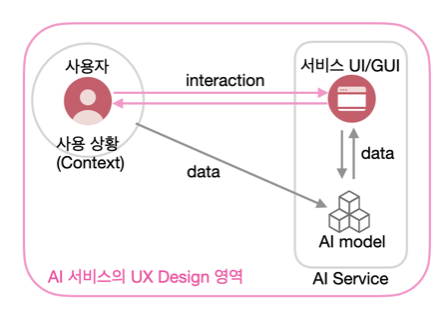
\includegraphics{img/part 1/1-2-1.png}

}

\caption{그림1: 사용자, AI Service, AI model과 UX Design의 관계
다이어그램}

\end{figure}%

\subsection{UX 디자인 대상으로서의 AI와 UX 디자인 도구로서의
AI}\label{ux-uxb514uxc790uxc778-uxb300uxc0c1uxc73cuxb85cuxc11cuxc758-aiuxc640-ux-uxb514uxc790uxc778-uxb3c4uxad6cuxb85cuxc11cuxc758-ai}

본 교재의 학습 주제는 데이터 기반 디자인이므로 UX 디자인과 AI의 두가지
연결 지점에서 사용하는 데이터의 특징을 살펴보겠습니다. 첫번째 연결
지점은 인공지능 서비스가 UX 디자인의 대상이 되는 경우, 즉 인공지능
서비스 개발을 위한 UX 디자인을 하는 지점입니다. 이 경우에 디자이너가
다루는 데이터는 인공지능 서비스가 학습하고, 테스트하고, 수집하는 사용자
및 서비스 관련 데이터가 디자인의 대상이 됩니다. 보통 디자이너는 인공지능
서비스 개발에서 사용자가 접하는 화면 그래픽(GUI)이나 인터렉션을
디자인하는 업무에 한정된다고 생각하기 쉽지만, 인공지능 서비스가 어떤
사용자 경험을 수집하고 이해해야 효과적인 서비스가 가능한지를 판단하려면
인공지능 모델 개발의 초기 단계부터 UX 디자이너가 참여해야합니다.

디자이너는 인공지능 모델을 구축할 때 인공지능이 학습할 데이터의 내용과
형식에 대하여 이해하고, 서비스의 환경과 사용자 상황에 맞는 학습 데이터를
선정하는 일에 참여합니다. 또한 인공지능 모델이 구축된 후에 성능을
테스트하고, 서비스의 완성도를 검증하는 일에도 참여해야합니다. 그리고
인공지능 서비스가 제공될 때, 사용자가 서비스와 잘 소통하고, 서비스
내용을 이해할 수 있는 사용자 접점을 디자인해야 합니다. 마지막으로
사용자의 피드백데이터를 기반으로 인공지능 모델과 서비스를 개선할 수 있는
디자인을 제시하여 서비스의 성장을 이끌게 됩니다. 이렇게 UX 디자이너는
인공지능 서비스 개발과 운영, 평가의 전반에 사용자 경험을 반영하여
서비스의 질을 확보하는 중요한 역할을 하고, 이를 위하여 서비스 전체
과정에서 사용되고, 생성되는 데이터에 대한 문해력이 필요하고, 인공지능
모델 개발자, 서비스 개발자 등 기술 전문가와의 협업 능력도 요구됩니다.
마찬가지로, 디자이너와의 효과적인 협업을 위하여 기술 전문가들도 사용자
경험과 디자인을 이해하는 역량이 요구되고 있습니다.

\begin{figure}[H]

{\centering 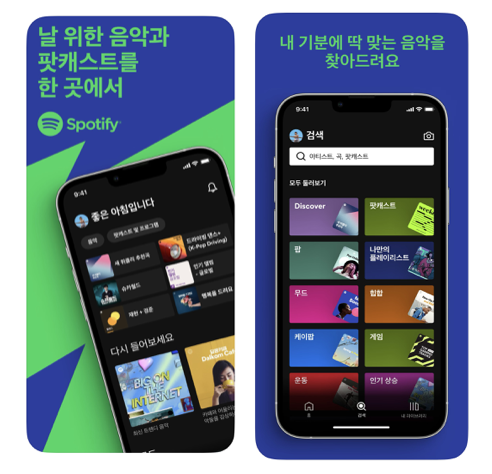
\includegraphics{img/part 1/1-2-2.png}

}

\caption{그림2: 사용자의 청취 기록을 분석하여 'Discover Weekly'와 같은
맞춤형 콘텐츠를 제공하는 글로벌 음악 스트리밍 서비스, Spotify}

\end{figure}%

두번째, 인공지능은 UX 디자인을 위한 도구 역할을 할 수 있습니다. 데이터
분석과 시각화, 아이디어 도출, 디자인 레이아웃 제안, 그래픽 시안 제작 등
디자인 프로세스의 여러 활동들이 인공지능 기술을 활용한 디자인 서비스로
제공되고 있고, 디자인하는 인공지능 서비스는 앞으로도 영역을 확장하여
발전해 나갈 것입니다. 인공지능 기술을 활용한 디자인 방법은 디자인의
생산성을 높이는 데 크게 기여하고 있습니다. 인공지능 기술은 디자이너의
사고와 작업 방식을 학습하여 디자이너처럼 데이터를 처리하고 그 결과물을
제안합니다. 이러한 상황에서 디자이너들이 기술을 더 잘 활용하고, 디자인의
역량을 확대하기 위해서는 디자인하는 인공지능 기술들이 데이터를 처리하는
방법을 이해하고 활용할 수 있어야하며, 나아가 인공지능이 더 높은 수준의
디자인 작업을 지원할 수 있도록 디자인 데이터와 디자인 행위를 데이터
기술과 연계하는 방법을 개발할 필요가 있습니다.

아래의 기사는 UX 디자인 업무에 AI 서비스를 사용하는 구체적인 업무 내용과
방법들을 설명하고 있습니다. (4)

\href{https://www.nngroup.com/articles/ai-ux-getting-started/}{AI for
UX: Getting Started}

2024년 7월에는 대표적인 UX/UI 표현 도구인 피그마에서 AI 기술을
적극적으로 활용한 디자인과 개발, 프레젠테이션 기능들을 선보였습니다. (5)

\href{https://help.figma.com/hc/ko/articles/24037640924823-Config-2024에서-발표된-새로운-기능}{Config
2024에서 발표된 새로운 기능}

이렇게 UX 디자인에 인공지능 기술이 들어와 디자이너의 업무를 수행하게
된다면 어떤 일들이 벌어질까요? 인공지능이 디자인을 할 수 있으므로
디자이너의 일자리가 없어질까요? 인공지능이 담당할 수 없는 창의적이고,
모험적인 업무에는 소수의 디자이너가 주도하고, 인공지능이 디자이너의
업무를 대신하는 것이 가능한 단순 반복적 디자인 작업이나 패턴화된 디자인
작업은 사람대신 인공지능이 대체하게 될 것입니다. 또 많은 디자이너들은
인공지능에게 할 일을 지시하거나 인공지능의 결과물을 검수하는 일, 그리고
인공지능이 디자인 업무를 할 수 있도록 디자인 업무를 디지털 데이터
중심으로 변환하고, 패턴화하는 일을 하거나, 인공지능에게 학습 데이터를
제공하는 일들을 하게 될 것입니다. 이렇게 인공지능 기반 디자인 도구들은
디자이너의 업무 내용이나 업무 역량의 변화를 이끌고, 디자인 전문가가 아닌
사람들과 디자인 업무의 협업자들이 인공지능 서비스를 활용하여 쉽게 UX
디자인 문제들을 해결하게 할 것으로 예상합니다. 기술은 본래 의식이
없습니다. 기술이 우리에게 긍정적인 역할을 할지, 부정적인 역할을 할지는
인간의 사용 의도에 따라 달라질 수 있습니다. 디자이너는 중립적인 인공지능
기술이 우리에게 유리한 방향으로 기여하도록 잘 이끌어 가야 하겠습니다.

(문헌 3) Spotify(스포티파이), Apple app store

(문헌 4) Kate Moran, Jakob Nielsen, ``\textbf{AI for UX: Getting
Started'',}
\url{https://www.nngroup.com/articles/ai-ux-getting-started/}, (2023)

(문헌 5) Figma Learn, ``\textbf{Config 2024에서 발표된 새로운 기능'',}
\url{https://help.figma.com/hc/ko/articles/24037640924823-Config-2024\%EC\%97\%90\%EC\%84\%9C-\%EB\%B0\%9C\%ED\%91\%9C\%EB\%90\%9C-\%EC\%83\%88\%EB\%A1\%9C\%EC\%9A\%B4-\%EA\%B8\%B0\%EB\%8A\%A5},
(2024)

\chapter{1-3. 데이터 기반 디자인 (Data Driven
Design)}\label{uxb370uxc774uxd130-uxae30uxbc18-uxb514uxc790uxc778-data-driven-design}

데이터 기반 디자인(Data Driven Design)이란 디자인 대상과 관련된 방대한
정량화 데이터를 디자인 설계와 의사 결정의 근거로 활용하는 기법과 정량화
테스트를 통하여 디자인 결과물을 평가, 검증하는 기법을 말합니다.(6) 쉽게
말하면, 데이터에 근거하여 디자인 의사 결정을 수행하는 기법이라고 할 수
있습니다. 데이터 기반 디자인 방법론은 디지털 데이터들을 지속적으로
생산하고 축적하는 웹이나 앱 기반 서비스에 쉽게 적용되기 때문에 구글 등
IT 서비스 기업들이 디지털 서비스의 개발과 운영에 활용하고 있습니다.
현재의 데이터 기반 디자인 연구들은 대부분 인터넷을 통하여 수집된 사용자
로그 데이터를 대상으로 이루어지고 있으나, 점차 사물인터넷(IoT: Internet
of Things) 센서 데이터를 사용하는 등 더 다양한 데이터 자원을 활용하는
방향으로 발전하고 있습니다.

데이터 기반 디자인 서비스 및 컨설팅을 제공하는 산업은 증가 추세에
있으며, 디지털 콘텐츠(웹/앱 서비스)의 사용자 로그 데이터를 시각화하여
사용자 유입 분석, 사용 행태 분석, A/B 테스팅 분석 결과를 제공하는
서비스가 주를 이룹니다. 데이터 기반 디자인을 수행하기 위하여 정량적 통계
분석 및 데이터 시각화 서비스를 지원하는 도구 및 컨설팅 비즈니스 사례에는
구글 애널리틱스(Google Analytics), 태블로(Tableau), 어도비 타깃(Adobe
Target) 서비스 등이 있으며, 각 서비스에 대하여는 다음 단원에서 자세히
다루도록 하겠습니다. (7)

앞서 인공지능 서비스를 디자인하기 위해서는 디자이너가 데이터에 대한
이해가 풍부해야한다고 설명했는데, 선행 연구에 의하면, 인공지능 서비스
개발을 위하여 디자이너는 서비스 및 사용자 관련 데이터를 원격으로 수집할
수 있는 능력과 수집된 데이터에 대한 정량적이고 정성적인 분석과 시각화를
통하여 사용자 행동을 해석하여 디자인에 반영할 수 있는 능력이 요구됩니다.
그리고 실제로 인공지능 서비스를 개발하는 디자이너들은 데이터 중심의 업무
환경에서 데이터의 기초적 통계 분석, 데이터 시각화, A/B 테스팅 기법을
매우 자주 사용하고 있다고 합니다. 그러므로 연구 팀은 디자이너가 데이터로
생각하고, 데이터로 작업하며, 데이터 전문가들과 소통할 수 있도록 하는
교육 과정을 UX 디자인 교육에 반영해야 한다고 주장하고, 또한 UX, HCI
교육에서 디자이너, 데이터 전문가, 엔지니어, 사용자 연구자 등이 함께
협업하는 학제적 수업을 제공하여 학생들이 협업 능력과 창의성을 기를 수
있도록 해야 한다고 제안하였습니다.(8) 선행 연구에서 제시한 바와 같이,
인공지능 서비스를 디자인하기 위한 데이터 문해력은 데이터 기반 디자인을
수행하기 위해 필요한 역량과 일치하고 있습니다. 데이터 기반 디자인을
공부하면서 인공지능 서비스의 디자인 역량을 함께 준비할 수 있다니, 더욱
기대되지 않나요? 그럼 다음 단원 부터는 구체적으로 데이터 기반 디자인의
방법들을 경험해 볼까요?

(문헌 6) Rochelle King, Elizabeth Churchill, and Caitlin Tan,
『Designing with data』, O'reilly, (2017), pp.3-6

(문헌 7) 이현진, 『데이터 드리븐 디자인』, UX리뷰, (2024), pp.43-44

(문헌 8) Qian Yang, Alex Scuito, John Zimmerman, Jodi Forlizzi, and
Aaron Steinfeld, ``Investigating How Experienced UX Designers
Effectively Work with Machine Learning'', DIS(Design Information
Systems)(2018), Hong Kong, pp.585--596

\part{\textbf{part 2. 디자인 리서치를 위한 탐구적 데이터 분석}}

\chapter{2-1 디자인 리서치와 탐구적 데이터 분석 (EDA:Exploratory Data
Analysis)}\label{uxb514uxc790uxc778-uxb9acuxc11cuxce58uxc640-uxd0d0uxad6cuxc801-uxb370uxc774uxd130-uxbd84uxc11d-edaexploratory-data-analysis}

\subsection{디자인
리서치란}\label{uxb514uxc790uxc778-uxb9acuxc11cuxce58uxb780}

디자인 리서치란 디자이너가 디자인 과정에서 디자인 문제를 이해하고, 주요
의사결정을 하기 위해 여러 관련 데이터를 수집, 분석, 모델링하는 과정을
말합니다. UX 디자인의 특징에 다양한 디자인 리서치 방법론이 포함될 정도로
디자인 리서치는 UX 디자인에서 매우 중요한 과정입니다. 디자인 리서치
대상인 데이터는 보통 사용자와 관련한 데이터, 프로젝트와 관련된 데이터,
그리고 프로젝트에 영향을 주는 시대나 사회, 기술의 변화에 관련한
데이터들이 포함됩니다. 디자이너는 이러한 데이터들을 적절한 방법으로
이해하고 분석하여 디자인 의사결정에 필요한 중간 산출물을 도출합니다.
디자인 리서치 과정을 통하여 디자이너가 만들어내는 중간 산출물 정보는
사용자 조사나 경쟁 제품 분석 보고서, 어피니티 다이어그램, 사용자
페르소나, 사용자 여정 지도, 콘텐츠 정보 구조도, 스토리보드, 서비스
프로토타입 등입니다. 이렇게 생성된 정보들은 디자인 해결안의 방향과
내용을 결정하는 근거가 됩니다. 그러므로 디자인 리서치가 디자인 결과물의
성공을 좌우한다고 볼 수도 있습니다. 결과적으로, 디자인 리서치는 사용자의
만족도를 높이고 비즈니스 목표를 달성하는 데 중요한 역할을 합니다.

\subsection{탐구적 데이터
분석이란}\label{uxd0d0uxad6cuxc801-uxb370uxc774uxd130-uxbd84uxc11duxc774uxb780}

탐구적 데이터 분석(EDA, Explanatory DataAnalysis)은 데이터 과학의 데이터
분석 방법 중의 하나로, 데이터 시각화 기술을 사용하여 데이터의 특징을
탐지하고 트렌드나 패턴을 확인하여 인사이트를 발견하는 데이터 분석
방법입니다. 탐구적 분석은 데이터 분석의 초기 단계에서 가장 많이
사용되고, 깊은 통찰력을 제공하며 분석 결과를 시각적으로 제시함으로써
비전문가들도 내용을 쉽게 이해할 수 있게 하는 특징이 있습니다. 데이터
분석 소프트웨어 플랫폼 기업인 Posit의 수석 과학자인 해들리 위컴(Hadley
Wichham)은 탐구적 데이터 분석 방법을 통하여 각 변수 별로 일반적인 값과
비정상적인 값의 상태, 변수 간의 상관관계와 구조를 확인할 수 있다고
하였습니다. 그는 저서에서 탐구적 데이터 분석 과정에 대하여 {[}그림
4{]}와 같이 표현했는데, 먼저 데이터를 가져오기 하여(Import) 정리한(Tidy)
뒤, 데이터를 분석에 적합한 형태로 변형하고(Transform), 데이터
시각화(Visualize)와 데이터 모델링(Model)을 반복적으로 수행하여 목표한
분석 결과가 나오면, 분석 내용을 이해하기 좋은 형태로
소통한다고(Communicate) 설명합니다.

\begin{figure}[H]

{\centering 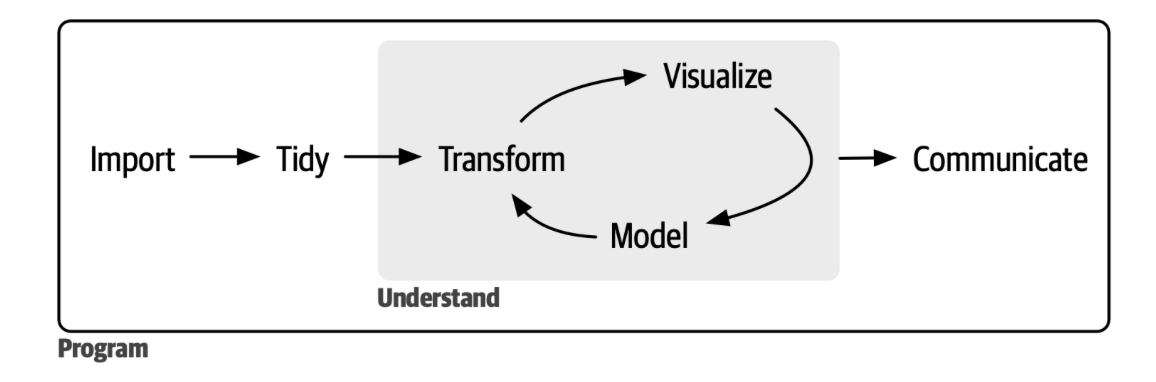
\includegraphics{img/part 2/eda.png}

}

\caption{그림 4: 탐구적 데이터 분석 프로세스 다이어그램(9)}

\end{figure}%

\subsection{디자인 리서치와 탐구적 데이터 분석의
만남}\label{uxb514uxc790uxc778-uxb9acuxc11cuxce58uxc640-uxd0d0uxad6cuxc801-uxb370uxc774uxd130-uxbd84uxc11duxc758-uxb9ccuxb0a8}

탐구적 분석에서 데이터(문제)의 현황을 탐지하고 트렌드나 패턴을 통하여
인사이트를 발견한다는 것은 더블 다이아몬드 디자인 프로세스 모델의
앞부분인 문제의 발견과 정의 단계에서 하는 활동과 매우 유사한 방법입니다.
다만 디자이너는 이 작업을 다양한 형식(비정형)의 자료를 대상으로 하고
통계 기법을 포함하여 정량, 정성, 직관적인 연구 기법을 다양하게 사용하여
수행하지만, 데이터 과학에서는 대상 데이터 형식을 정제하여 통계적 분석과
통계적 시각화 기법으로 결과를 도출한다는 점이 다릅니다.

그리고 위컴이 제시한 {[}그림 4{]}의 '탐구적 데이터 분석 프로세스
다이어그램'에는 데이터의 탐색이 의미 있는 인사이트를 발견할 때까지
반복적으로 수행되는 속성이 표현되어 있는데, 이는 디자인 프로세스의
반복적 속성과도 상통합니다. 그래서 교재의 데이터 기반 디자인
실습과제에서는 디자인 리서치 과정에서 탐구적 데이터 분석 방법을
적극적으로 활용하여 프로젝트를 진행하고자 합니다. 앞으로의 디자인 리서치
실습 과제에서 데이터 시각화 그래프들을 도출하거나, 이미 공개된 분석
보고서의 그래프들을 수집하여 그래프들의 인사이트를 도출하는 탐구적
데이터 분석 방법을 사용할 예정입니다.

(문헌 9)Hadley Wichham, Garrett. Grolemund, 『R for Data Science(2e.)』,
(2023), \url{https://r4ds.hadley.nz/intro}

\chapter{2-2 디자인 리서치를 위한 탐구적 데이터 분석 사례 (1): 서울시
미세먼지 측정 데이터 분석
사례}\label{uxb514uxc790uxc778-uxb9acuxc11cuxce58uxb97c-uxc704uxd55c-uxd0d0uxad6cuxc801-uxb370uxc774uxd130-uxbd84uxc11d-uxc0acuxb840-1-uxc11cuxc6b8uxc2dc-uxbbf8uxc138uxba3cuxc9c0-uxce21uxc815-uxb370uxc774uxd130-uxbd84uxc11d-uxc0acuxb840}

앞 장에서 탐구적 데이터 분석 방법을 통하여 각 변수 별로 일반적인 값과
비정상적인 값의 상태, 변수 간의 상관관계와 구조를 확인할 수 있다고
하였습니다. 이번에는 실제 데이터의 탐구적 분석 사례를 통하여 변수와 값의
현황과 패턴을 어떻게 도출하는지 살펴보도록 하겠습니다.

\subsection{미세먼지 정보 앱 디자인을 위한 미세먼지 데이터 분석 사례
개요}\label{uxbbf8uxc138uxba3cuxc9c0-uxc815uxbcf4-uxc571-uxb514uxc790uxc778uxc744-uxc704uxd55c-uxbbf8uxc138uxba3cuxc9c0-uxb370uxc774uxd130-uxbd84uxc11d-uxc0acuxb840-uxac1cuxc694}

다음의 데이터 분석 사례는 서울의 미세먼지 현황과 예보를 사용자들의 정보
요구에 맞게 안내해주는 앱 서비스를 디자인한다는 가정하에 공공
데이터(Pulblic data)로 공개되어 있는 서울시 미세먼지 측정 데이터를
탐구적 데이터 분석 기법을 사용하여 미세먼지 정보 앱 서비스 디자인을 위한
디자인 인사이트를 도출한 사례입니다. 이 사례는 빅데이터의 탐구적 분석
결과를 어떻게 디자인에 반영할 수 있는지를 연구하고자 제작한 가상
사례입니다.

분석 사례에 사용한 공공 데이터는 다음과 같습니다.

\begin{itemize}
\tightlist
\item
  서울 25개 측정소의 10년간 미세먼지 현황 데이터 (2008-2018년, 10년간의
  측정데이터)
\item
  2018년 서울 25개 구의 시간별 미세먼지 및 기타 오염물질 측정값
\item
  서울시 미세먼지/ 오염물질 측정소의 주소 정보
\item
  2018년 서울기상관측소의 날씨 데이터 (온도, 습도, 풍향)
\end{itemize}

여기에 서비스에 대한 사용자 니즈 관련 정보를 수집하기 위하여 목표
서비스와 비슷한 유사 앱 서비스에 대한 앱스토어의 사용자 평가 데이터
(`미세미세'와 `에어비주얼' 앱의 사용자 평가 데이터)도 분석하였습니다.

이 데이터들을 통하여 서비스의 사용자 니즈를 도출하고, 사용자의 미세먼지
정보 요구를 만족하기 위하여 미세먼지 현황과 미세먼지 예보 정보를 어떻게
제공해야 하는지를 데이터 분석을 통하여 발견하였고, 이 인사이트들을
앱디자인의 콘셉트에 반영하였습니다.

\subsection{1) 유사 앱 서비스에 대한 앱스토어의 사용자 평가 데이터로
사용자 니즈
발견하기}\label{uxc720uxc0ac-uxc571-uxc11cuxbe44uxc2a4uxc5d0-uxb300uxd55c-uxc571uxc2a4uxd1a0uxc5b4uxc758-uxc0acuxc6a9uxc790-uxd3c9uxac00-uxb370uxc774uxd130uxb85c-uxc0acuxc6a9uxc790-uxb2c8uxc988-uxbc1cuxacacuxd558uxae30}

다음의 {[}표 1{]}은 미세먼지 앱 `미세미세', '에어비주얼'의 앱 스토어
평가 데이터 내용 및 언급 건수입니다. 앱의 디자인은 자주 업데이트 되고,
여러 버전의 디자인 평가가 섞이게 되면 신뢰성이 떨어지므로 연구 시점인
2021년에 운영중인 디자인 버전에 대한 평가 데이터를 수집했습니다. (데이터
수집 기간: 2021.3.1-2021.5.31)

사용자들의 앱 평가 내용을 사용자 정보 데이터와 앱 사용 시점 데이터,
평가에서 언급한 서비스 내용으로 분류하여 앱의 사용자 경험과 관련한 주요
키워드를 도출했습니다.

{[}표 1{]} 미세먼지 앱 `미세미세', '에어비주얼'의 앱 스토어 평가 데이터
내용 및 언급 건수

\begin{longtable}[]{@{}
  >{\raggedright\arraybackslash}p{(\columnwidth - 6\tabcolsep) * \real{0.2500}}
  >{\raggedright\arraybackslash}p{(\columnwidth - 6\tabcolsep) * \real{0.2500}}
  >{\raggedright\arraybackslash}p{(\columnwidth - 6\tabcolsep) * \real{0.2500}}
  >{\raggedright\arraybackslash}p{(\columnwidth - 6\tabcolsep) * \real{0.2500}}@{}}
\toprule\noalign{}
\begin{minipage}[b]{\linewidth}\raggedright
주요 데이터 변수
\end{minipage} & \begin{minipage}[b]{\linewidth}\raggedright
\end{minipage} & \begin{minipage}[b]{\linewidth}\raggedright
미세미세 앱 평가내용 (총 188건 중 언급 건수)
\end{minipage} & \begin{minipage}[b]{\linewidth}\raggedright
에어비주얼 앱 평가내용(총 109건 중 언급건수)
\end{minipage} \\
\midrule\noalign{}
\endhead
\bottomrule\noalign{}
\endlastfoot
사용자 데이터 & 질병/가족구성 등 & 폐질환(2) & \\
\end{longtable}

천식 / 비염 등 질병(3) 해외서 귀국(1) 육아(1) 온 가족 사용(3) \textbar{}
육아(1) 타지역 친척 확인(1) \textbar{} \textbar{} 사용 상황 데이터
\textbar{} 사용 시점 등 \textbar{} 아침(3) 외출(1) 수시확인(2)
\textbar{} 해외 정보 확인(3) 운동, 야외활동(1) 아침(2) 환기(2) 외출(2)
수시확인(4) \textbar{} \textbar{} 서비스 내용 데이터 \textbar{} 서비스
불만 및 오류 \textbar{} 접속 오류(9) 위젯 불만 / 오류(11) 지도표기
오류(11) 시간표기 오류(5) 기타(7) \textbar{} 위치 표기 오류(5) 와치 연동
오류(4) 위젯 오류(3) 기타(3) \textbar{} \textbar{} \textbar{} 신뢰성
\textbar{} 신뢰함(16) 신뢰성 제기(8) \textbar{} 신뢰함(14) 신뢰성
제기(1) \textbar{} \textbar{} \textbar{} 앱의 장점 \textbar{} 편리한
디자인(22) 한눈에 보임(9) 상세 설명(6) 캐릭터 표현(8) 알림(4) \textbar{}
편리한 디자인(4) 한눈에 보임(2) 상세 설명(7) 지역 정보(6) 바람 방향
정보(2) \textbar{} \textbar{} \textbar{} 가치평가 (추천 / 감사 등)
\textbar{} 감사(29) 좋음(41) 잘 사용중(20) 추천 / 필수(14) \textbar{}
감사(10) 좋음(28) 잘 사용중(5) 추천 / 필수(4) \textbar{}

앱 평가 키워드 분석을 통하여 제공 정보의 신뢰성과 정확성, 요약 설명과
상세 설명이 포함된 정보의 설명성이 중요한 가치라는 것을 발견했고,
신뢰성, 정확성, 설명성을 높이기 위하여 어떻게 정보를 제공해야하는지를
미세먼지 측정 데이터의 탐구적 분석을 통하여 알아보고자 합니다.

\subsection{2) 서울시 미세먼지 측정 데이터에 대한 탐구적 분석 인사이트
도출}\label{uxc11cuxc6b8uxc2dc-uxbbf8uxc138uxba3cuxc9c0-uxce21uxc815-uxb370uxc774uxd130uxc5d0-uxb300uxd55c-uxd0d0uxad6cuxc801-uxbd84uxc11d-uxc778uxc0acuxc774uxd2b8-uxb3c4uxcd9c}

\begin{itemize}
\tightlist
\item
  변수와 값의 개념
\end{itemize}

변수(Variable)는 데이터를 구성하는 각각의 항목을 의미합니다. 예를 들어,
사람의 키, 몸무게, 나이 등이 변수입니다. 이 데이터를 통해 다양한 정보를
얻을 수 있습니다. 이번에는 서울시 미세먼지 측정 데이터의 변수에 대해
알아보겠습니다. 값 (Value)은 변수가 가질 수 있는 실제 데이터를
의미합니다. 예를 들어, 사람의 키라는 변수의 값은 170cm, 180cm 등이 될 수
있습니다.

{[}표 2{]}를 보면 시간, 측정소 번호, 미세먼지 값, 초미세먼지 값 등의
변수에 2018-01-01 00:00:00, 101, 29, 17 과 같이 한 사례에 측정된 값들이
1행에 할당되어 있습니다. 그리고 각 값은 시간, 숫자, 텍스트 등의 표현
형식을 가지며, 표현 형식에 따라 분석 방법이나 분석 결과가 달라지게
됩니다. 이렇게 변수 별로 동일한 형식의 값을 여러 사례 수집한 데이터를
분석함으로써 우리는 측정 시간과 측정 장소 별 미세먼지 농도의 현황과 같은
유용한 정보를 얻을 수 있습니다.

{[}표 2{]} 서울시 미세먼지 측정 데이터(위)와 날씨 데이터(아래)의 변수 및
값의 형식

\begin{longtable}[]{@{}
  >{\raggedright\arraybackslash}p{(\columnwidth - 12\tabcolsep) * \real{0.1429}}
  >{\raggedright\arraybackslash}p{(\columnwidth - 12\tabcolsep) * \real{0.1429}}
  >{\raggedright\arraybackslash}p{(\columnwidth - 12\tabcolsep) * \real{0.1429}}
  >{\raggedright\arraybackslash}p{(\columnwidth - 12\tabcolsep) * \real{0.1429}}
  >{\raggedright\arraybackslash}p{(\columnwidth - 12\tabcolsep) * \real{0.1429}}
  >{\raggedright\arraybackslash}p{(\columnwidth - 12\tabcolsep) * \real{0.1429}}
  >{\raggedright\arraybackslash}p{(\columnwidth - 12\tabcolsep) * \real{0.1429}}@{}}
\toprule\noalign{}
\begin{minipage}[b]{\linewidth}\raggedright
시간(월,일,시간)
\end{minipage} & \begin{minipage}[b]{\linewidth}\raggedright
측정소 번호
\end{minipage} & \begin{minipage}[b]{\linewidth}\raggedright
미세먼지 값(10pm)
\end{minipage} & \begin{minipage}[b]{\linewidth}\raggedright
초미세먼지 값(2.5pm)
\end{minipage} & \begin{minipage}[b]{\linewidth}\raggedright
월(달)
\end{minipage} & \begin{minipage}[b]{\linewidth}\raggedright
시간(시)
\end{minipage} & \begin{minipage}[b]{\linewidth}\raggedright
측정소 위치(구)
\end{minipage} \\
\midrule\noalign{}
\endhead
\bottomrule\noalign{}
\endlastfoot
2018-01-01 & & & & & & \\
00:00:00 & 101 & 29 & 17 & 1 & 0 & 종로구 \\
\end{longtable}

서울 25개 측정소의 2018년 미세먼지 데이터 : 209,785개의 측정값 (서울
25개 측정소의 2008\textasciitilde2018년 10년간 미세먼지 데이터 :
2,150,195개의 측정값도 같은 형식임.)

\begin{longtable}[]{@{}llllll@{}}
\toprule\noalign{}
시간(월,일,시간) & 기온 & 풍속 & 풍향 & 습도 & 풍향이름 \\
\midrule\noalign{}
\endhead
\bottomrule\noalign{}
\endlastfoot
2018-01-01 & & & & & \\
00:00:00 & -3.2 & 0.5 & 110 & 40 & 동남동 \\
\end{longtable}

서울 기상 관측소 (108번 측정소)의 2018년 날씨 데이터 : 8,740개의 측정값

\begin{itemize}
\tightlist
\item
  1년 간의 시간 변화에 따른 미세먼지량의 변화를 선 그래프로 표현한
  데이터 시각화 사례
\end{itemize}

{[}표 2{]}의 시간 변수와 미세먼지 값, 초미세먼지 값 변수에 대한 값의
변화를 그래프로 시각화하면 다음과 같습니다. 이 그래프를 보고 전체적으로
x축의 4월, 12월 주변 구간에서 측정량이 높게 나타나고, 여름에는
미세먼지량이 적게 나타나고 있어 미세먼지 측정량은 계절 차이가 있다고 할
수 있습니다. 전체적으로 미세먼지(빨강) 그래프가 위쪽에 자리하여 측정량이
많고, 측정량의 변동 폭도 큼을 볼 수 있습니다. 매우 높은 수치를 보여주는
지점들도 미세먼지 측정량(빨강)입니다. 그에 비하여 초미세먼지(파랑)는
변동이 작고 고르게 발생하고 있는 현황을 발견할 수 있습니다.

\begin{figure}[H]

{\centering 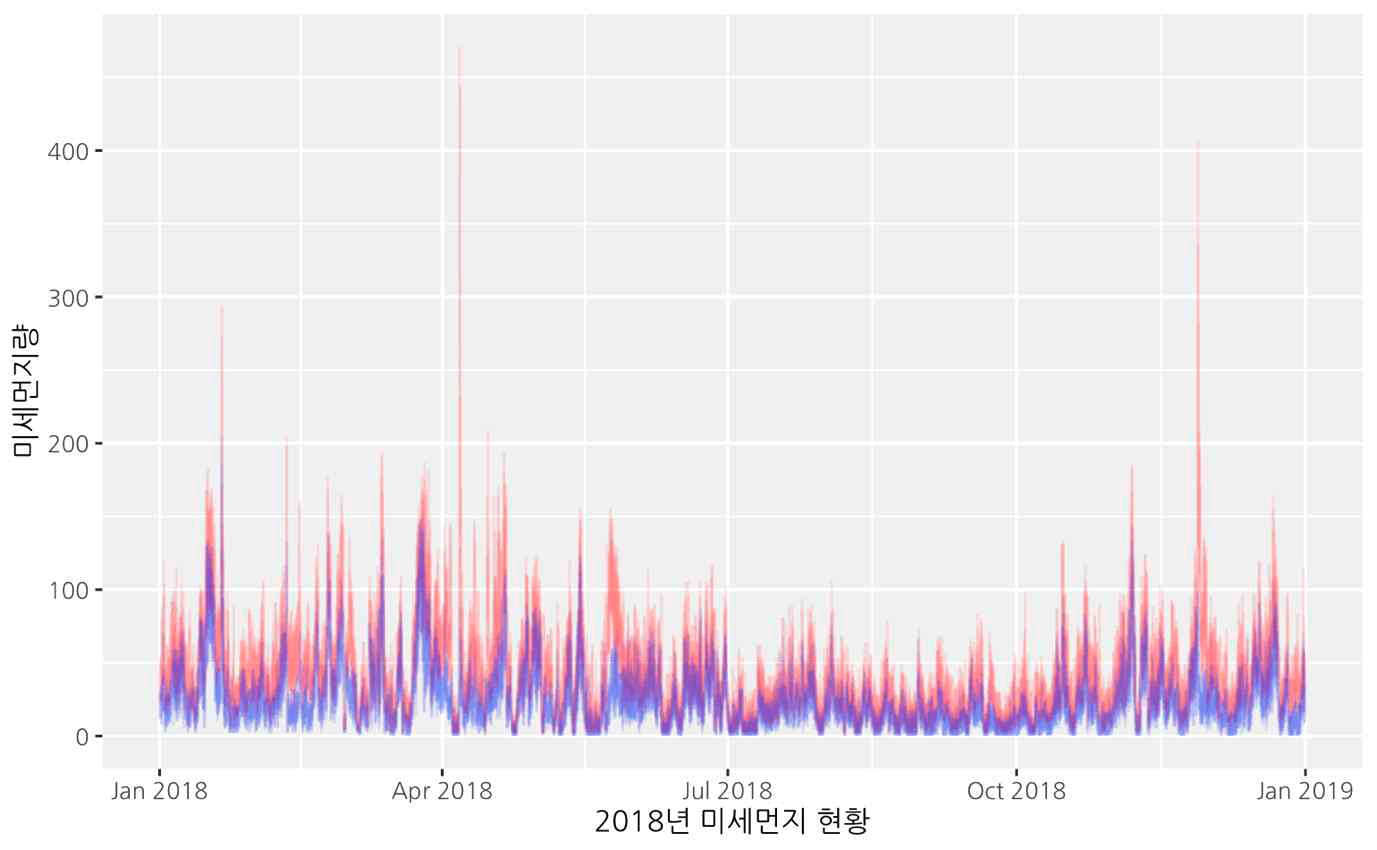
\includegraphics{img/part 2/img5.png}

}

\caption{그림 5: 2018년 서울시 미세먼지(적색)와 초미세먼지(청색)량의
측정값 현황}

\end{figure}%

\begin{itemize}
\tightlist
\item
  2018년 1-5월의 월별 일간 미세먼지 측정량 변화폭을 표현한 데이터 시각화
  그래프 사례
\end{itemize}

아래 그림은 미세먼지가 검출량이 높은 1\textasciitilde5월의 각 월별로
매일의 미세먼지 검출량의 범위가 드러나도록 한 그래프입니다. 막대 처럼
보이는 그래프 부분은 실제는 막대가 아니고 하루 동안의 미세먼지 측정량을
점으로 표현한 것이 모여서 막대처럼 보이고 있습니다. 시간 데이터 값을 월,
일로 분리하면 개별 하루의 측정 변화를 알아볼 수 있습니다. 이 그래프에서
4월 6일의 측정량 변화가 매우 큼을 확인하고, 4월 6일의 시간 별 측정
데이터를 시각화 하게 되었습니다.

\begin{figure}[H]

{\centering 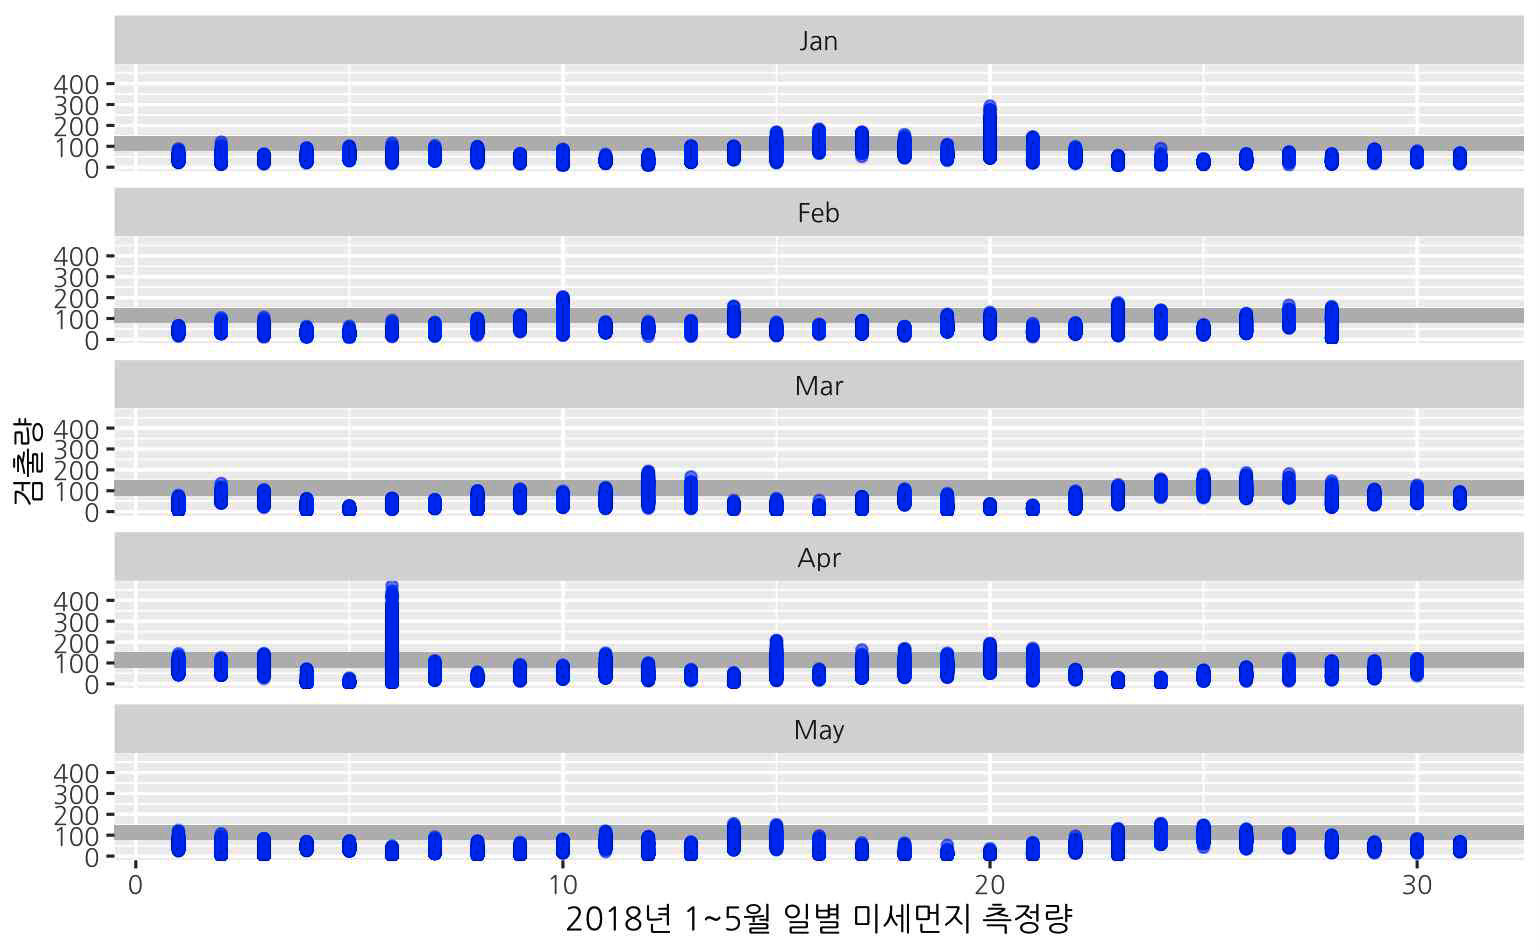
\includegraphics{img/part 2/2-3.png}

}

\caption{그림 6: 2018년 상반기(1-5월) 일별 미세먼지 측정량:미세먼지
시즌의 일별 측정량 변화를 보여준다.(회색 영역은 한국환경공단 기준
`미세먼지 나쁨' 단계 범위}

\end{figure}%

\begin{itemize}
\tightlist
\item
  2018년 4월 6일 하루 동안의 서울시 지역구별 미세먼지 측정량의 시각화
  그래프 사례
\end{itemize}

4월 6일의 미세먼지는 일간 변화량이 크고, 매우 나쁨 단계의 수치가 특정
시간대(오전 10시경\textasciitilde 오후11시경)에 집중되어 있습니다. 시간
별 측정량 차이가 크므로 미세먼지 대표값을 표현할 때 일평균 값을 쓰면
안된다는 것을 알 수 있습니다. 그리고 측정량을 꺾은선으로 표현할 때 점차
높아졌다가 낮아지는 흐름이 발견되므로 시간을 구간으로 나누어 측정량 예측
공지를 할 수 있을 것입니다.

측정소 지역별(구별) 특징을 보면 측정량을 다르지만, 시간별 측정 패턴이
다르지는 않아서 측정량의 흐름이 지역별로 동일하게 유지되고 있습니다.
매우 나쁨 단계의 측정량 범위(회색 영역 위쪽)가 너무 넓고, 같은 단계
안에서 측정량에 큰 차이가 존재합니다. 너무 넓은 변화 범위가 같은 단계로
표현되므로 매우 나쁨 단계를 더 나누어 세분화 표기할 필요가 있습니다.

\begin{figure}[H]

{\centering 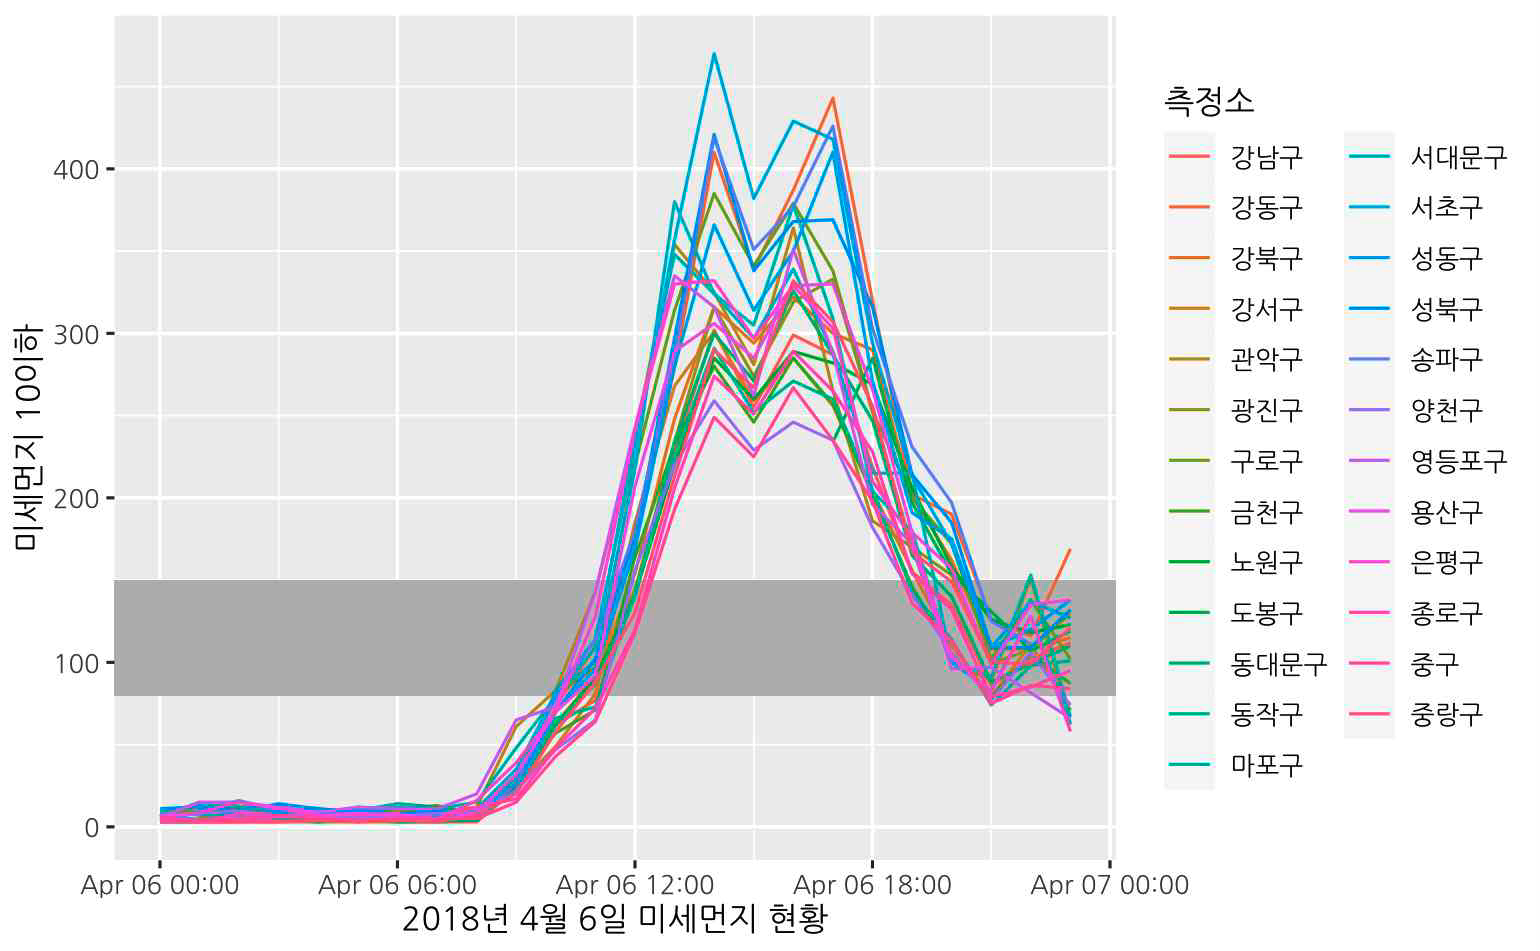
\includegraphics{img/part 2/2-2.png}

}

\caption{그림 7: 2018년 4월 6일(년간 미세먼지가 가장 심했던 날)의
시간별, 구별(지역별) 미세먼지 측정 현황(회색 영역은 한국환경공단 기준
`미세먼지 나쁨' 범위)}

\end{figure}%

\begin{itemize}
\tightlist
\item
  서울시 지역구별 미세먼지 아주 나쁨 값이 관측된 횟수 비교 시각화 사례
\end{itemize}

아래 그림은 미세먼지 아주 나쁨 단계 값이 측정된 횟수를 비교한 막대
그래프입니다. 몇 개 지역은 미세먼지 아주 나쁨 상태가 더 자주 발생하고
있음을 알 수 있고, 지역별로 횟수 차이가 존재합니다. 그러므로 특정 지역에
거주하거나 방문하는 경우에는 좀 더 적극적으로 미세먼지 상황 정보를
제공할 필요가 있어 보입니다.

\begin{figure}[H]

{\centering 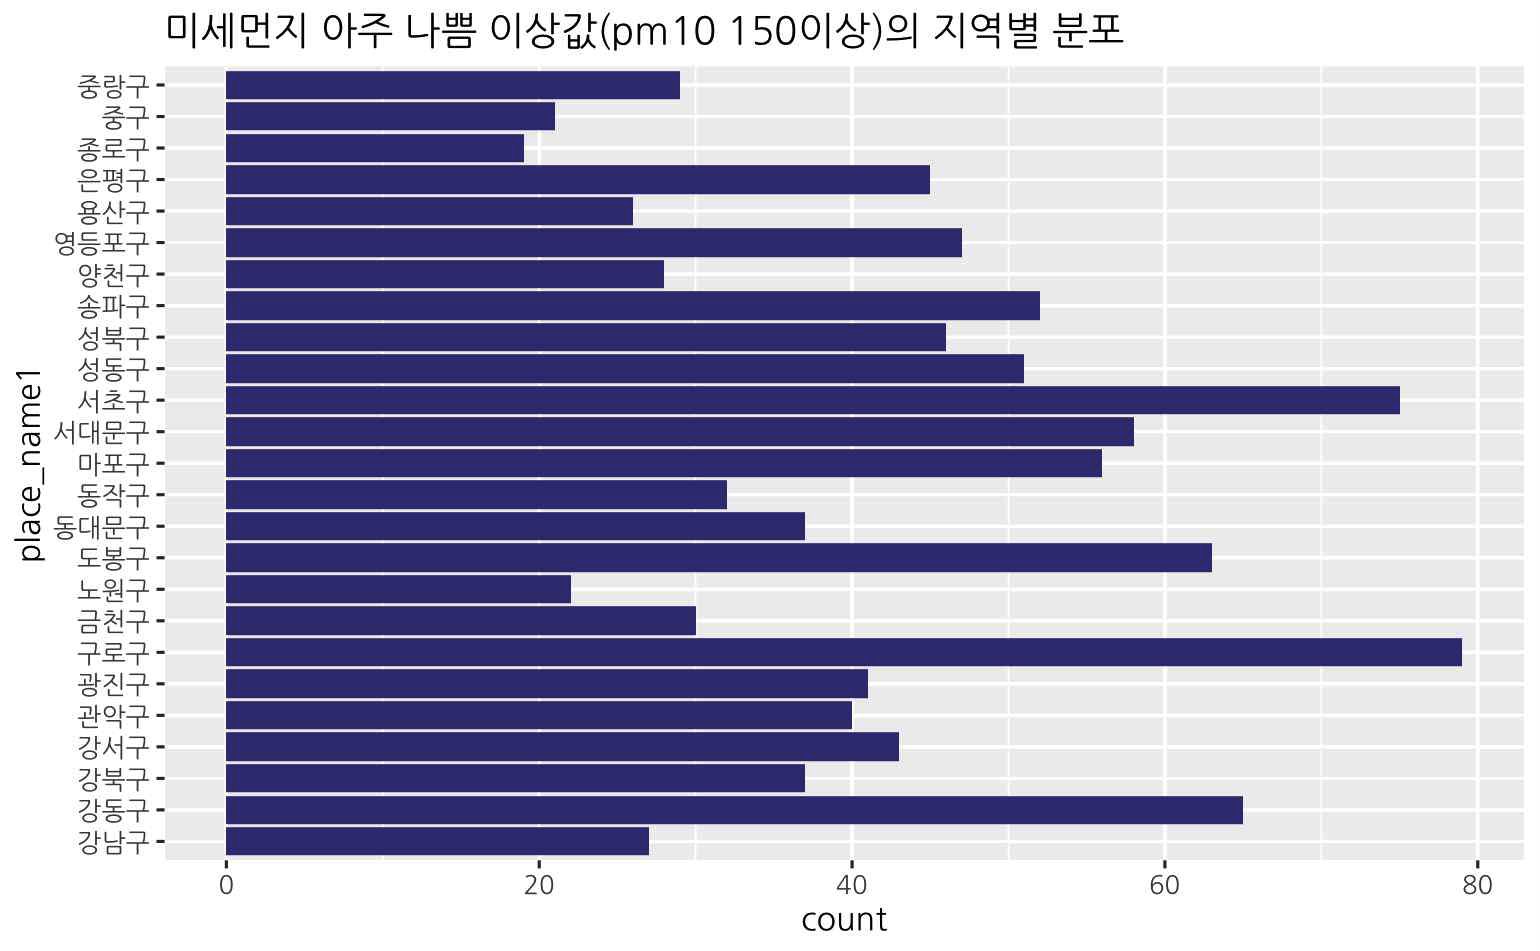
\includegraphics{img/part 2/2-5.png}

}

\caption{그림 8: 2018년 서울시 지역구별 미세먼지 `아주 나쁨' 기준 이상
값이 측정된 횟수표}

\end{figure}%

본 사례에서는 예시와 같이 다양한 변수 별, 변수 간 데이터 시각화 실험을
통하여 25건의 미세먼지와 초미세먼지 관련 변수들의 현황과 관계 패턴 및
인사이트들을 발견할 수 있었습니다. 탐구적 데이터 분석 작업의 특징은
데이터의 변수 별, 변수 간 시각화를 순차적으로 해보고, 의미 해석을 한 뒤,
그 다음에 어떤 시각화를 진행할지를 작업 과정 중에 판단하고, 앞선
분석에서 제기된 질문에 대한 답을 구하면서 단계적으로 진행하는 특징이
있습니다. 데이터 분석의 순차적이고, 가변적인 작업 과정은 디자인 리서치의
방법에서도 공통적으로 발견되는 특징입니다.

\subsection{3) 미세먼지 측정 데이터의 변수 현황 및 디자인
인사이트}\label{uxbbf8uxc138uxba3cuxc9c0-uxce21uxc815-uxb370uxc774uxd130uxc758-uxbcc0uxc218-uxd604uxd669-uxbc0f-uxb514uxc790uxc778-uxc778uxc0acuxc774uxd2b8}

{[}표 3{]}은 탐구적 데이터 분석을 통하여 발견한 서울시 미세먼지,
초미세먼지 데이터의 현황을 목록화하고, 각 결과를 바탕으로 디자인
인사이트를 도출한 사례입니다. 디자인 인사이트를 도출할 때는 1)의 사용자
니즈 발견에서 도출한 정보의 신뢰성, 정확성, 설명성 키워드를 연계하여
아이디어를 개발합니다.

{[}표 3{]} 미세먼지 및 초미세먼지 측정 데이터의 질문 사항과 분석 결과 및
데이터 패턴을 반영한 디자인 인사이트

\begin{longtable}[]{@{}
  >{\raggedright\arraybackslash}p{(\columnwidth - 4\tabcolsep) * \real{0.3333}}
  >{\raggedright\arraybackslash}p{(\columnwidth - 4\tabcolsep) * \real{0.3333}}
  >{\raggedright\arraybackslash}p{(\columnwidth - 4\tabcolsep) * \real{0.3333}}@{}}
\toprule\noalign{}
\begin{minipage}[b]{\linewidth}\raggedright
주요 변수관련 데이터의 질문 사항: 신뢰성, 데이터 제공
시점(년,월,일,시간)별 현황, 정보 설명성(요약, 상세(날씨, 지역)
\end{minipage} & \begin{minipage}[b]{\linewidth}\raggedright
분석 결과: 변수 별 값의 현황과 변수 간 상관관계
\end{minipage} & \begin{minipage}[b]{\linewidth}\raggedright
데이터 변수 패턴을 반영하는 디자인 인사이트
\end{minipage} \\
\midrule\noalign{}
\endhead
\bottomrule\noalign{}
\endlastfoot
미세먼지량과 초미세먼지량은 서로 어떤 관계가 있는가. & 대체로 양의
상관관계에 있으나 기준값 이상의 초미세먼지가 기준값 이상의 미세먼지 보다
훨씬 자주 발생한다. & 미세먼지와 초미세먼지 데이터 패턴이 다르므로
내용을 따로 표현하고, 각 패턴에 맞는 표현 방법을 사용한다. \\
년간 미세먼지와 초미세먼지 현황은 어떤 특징을 가지나? & 각 해의
상반기(4월)까지 먼지 발생이 높고, 5-10월까지는 발생량이 낮다가 11월부터
높아진다. 초미세먼지도 같은 패턴을 보이며, 일별 변동이 크다. & 월별
미세먼지 발생 시즌에 따라 다른 표현으로 안내하는 정보 서비스가 필요하다.
발생량이 낮은 기간에는 앱 사용도가 낮을 것이다. \\
월간 미세먼지와 초미세먼지 현황은 어떤 특징을 가지나? & 월 별 차이가
크다. 초미세먼지도 상반기가 많으나, 월별 먼지량의 차이가 상대적으로
작다. & \\
가을을 제외한 대부분의 달에서 기준량을 초과한다. & 초미세먼지 정보는
연중 중요도가 지속적으로 높고, 대부분 나쁨 기준량을 초과하여 경각심을 줄
필요가 있다. & \\
월간 미세면지와 시간별 미세먼지 현황은 어떤 관련성이 있나? & 미세먼지가
적은 달은 시간별 변동이 크지 않으나, 미세먼지량이 많은 달은 시간별
변동량이 크다. & 미세먼지 시즌에는 시간 별 측정량을 강조해야 한다. \\
미세먼지의 시간별 변화에 어떤 패턴이 있는가? & 미세먼지가 많은 날은 특정
시간 대에 먼지량이 집중되며, 아주 나쁨 수준에 매우 큰 편차가 존재한다.
기준 값보다 3-4배 많은 날도 있다. & 현재의 환경 공단 기준 4단계 경보는
아주 나쁨 단계의 심각성을 반영하지 못한다. 단계 구간의 변경이
필요하다. \\
초미세먼지의 시간 별 변화에 어떤 패턴이 있는가? & 초미세먼지가 많은 날은
특정 시간대에 먼지량이 집중되나 편차가 적다. & 시간별 측정량을 강조하되,
일별 정보도 의미있게 다룬다. \\
한국환경공단의 미세먼지 측정 단계는 어떤 의미가 있나? & 4단계로
되어있는데, 시간별 변동이 크므로 하루 측정값의 평균을 사용하는 표준 단계
값은 정확하지 않다. & 정확한 정보 전달을 위해 미세먼지 측정 단계 값을
일별 국내 표준이 아닌 더 \\
정확한 단계로 제공해야 한다.(기존 앱도 더 상세한 국제 기준을 사용함) &
& \\
미세먼지, 초미세먼지와 날씨는 어떤 관계가 있나? 어떤 날씨 정보가 영향을
주나? & 기온, 습도, 풍속은 크게 관련이 없고, 서, 북향의 풍향이 많은 때에
미세먼지, 초미세먼지 발생 빈도가 높다. 풍향은 계절(달)별 먼지 발생에
영향을 미친다. & 풍향 정보가 미세먼지 발생과 연계되므로, 다른 날씨
정보보다 풍향 정보를 잘 연계하여 표현해야 한다. \\
지역(측정소)별 미세먼지, 초미세먼지의 분포는 어떠한가? 지역별 차별화
표현이 필요한가? & 서울시의 구별 미세먼지 발생 패턴은 유사하다. 다만
특히 미세먼지 나쁨 단계 이상 빈도가 큰 지역이 존재한다. & 지역별로 표현
방식이 다를 필요는 없다. 그러나 발생 빈도가 높은 지역에 대한 경고 및
지역별 사용자 옵션으로 더 자세한 미세먼지 정보를 제공할 수 있다. \\
\end{longtable}

\subsection{4) 데이터 변수 패턴 기반의 디자인 컨셉
도출}\label{uxb370uxc774uxd130-uxbcc0uxc218-uxd328uxd134-uxae30uxbc18uxc758-uxb514uxc790uxc778-uxcee8uxc149-uxb3c4uxcd9c}

{[}표 4{]}는 프로젝트 데이터의 주요 변수와 키워드 별 변수 패턴을 반영한
디자인 콘셉트 제안 예시입니다. 앱 서비스에서 제공하는 정보 내용과 정보
제공 방법을 변수 패턴이 반영된 정보 표현 방법으로 제시하였습니다. 이러한
정보 표현 방법을 앱의 화면 레이아웃과 GUI에 반영하여 디자인 해결안을
완성하면, 탐구적 데이터 분석 기법을 디자인 리서치에 사용한 디자인
해결안이 됩니다.

{[}표 4{]} 프로젝트 데이터의 주요 변수와 키워드 별 변수 패턴을 반영한
디자인 콘셉트 제안 예시

주요 데이터 변수 \textbar{} 변수 관련 키워드 \textbar{} 주요 변수 패턴과
인사이트 \textbar{} 변수 패턴을 반영한

\begin{longtable}[]{@{}
  >{\raggedright\arraybackslash}p{(\columnwidth - 6\tabcolsep) * \real{0.2500}}
  >{\raggedright\arraybackslash}p{(\columnwidth - 6\tabcolsep) * \real{0.2500}}
  >{\raggedright\arraybackslash}p{(\columnwidth - 6\tabcolsep) * \real{0.2500}}
  >{\raggedright\arraybackslash}p{(\columnwidth - 6\tabcolsep) * \real{0.2500}}@{}}
\toprule\noalign{}
\begin{minipage}[b]{\linewidth}\raggedright
디자인 콘셉트
\end{minipage} & \begin{minipage}[b]{\linewidth}\raggedright
\end{minipage} & \begin{minipage}[b]{\linewidth}\raggedright
\end{minipage} & \begin{minipage}[b]{\linewidth}\raggedright
\end{minipage} \\
\midrule\noalign{}
\endhead
\bottomrule\noalign{}
\endlastfoot
사용자 데이터 & 질병/ 가족 구성 등 & & \\
사용자 특징 & 특정 사용자 집단별 서비스 니즈와 상관 없이 서비스를 자주
사용하는 사용자의 필요 반영 & & \\
서비스를 자주 사용하는(일별 사용 및 수시 사용) 일반 사용자를 타겟으로함.
& & & \\
사용 상황 데이터 & 사용 시점과 빈도, 환경(날씨, 지역) & 매일 및 수시
확인 시점 별 정보 니즈 반영 & \\
\end{longtable}

환경 정보는 지역 상황에 따라 필요성이 다름 날씨는 풍향만 미세먼지에
영향있음. \textbar{} 일별 통합 예측시 시간대별 예측 정보 제공 측정
시점(시간별) 정보, 1-3시간 후 추이 정보 강조 사용자 선택 옵션으로 지역별
날씨, 미세먼지 상세 정보 제공 \textbar{} \textbar{} 서비스 내용 데이터
(서비스 가치) \textbar{} 정보의신뢰성/ 정확성 확보 \textbar{} 년간
시즌/월별/일별/ 시간별 발생 패턴이 다름 \textbar{} 미세먼지 집중 기간
(11월-5월)과 그 외 기간의 정보 표현 차별화 여름 및 가을(6-10월)에는
미세먼지 정보 외 부가 생활 정보 제공 시간별 측정량 중심의 정보 표현
\textbar{} \textbar{} \textbar{} 정보 설명성 (요약, 상세 설명)
\textbar{} 미세/초미세 먼지의 데이터 특징이 다름 일별 요약은 대표값으로
부적절함 미세먼지의 경우 아주 나쁨 단계 범위가 너무 넓음 \textbar{}
미세, 초미세먼지의 표현 방법 차별화 미세 먼지의 아주 나쁨 단계 세분화
(초미세먼지는 그대로 사용) 아주 나쁨 단계의 경각심 표현 강화 시간별 정보
중심으로 설명 사용자 옵션으로 사용자 요구에 따른 상세 설명 방법, 알림
방법 제공 \textbar{} \textbar{} \textbar{} 관심 부가 서비스 \textbar{}
알림, 위젯 등에서 요약 정보 요구 \textbar{} 나쁨 빈도 높은 지역에는 알림
방법 강화 시간별 알림 및 관심 지역 중심의 알림, 위젯 디자인 제공
\textbar{}

이렇게 디자인 리서치에서 데이터 분석 기법을 사용하면, 적은 노력으로
다량, 장기간의 데이터를 수집 분석하는 것이 가능하여 디자인 리서치의
생산성이 높아집니다. 탐구적 데이터 분석 방법은 대규모이거나 분야간
협업이 중요한 프로젝트에서도 소통 효율을 높이는 데 기여합니다.(7)

또한 이 사례와 같이 사용자에 대한 질적 연구 방법으로는 알 수 없는 콘텐츠
데이터(미세먼지 데이터)의 특징(신뢰성, 정확성, 설명성에 영향을 미치는
정보 속성들)을 데이터 분석 기법을 통하여 발견하고, 이를 디자인 콘셉트로
개발 할 수 있습니다. 이렇게 개발한 콘셉트로 디자인을 완성한 뒤에는 과연
이 디자인이 우리가 개선하고자 한 속성들(신뢰성, 정확성, 설명성)을
개선하였는지 검증해 볼 필요가 있겠죠. 이 검증 과정이 교재의 후반부에서
학습할 A/B 테스팅 입니다.

(문헌 7) 이현진, 『데이터 드리븐 디자인』, UX리뷰, (2024), pp.100-143

\chapter{2-3 디자인 리서치를 위한 탐구적 데이터 분석 사례 (2): Stude
ntLife 데이터 분석
사례}\label{uxb514uxc790uxc778-uxb9acuxc11cuxce58uxb97c-uxc704uxd55c-uxd0d0uxad6cuxc801-uxb370uxc774uxd130-uxbd84uxc11d-uxc0acuxb840-2-stude-ntlife-uxb370uxc774uxd130-uxbd84uxc11d-uxc0acuxb840}

\subsection{StudentLife 데이터 분석 사례
개요}\label{studentlife-uxb370uxc774uxd130-uxbd84uxc11d-uxc0acuxb840-uxac1cuxc694}

\textbf{StudentLife} 연구는 2013년부터 2022년까지 다트머스 대학에서
스마트폰과 웨어러블 기기를 활용하여 학생들의 정신 건강과 행동 데이터를
분석한 장기 프로젝트입니다. 연구팀은 참여 학생들에게 스마트폰 앱을
설치하고, 스마트폰 센서를 활용하여 일상 활동, 위치, 수면 패턴, 통화
기록, 문자 메시지 등을 자동으로 수집하였고, 정기 설문 조사를
실시하였습니다. 이 데이터를 통해 학생들의 스트레스, 우울증, 불안 등의
정신 건강 상태를 평가하고, 학생 활동과 학업 성취도와의 관계를
분석했습니다. 이 연구는 장기간 수집된 데이터를 통해 학생들의 행동 변화와
정신 건강 상태를 심층적으로 연구하며, 이를 바탕으로 학생 지원 방안을
모색하였고, 스마트폰 센서 데이터를 분석하는 방법과 사례에 대한 다수의
논문을 발표하였고, 연구에서 수집한 데이터를 Kaggle 사이트에
공개하였습니다. (10)(11)

프로젝트 기간 변 주요 연구 내용은 다음과 같습니다.

\begin{itemize}
\tightlist
\item
  \textbf{2013년}: 48명의 학생을 대상으로 10주 동안 스마트폰 센서를 통해
  스트레스, 외로움, 수면 패턴 등을 분석하고, 학업 성취도(GPA)와 정신
  건강의 관계를 연구.
\item
  \textbf{2016년}: 83명의 학생을 대상으로 두 학기 동안 스마트폰과
  웨어러블 기기를 이용해 우울증과 불안의 상태를 조사.
\item
  \textbf{2018년\textasciitilde2022년}: 200명의 학생을 대상으로 COVID-19
  팬데믹 기간 포함하여 4년 동안 장기 연구를 수행하고 학생들의 정신
  건강과 행동 변화 분석.
\end{itemize}

\href{https://studentlife.cs.dartmouth.edu}{StudentLife Study}

\href{https://www.kaggle.com/datasets/subigyanepal/college-experience-dataset?resource=download}{College
Experience Study Dataset}

다음의 데이터 시각화 사례들은 본 연구에서 발표한 논문들에서 발췌한
그래프들로 여러 유형의 시각화 그래프와 그래프 해석 사례를 보여주고
있습니다. 이와같이 이미 데이터의 시각화된 분석 자료가 있는 경우, 그래프
해석을 통하여 디자인에 필요한 인사이트를 도출할 수 있습니다. 21년도에
진행한 수업에서는 아래의 그래프들을 해석하여 대학생의 행동 패턴들을
발견하고, 긍정적인 행동 패턴으로의 변화를 유도할 수 있는 모바일 서비스의
디자인 제안을 수업 프로젝트로 진행하였습니다.

다양한 유형의 데이터 시각화 그래프 해석 연습이라고 생각하고 아래에
제시한 사례 그래프들을 읽고 의미를 해석해 봅시다.

\subsection{1) 실험 참여 대학생의 학기중 생활 패턴
분석}\label{uxc2e4uxd5d8-uxcc38uxc5ec-uxb300uxd559uxc0dduxc758-uxd559uxae30uxc911-uxc0dduxd65c-uxd328uxd134-uxbd84uxc11d}

\begin{figure}[H]

{\centering 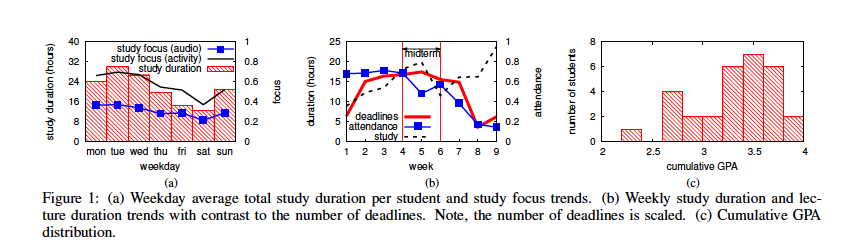
\includegraphics{img/part 2/3-1.png}

}

\caption{그림 9: 학생들의 요일(a), 학기 주차 별(b) 공부시간 패턴 변화와
학생 학점 그래프(c)(12)}

\end{figure}%

이 그래프들은 주간 요일 및 학기중 주차 별 학생들의 학업 관련 활동과
학점(GPA)을 시각화한 것입니다. 학업 활동의 변동과 학생들의 성취도를
파악함으로써, 보다 효과적인 학습 전략과 지원 프로그램을 개발하는데에
도움을 줄 수 있습니다.

\begin{itemize}
\item
  그래프 (a): 주중 평균 총 공부 시간 및 공부 집중도 추세

  X축의 요일 별로 Y축의 공부 시간 (그래프 왼쪽 축, 시간) 및 집중도
  (그래프 오른쪽 축, 0\textasciitilde1 사이의 값)을 빨간색 막대그래프:
  각 요일의 공부 시간 (study duration), 파란색 꺾은선 그래프: 오디오
  데이터를 통한 공부 집중도 (study focus (audio)), 검정색 꺽은선 그래프:
  활동 데이터를 통한 공부 집중도 (study focus (activity))로
  표현했습니다. 월요일부터 금요일에는 공부 시간과 집중도가 모두
  높습니다. 특히 주 초반에는 공부 시간이 최대치에 도달합니다. 주말에는
  공부 시간이 급격히 감소합니다. 특히 토요일에 가장 낮은 공부 시간을
  보이며, 일요일에는 약간 증가함을 알 수 있습니다.
\item
  그래프 (b): 학기 주차 별 공부 시간 및 강의 출석 시간과 과제 마감 갯수
  추세

  X축의 주차 별로(1\textasciitilde9주차까지) Y축의 공부 시간 (그래프
  왼쪽 축, 시간) 및 과제 마감 갯수 (그래프 오른쪽 축,
  0\textasciitilde1의 상대 값)를 파란색 꺾은선 그래프: 주간 출석 시간,
  빨간색 꺾은선 그래프: 주간 공부 시간, 검은색 점선 그래프: 마감 갯수로
  표현했습니다. 초기 주차 (1\textasciitilde3주차)는 공부 시간과 출석
  시간이 비교적 안정적으로 유지됩니다. 마감일 수는 적습니다. 중간고사
  기간은(4\textasciitilde6주차) 공부 시간이 급격히 증가하며, 출석 시간도
  증가합니다. 마감일 수도 증가하여 학생들이 중간고사 준비에 몰두하는
  것을 알 수 있습니다. 후기 주차 (7\textasciitilde9주차)는 공부 시간과
  출석 시간이 급격히 감소합니다. 마감일 수도 감소하여 학생들이 학기 말에
  학업 활동이 줄어드는 경향을 보입니다.
\item
  그래프 (c): 누적 GPA (모든 수강 과목의 학점 평균) 분포

  X축은 학점(GPA), Y축은 학생 수를 표현합니다. 대부분의 학생들이 3.0에서
  3.5 사이의 GPA를 가지고 있습니다. 이는 평균 이상의 학업 성취도를
  나타냅니다. 2.5 이하의 GPA를 가진 학생은 비교적 적습니다. 이는 실험에
  참여한 학생들의 전반적인 학업 성취도가 높음을 나타냅니다.
\end{itemize}

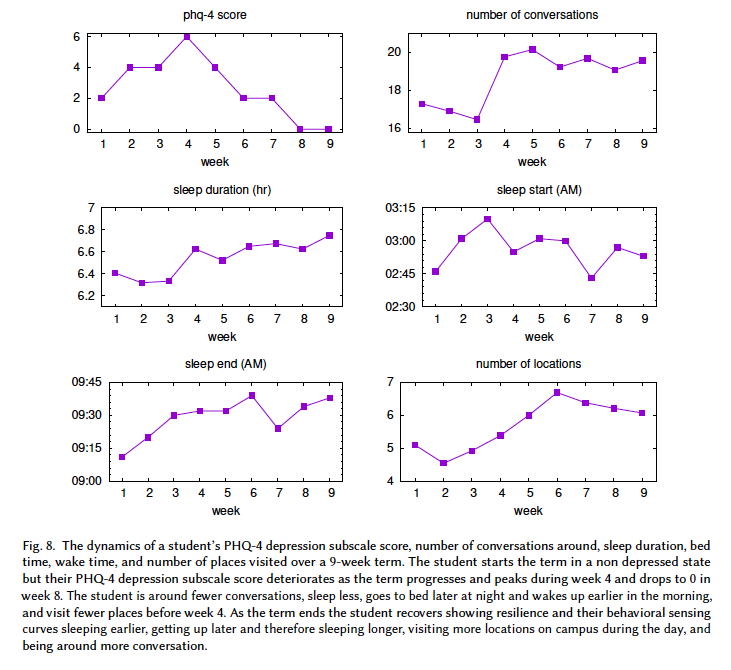
\includegraphics{img/part 2/3-2.png} 이 그래프들은 한 학생의 우울증
수준이 학기 중 특정 시기에 어떻게 변동하는지, 그리고 그에 따라 행동
패턴이 어떻게 변화하는지를 잘 보여줍니다. 이는 학생들의 정신 건강을
모니터링하고, 적절한 시기에 지원을 제공하는 데 중요한 정보를 제공할 수
있습니다. 사례 학생은 PHQ-4 점수가 초기 2주 동안 상승하여 4주차에
최고점을 기록한 후 급격히 감소하여 9주차에는 0이 됩니다. 대화 횟수는
4주에서 대화 횟수가 급격히 증가한 후 안정적으로 유지됩니다. 학기 초기
우울증 악화와 함께 사회적 상호작용이 증가합니다. 학기초 우울증 악화 기간
동안 수면 시간이 감소하다가 이후 안정됩니다. 방문 장소 수는 우울증 악화
기간 동안 적은 수의 장소를 방문하지만 회복되면서 방문 장소 수가 증가하는
패턴을 볼 수 있습니다 .

\subsection{2) 코로나 기간 동안의 학생 생활 패턴 변화
분석}\label{uxcf54uxb85cuxb098-uxae30uxac04-uxb3d9uxc548uxc758-uxd559uxc0dd-uxc0dduxd65c-uxd328uxd134-uxbcc0uxd654-uxbd84uxc11d}

\begin{figure}[H]

{\centering 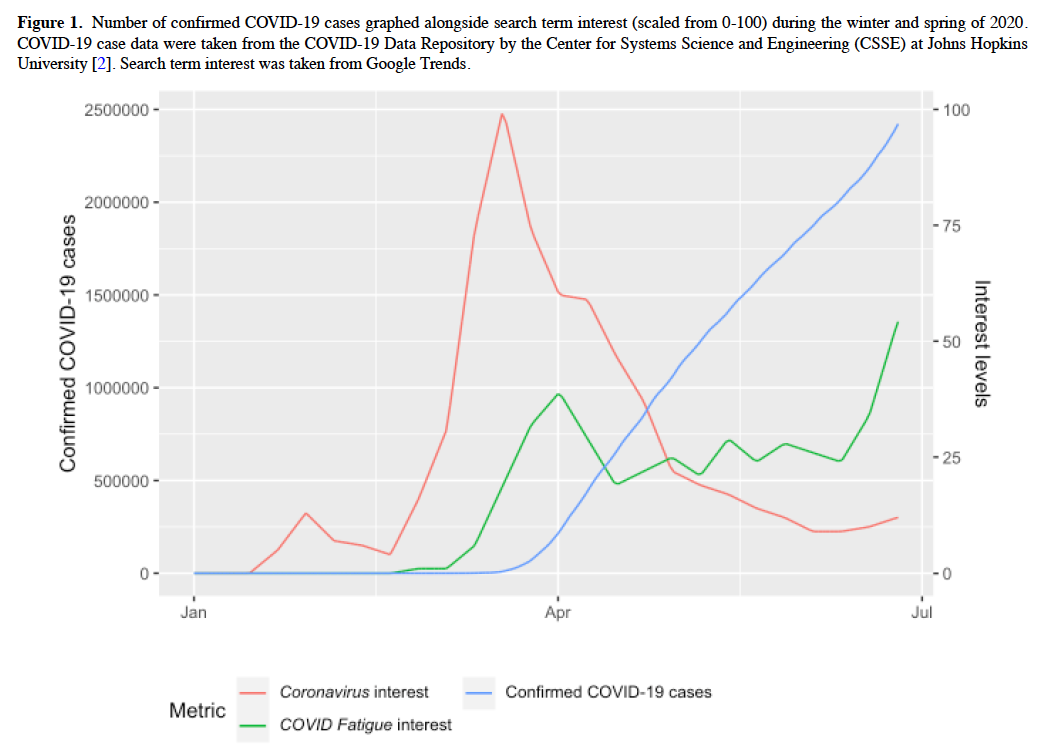
\includegraphics{img/part 2/3-3.png}

}

\caption{그림 11: 한 학생의 학기 중 PHQ-4 점수, 대화 횟수, 수면 지속
시간, 취침 시간, 기상 시간, 방문 장소 수 패턴 (14)}

\end{figure}%

위 그래프는 존스 홉킨스대에서 수집한 2020년 겨울과 봄 동안 확진된
코로나19 사례 수와 관련된 구글 검색어 관심도를 시각화한 것으로, 팬데믹
초기와 중기 동안 사람들의 정보 검색 행동과 실제 확진자 수의 변화를 잘
보여줍니다. 초기에는 바이러스에 대한 정보 검색이 활발했지만, 시간이
지나면서 코로나 증상에 대한 피로감이 증가했습니다.X축은 시간 (2020년
1월부터 7월까지), Y축의 왼쪽은 확진된 COVID-19 사례 수, Y축의 오른쪽은
관심도 수준을 (0에서 100까지, Google 트렌드 데이터) 나타내고, 파란색
선은 확진된 COVID-19 사례 수, 빨간색 선은 `Coronavirus' 검색어 관심도,
녹색 선은 `COVID Fatigue' 검색어 관심도를 나타냅니다. 확진된 COVID-19
사례 수는(파란색 선) 4월에 급격히 증가하기 시작하여 7월 초에 최고점을
기록합니다. `Coronavirus' 검색어 관심도는(빨간색 선) 3월 중순에 최고점에
도달하고, 5월\textasciitilde6월 이후 관심도가 급격히 감소하여 낮은
수준으로 유지됩니다. `COVID Fatigue' 검색어 관심도는 (녹색 선)
3월\textasciitilde4월에 관심도가 증가하여 4월 초에 첫 번째 피크에
도달합니다. 이후 관심도가 약간 감소했다가 6월 중순부터 다시 증가합니다.

4월 이후, 확진 사례 수가 계속 증가하는 반면, 'Coronavirus'에 대한
관심도는 감소하는 것은 사람들이 바이러스 자체에 대한 정보보다는 다른
주제에 더 관심을 가지기 시작했음을 시사합니다. 6월 이후 'COVID
Fatigue'에 대한 관심도가 다시 증가하는 것은 팬데믹이 장기화되면서
피로감이 더욱 심화되었음을 보여줍니다.

해당 데이터는 공중 보건 메시지 전달과 같은 커뮤니케이션 전략을 수립하는
데 중요한 인사이트를 제공하며, 팬데믹 동안 사람들의 정보 필요와 감정적
반응을 이해함으로써 더 나은 대응 전략을 마련할 수 있습니다.

\begin{figure}[H]

{\centering 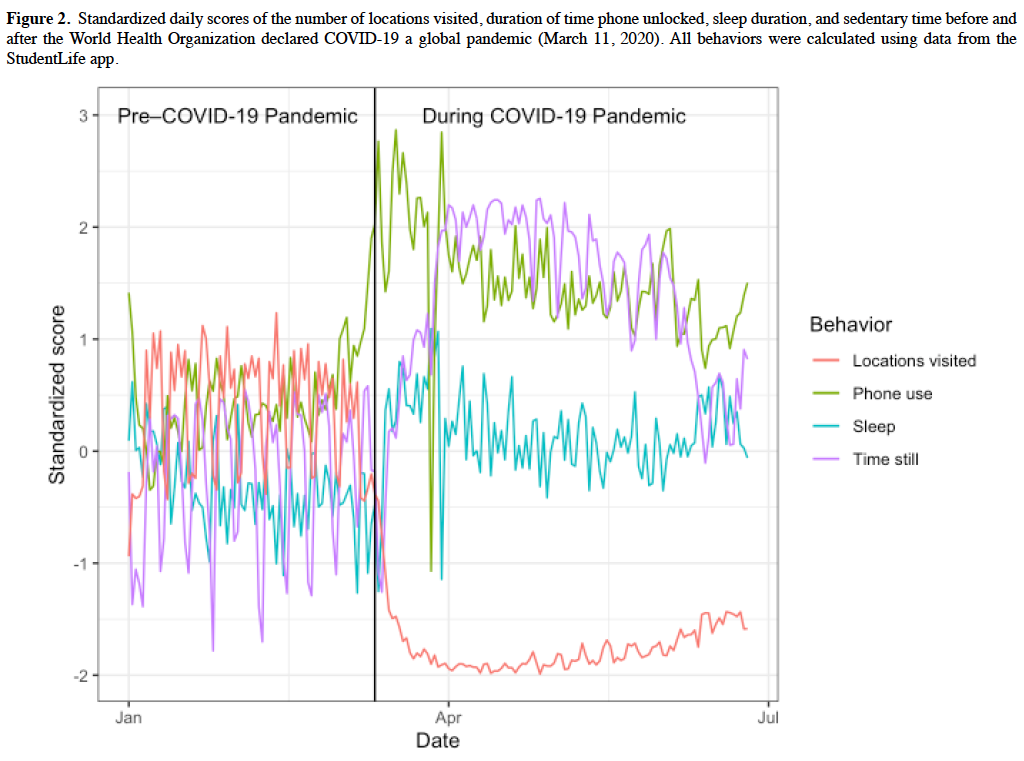
\includegraphics{img/part 2/3-4.png}

}

\caption{그림 12: 2020년 코로나 팬데믹 기간의 StudentLife 앱에 기록된
학생 활동 변화 (14)}

\end{figure}%

위 그래프는 COVID-19 팬데믹 이전과 이후의 학생들의 일상 행동 변화를
시각화한 것입니다. 여기에는 방문한 장소 수, 핸드폰 사용 시간, 수면 시간,
움직임이 없던 시간이 표준화 지표로 표현되어 있습니다. 팬데믹 선언 후
방문한 장소 수가 급격히 감소하고, 핸드폰 사용 시간과 정지 상태의 시간이
급격히 증가합니다. 또한 수면 시간도 팬데믹 이전보다 증가하는 경향을
보입니다. WHO가 COVID-19 팬데믹을 선언한 날짜 (2020년 3월 11일)전에는
모든 행동 지표가 변동성이 큽니다. 팬데믹 선언 직후 모든 행동 지표에
급격한 변화가 관찰됩니다. 팬데믹 동안(Dur방문한 장소 수는 낮은 수준을
유지하지만, 점차 증가하는 경향이 있습니다. 핸드폰 사용 시간은 팬데믹
선언 직후 급격히 증가합니다. 이는 학생들이 집에 머무르면서 온라인 활동과
소셜 미디어 사용이 증가했음을 시사합니다. 수면 시간과~정지 상태 시간은
변동이 있지만 팬데믹 이전보다 높은 수준을 유지합니다.

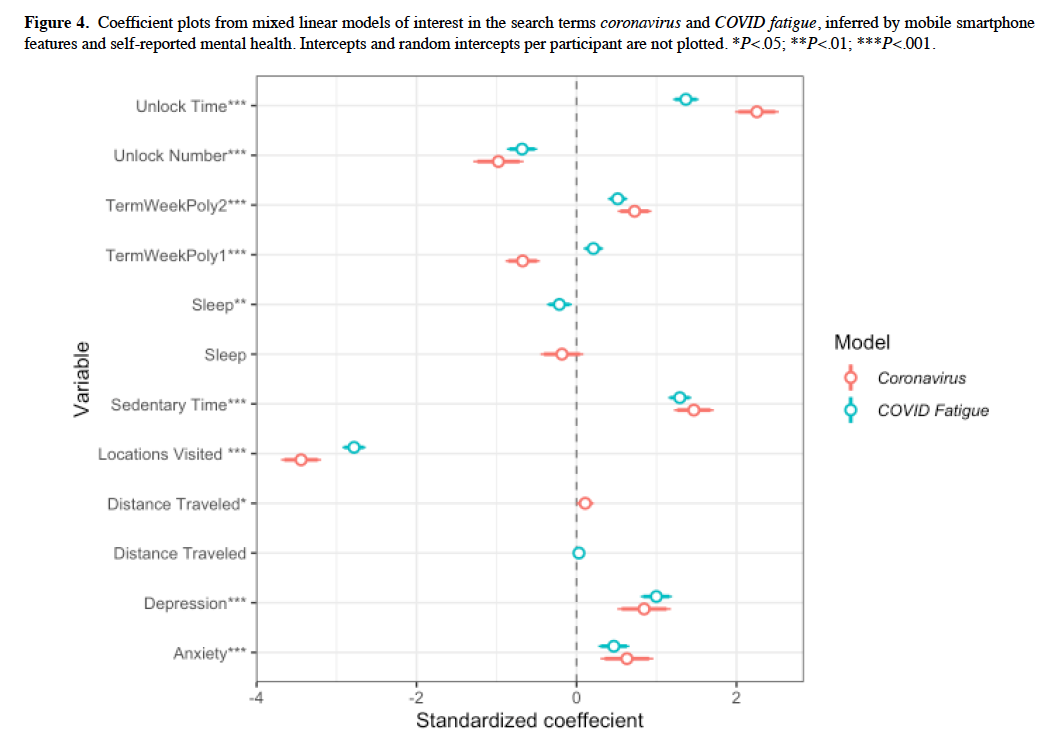
\includegraphics{img/part 2/3-5.png} 위 그래프(Coefficient plot)은
코로나 바이러스, 코로나 피로의 관심도와 학생 활동의 영향에 대한 회귀
분석 결과를 시각화한 그래프입니다. X축의 계수 값(Coefficient Value)이
클수록 해당 변수의 영향력이 크고, 계수 값이 양수면 해당 변수가 종속
변수에 정(+)의 영향을, 음수면 부(-)의 영향을 미칩니다. 이 플롯을 통해
어떤 변수가 중요한지, 그리고 그 영향력이 어떻게 되는지를 직관적으로
파악할 수 있습니다.

위 그래프에서 코로나 바이러스, 코로나 피로의 관심도는 스마트폰 사용
시간, 정적 활동의 증가와 관련이 있으며, 이동 거리와 방문 장소 수의
감소와 관련이 있습니다. 또한 우울과 걱정도 코로나 관심도가 양의 영향을
미칩니다.

\subsection{3) 코로나 기간 전후의 학생 생활 및 정신 건강 상태에 대한
데이터
분석}\label{uxcf54uxb85cuxb098-uxae30uxac04-uxc804uxd6c4uxc758-uxd559uxc0dd-uxc0dduxd65c-uxbc0f-uxc815uxc2e0-uxac74uxac15-uxc0c1uxd0dcuxc5d0-uxb300uxd55c-uxb370uxc774uxd130-uxbd84uxc11d}

이 연구는 대학생들의 정신 건강 변화를 코로나 기간을 포함하여 추적한
연구로서, 연구진은 모바일 센싱 소프트웨어를 사용하여 4년 동안 200명
이상의 대학생들의 실시간 활동 데이터를 수집했습니다.

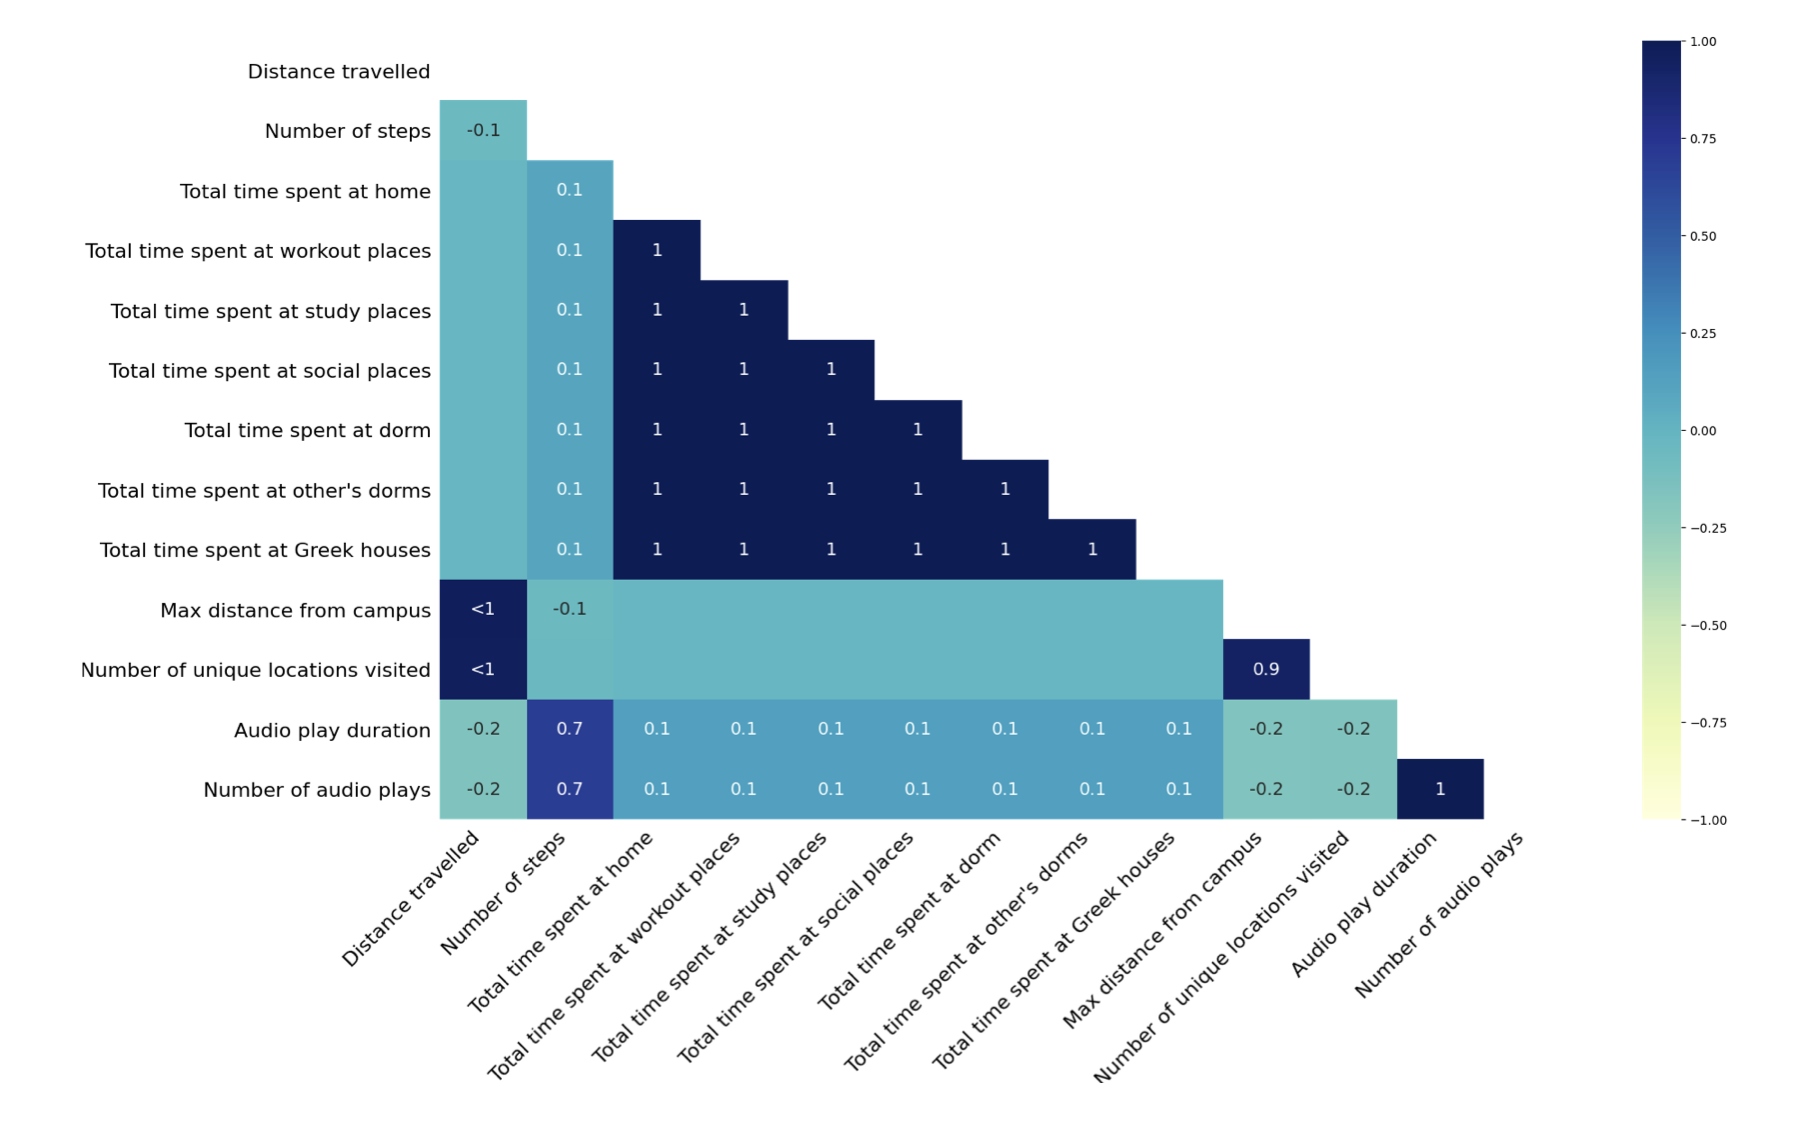
\includegraphics{img/part 2/3-6.png} Nullity Correlation은 데이터
분석에서 결측값(Missing Values) 간의 상관관계를 나타내는 용어입니다.
특정 변수의 결측값 존재 여부와 다른 변수의 결측값 존재 여부 사이의
관계를 측정합니다. 예를 들어, 두 변수 모두 결측값이 있는 경우, 이
변수들은 높은 Nullity Correlation 값을 가질 것입니다. 이는 한 변수의
데이터가 결측되면 다른 변수도 결측될 가능성이 높다는 것을 의미합니다.

{[}그림 14{]}에서, 대부분의 위치 관련 특성들은 1의 값을 가지는데, 이는
하나의 위치 특성이 나타나면 다른 위치 특성도 거의 항상 나타난다는 것을
의미합니다. 위치 특성은 GPS 데이터의 가용성에 따라 달라지기 때문에, GPS
데이터가 있을 때는 위치 특성들이 모두 존재하거나, 없을 때는 모두
존재하지 않는 것이 논리적입니다. 1.0 상관관계에 대한 예시로 ****``Total
time spent at social places''와 ``Total time spent at other's dorms''
(사회적 장소에서 보낸 시간과 다른 기숙사에서 보낸 시간)을 보면 두 장소의
데이터는 동시에 측정되었습니다. 그리고 ``Number of audio plays''와
``Audio play duration'' (오디오 재생 횟수와 오디오 재생 시간)의 0.7
상관관계는 두 기능이 자주 함께 나타남을 의미합니다. 오디오를 재생할수록
재생 시간도 증가하기 때문에 논리적인 결과입니다. 반면에 ``Audio play
duration''과 ``Total time spent at study places'' (오디오 재생 시간과
공부 장소에서 보낸 시간)간의 음의 상관관계는 상관관계가 없다고 볼 수
있습니다. 예를 들어, 운동이나 공부를 할 때 오디오를 재생하는 시간이
감소할 수 있습니다.

\begin{figure}[H]

{\centering 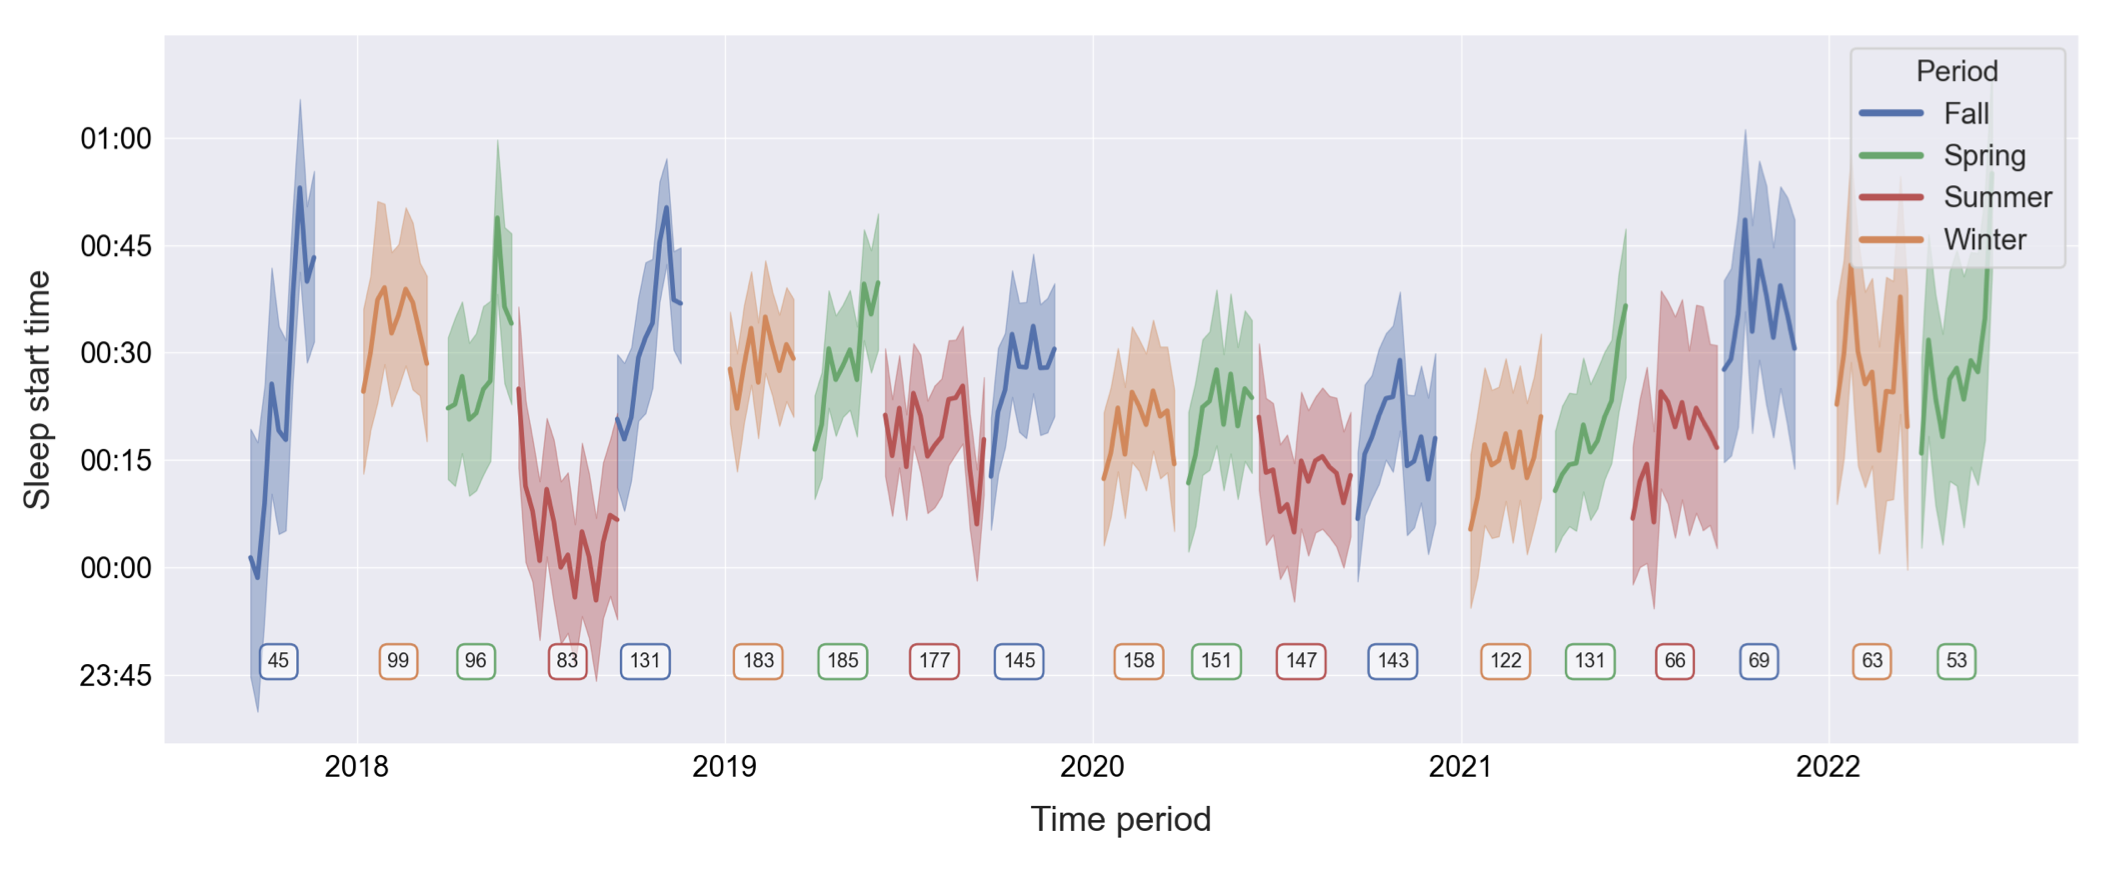
\includegraphics{img/part 2/3-7.png}

}

\caption{그림 15: 실험의 센싱 데이터 결측값(Missing Values) 간의
상관관계 그래프 (15)}

\end{figure}%

해당 그래프는 2018년부터 2022년까지 학기와 연도에 따른 학생들의 수면
시작 시간의 변화를 보여줍니다. 여름 학기 동안 학생들이 더 일찍 잠드는
경향이 있으며, 학기 말로 갈수록 수면 시간이 늦어지는 패턴이 관찰됩니다.
그리고 가을 학기(파랑)와 겨울 학기(주황)는 비교적 수면 시작 시간이
일정하게 유지되지만, 봄 학기(초록)와 여름 학기(빨강)는 더 큰 변동성을
보입니다. 각 학기의 참여자 수는 그래프 하단의 사각형에 표시되어
있습니다. 예를 들어, 2018년 가을 학기에는 45명이 데이터를 제공한 반면,
2021년 봄 학기에는 122명이 데이터를 제공하였습니다. 학기마다 다른
참여자수는 데이터의 신뢰성에 영향을 미칠 수 있습니다.이러한 정보를
통하여 학생들의 수면 습관을 이해하고, 건강한 수면 습관을 촉진하기 위한
캠퍼스 정책을 개발할 수 있습니다.

\begin{figure}[H]

{\centering 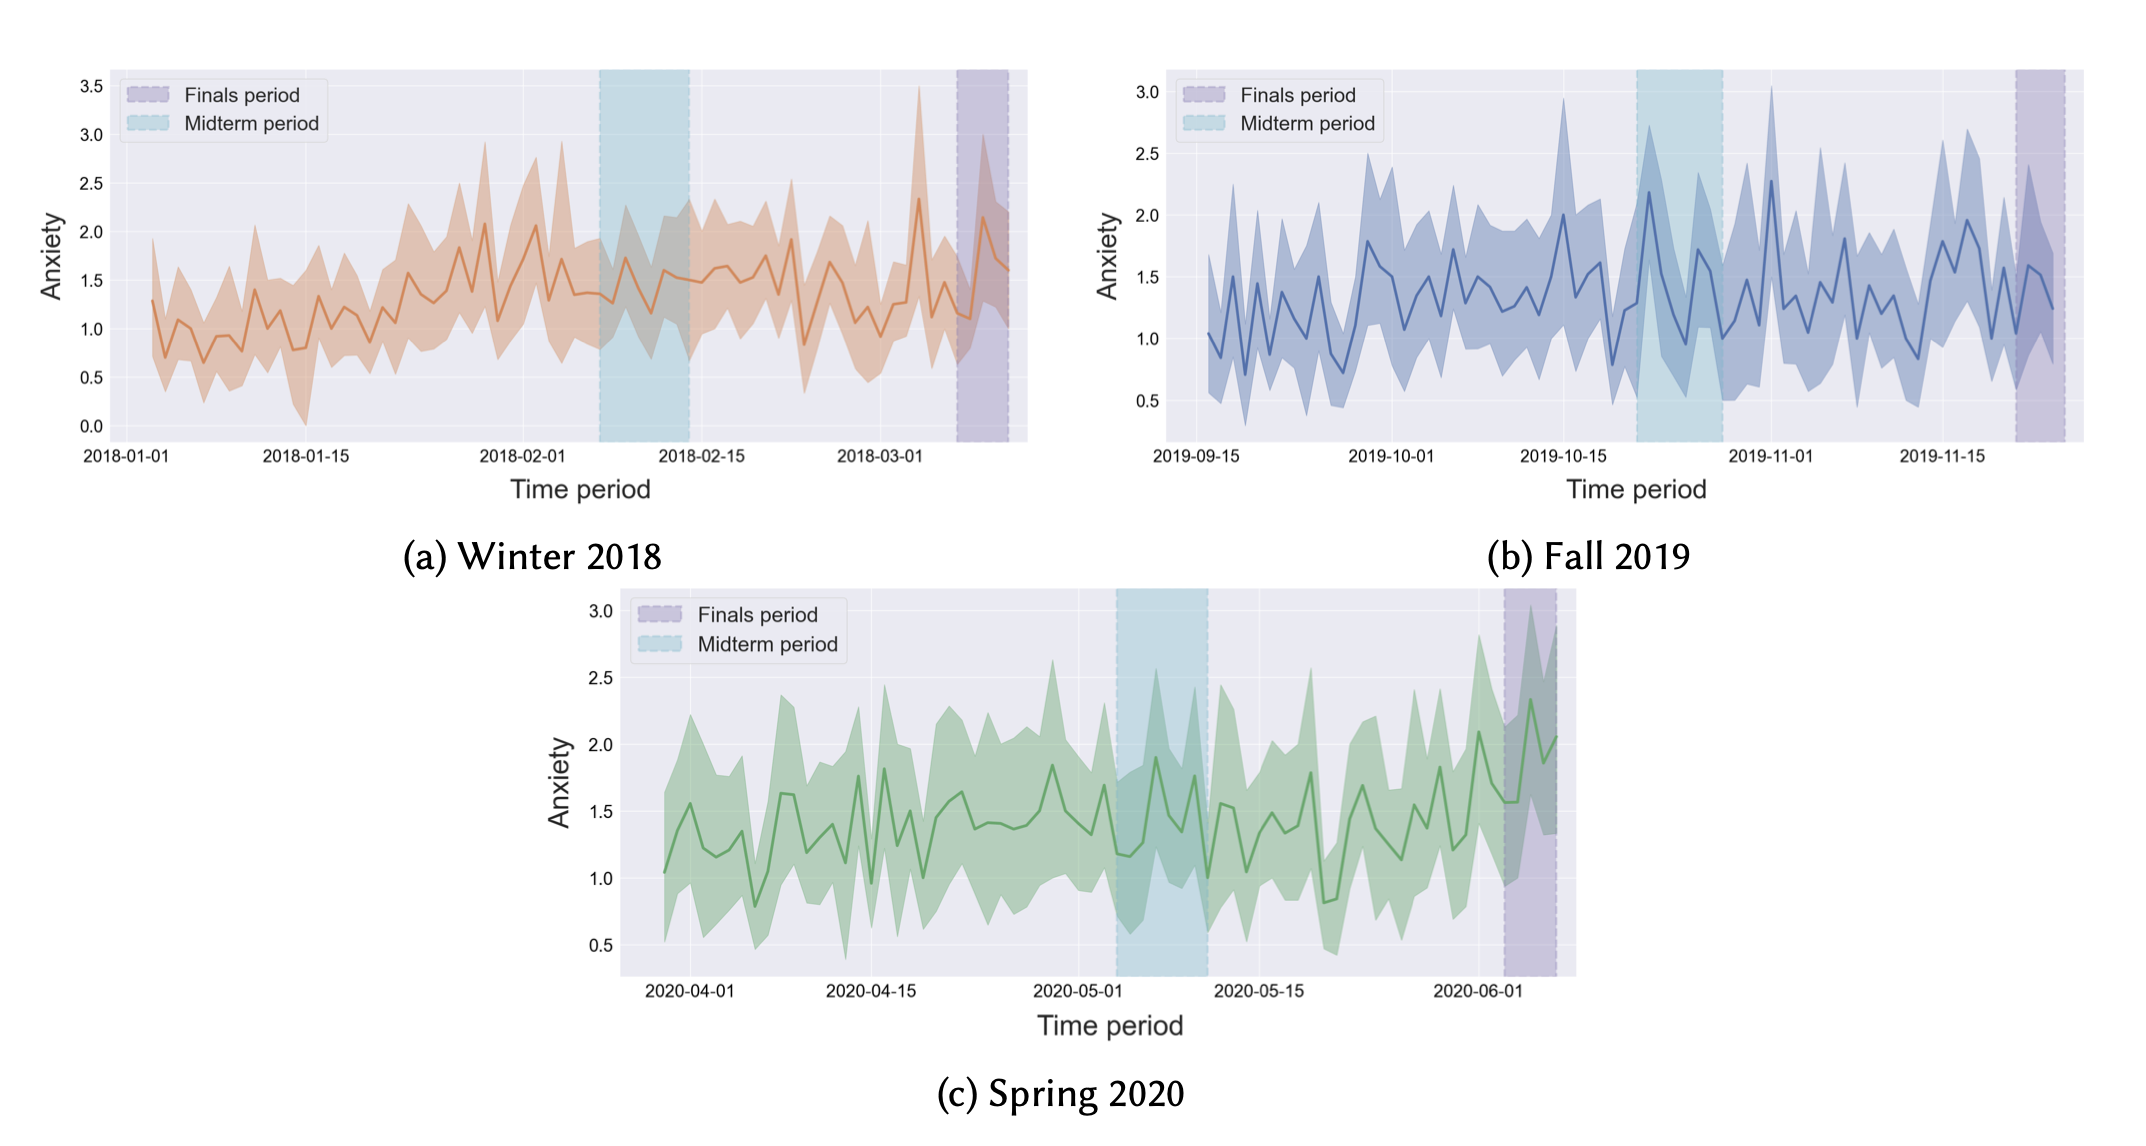
\includegraphics{img/part 2/3-8.png}

}

\caption{그림 16: 학기별 학생들의 불안 지수 변화 (15)}

\end{figure}%

이 그래프는 학생들이 중요한 학업 기간 동안 불안을 더 많이 느낀다는 것을
시각적으로 보여줍니다. 특히 중간고사와 기말고사 기간 동안 불안 점수가
상승하는 경향이 명확하게 나타납니다. 2018년 겨울 학기와 2020년 봄 학기는
불안 점수의 변동 폭이 크지만, 2019년 가을 학기는 비교적 안정적인 차이가
있어 학기별로 불안 지수가 다른 특징이 있습니다. 이러한 정보는 학생들의
학업 스트레스를 줄이고, 정신 건강을 지원하기 위한 정책을 개발하는 데
중요한 데이터로 활용될 수 있습니다.

\begin{figure}[H]

{\centering 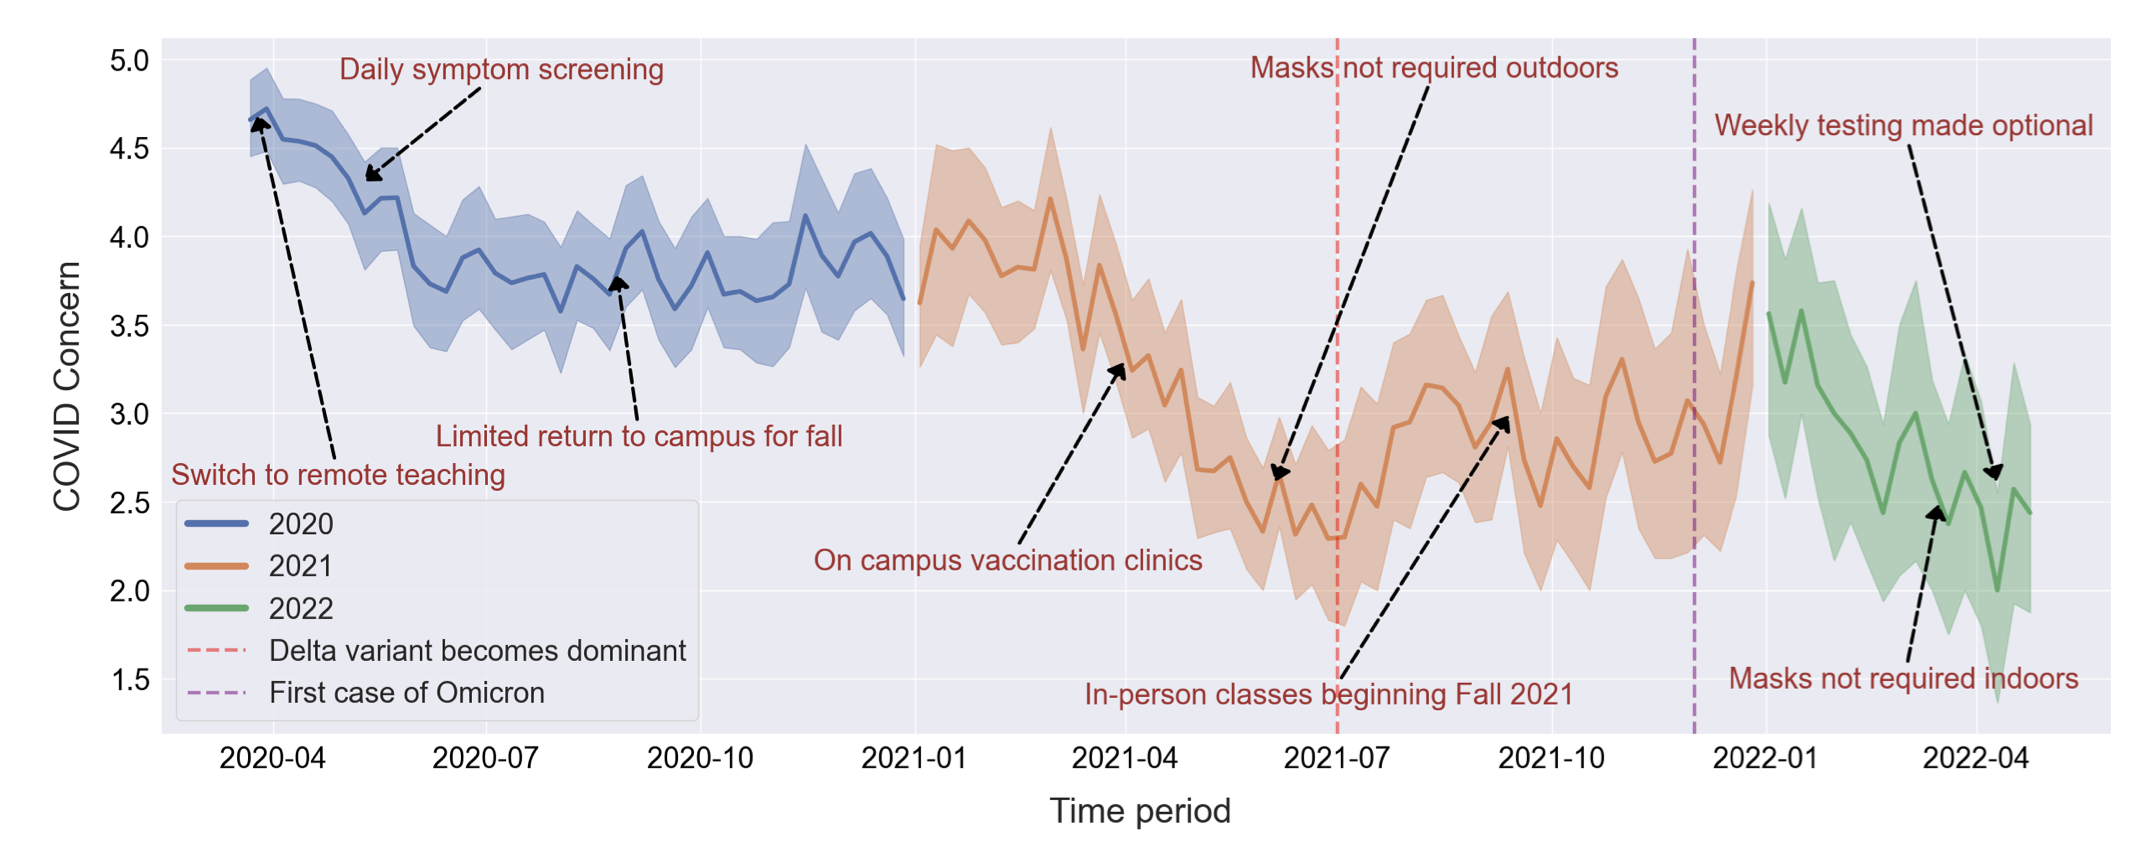
\includegraphics{img/part 2/3-9.png}

}

\caption{그림 17: 시간의 흐름에 따른 코로나 걱정 지수 변화 (15)}

\end{figure}%

이 그래프는 코로나 팬데믹 기간 동안 주요 코로나 이벤트에 따른 COVID-19에
대한 학생들의 걱정 정도를 보여줍니다. 중요한 캠퍼스 이벤트 및 조치들이
학생들의 걱정 수준에 큰 영향을 미쳤음을 알 수 있습니다. 이러한 데이터는
팬데믹 대응 및 학생 지원 전략을 수립하는 데 인사이트를 제공할 수
있습니다.

주요 이벤트와 걱정 지수의 변화:

\begin{itemize}
\tightlist
\item
  \textbf{원격 수업 전환 (2020년 4월)}: 걱정 수준이 상당히 낮아지는
  효과가 있습니다.
\item
  \textbf{일일 증상 검사 도입 (2020년 5월)}: 초기 팬데믹 대응 조치로,
  걱정 수준이 높지만 점차 감소합니다.
\item
  \textbf{캠퍼스 복귀 제한적 허용 (2020년 10월)}: 걱정 수준이 다시 약간
  상승합니다.
\item
  \textbf{백신 클리닉 도입 (2021년 4월)}: 걱정 수준이 크게 감소하는 주요
  요인입니다.
\item
  \textbf{마스크 착용 완화 (2021년 6월, 2022년 4월)}: 걱정 수준이
  감소하는 경향을 보입니다.
\item
  \textbf{델타 변이 및 오미크론 변이 출현 (2021년 7월, 2022년 1월)}:
  새로운 변이의 출현으로 걱정 수준이 다시 증가합니다.
\end{itemize}

이상의 데이터 분석 사례와 같이 여러분의 실습 주제와 관련한 데이터 분석
보고서나 논문을 찾아보고, 제시된 데이터의 분석 표나 그래프를 해석하여
디자인 주제에 대한 인사이트를 발견해보세요.

(문헌 10) Dartmouth College, ``StudentLife Study'', (2024.7.24),
\href{https://studentlife.cs.dartmouth.edu/}{https://studentlife.cs.dartmouth.edu}

(문헌 11) Kaggle, ``College Experience Study Dataset'', (2024.7.31)
\url{https://www.kaggle.com/datasets/subigyanepal/college-experience-dataset?resource=download}

(문헌 12) Rui Wang, et al., ''SmartGPA: How Smartphones Can Assess and
PredictAcademic Performance of College Students'', UbiComp '15,
September 07-11, 2015, Osaka, Japan

(문헌 13) R. Wang et. al., ``Tracking Depression Dynamics in College
Students Using MobilePhone and Wearable Sensing'', Proceedings of the
ACM on Interactive, Mobile, Wearable and Ubiquitous Technologies, Vol.
2, No.~1, Article 43. (2018).

(문헌 14) D. L Mack, et al., ``Mental Health and Behavior of College
Students During theCOVID-19 Pandemic: Longitudinal Mobile Smartphone
andEcological Momentary Assessment Study, Part II'', JOURNAL OF MEDICAL
INTERNET RESEARCH, vol.~23, iss. 6, e28892 (2021)

(문헌 15) Subigya Nepal, et al.~``Capturing the College Experience: A
Four-Year Mobile Sensing Study of Mental Health, Resilience and Behavior
of College Students during the Pandemic.'' Proceedings of the ACM on
Interactive, Mobile, Wearable and Ubiquitous Technologies. (2024)

\chapter{2-4 EDA를 위한 데이터 분석
도구들}\label{edauxb97c-uxc704uxd55c-uxb370uxc774uxd130-uxbd84uxc11d-uxb3c4uxad6cuxb4e4}

\subsection{Google Analytics (GA)}\label{google-analytics-ga}

Google Analytics는 웹사이트와 앱의 사용자 행동을 추적하고 분석하여,
마케팅 전략을 개선하고 사용자 경험을 최적화하는 데 도움을 주는
도구입니다. 이를 통해 사용자들이 어떤 경로로 사이트에 도착했는지, 어떤
페이지에서 얼마나 머무르는지, 어떤 행동을 하는지 등을 상세히 분석할 수
있습니다. 서비스에 가입하면 데이터 분석이 필요한 웹 서비스에 GA와
연계하는 코드를 삽입하여 데이터를 추출하고, 다양한 GUI 메뉴로 데이터
현황을 탐색할 수 있습니다. (16)

\href{https://marketingplatform.google.com/intl/ko/about/analytics/features/}{애널리틱스
기술 및 통합 - 애널리틱스}

\subsection{주요 서비스}\label{uxc8fcuxc694-uxc11cuxbe44uxc2a4}

\begin{itemize}
\item
  데이터 수집 및 관리

  웹사이트와 앱의 데이터를 통합하여 분석할 수 있고, 다양한 플랫폼과
  기기에서 발생하는 데이터를 정확하게 추적합니다.
\item
  분석 및 통계

  \begin{itemize}
  \tightlist
  \item
    \textbf{사용자 세그먼트}: 특정 기준에 따라 사용자 그룹을 세분화하고
    각 그룹의 행동을 분석할 수 있습니다.
  \item
    \textbf{행동 분석}: 사용자의 페이지 방문, 클릭, 이벤트 등 다양한
    행동 데이터를 분석합니다.
  \item
    \textbf{실시간 데이터}: 실시간으로 웹사이트 방문자 수, 현재 활동
    중인 페이지 등을 모니터링할 수 있습니다.
  \end{itemize}
\item
  보고 및 시각화

  \textbf{맞춤형 대시보드로} 중요한 데이터를 한눈에 볼 수 있습니다.
  데이터를 그래프와 차트로 시각화하여 쉽게 이해하고 분석할 수 있고, PDF,
  Excel 등 다양한 형식으로 보고서를 내보낼 수 있습니다.
\item
  통합 및 확장

  \begin{itemize}
  \tightlist
  \item
    \textbf{Google Ads,} Google Tag Manager, Firebase 등 다른 Google
    도구와 원활하게 연동됩니다.
  \item
    \textbf{API 지원}: 다양한 API를 통해 데이터를 추출하고 맞춤형
    솔루션을 구축할 수 있습니다.
  \end{itemize}
\item
  머신러닝 및 인사이트

  머신러닝을 활용하여 자동으로 목표를 설정하고 중요한 인사이트를
  제공합니다. 사용자의 미래 행동을 예측하고 이에 맞춘 전략을 수립할 수
  있습니다.
\item
  단점: 고급 기능을 활용하려면 일정 수준 이상의 기술 지식이 필요할 수
  있습니다. 그리고 대규모 트래픽이 발생하는 웹사이트에서는 샘플링
  데이터를 제공하여 전체 데이터를 반영하지 않을 수 있습니다.
\end{itemize}

\begin{figure}[H]

{\centering 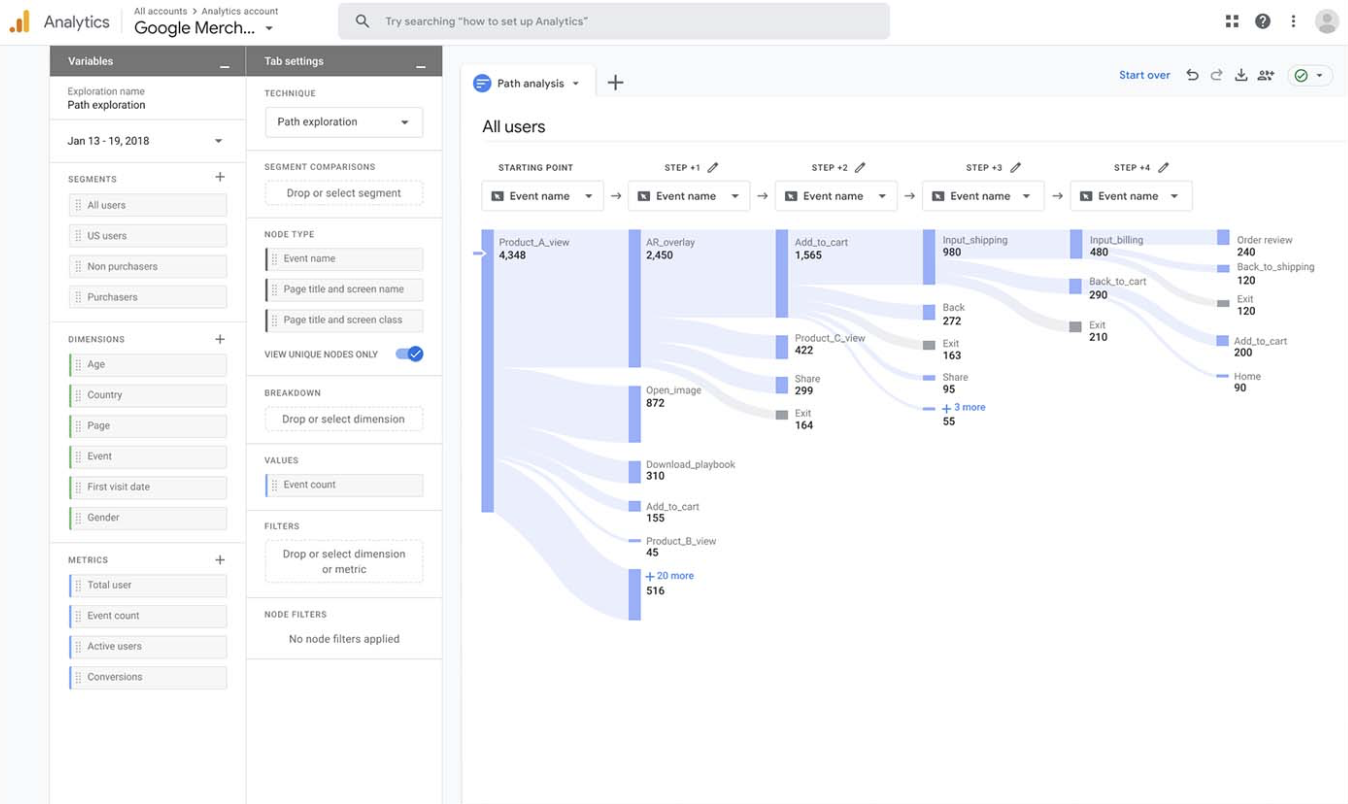
\includegraphics{img/part 2/4-1.png}

}

\caption{그림 18: Google Analytics의 데이터 시각화 화면}

\end{figure}%

\subsection{Power BI}\label{power-bi}

\textbf{Power BI}는 Microsoft에서 제공하는 비즈니스 분석 서비스로,
데이터를 시각화하고 공유 가능한 보고서를 생성하며, 인사이트를 도출하는
클라우드 기반 솔루션입니다. 사용 방법은 Power BI Desktop 설치 후, 다양한
데이터 소스를(Excel, SQL Server 등) 연결하고, 실시간 데이터 가져오기
하여 분석을 시행합니다. Power BI Desktop에서 보고서 작성 후에는 Power BI
서비스(웹)에서 공유 및 대시보드를 관리합니다. 이를 통해 사용자들은
데이터 기반의 의사 결정을 내릴 수 있습니다. (17)

\href{https://powerbi.microsoft.com/ko-kr/guidedtour/power-platform/power-bi/2/1}{Microsoft
Guided Tours}

\subsection{주요 서비스}\label{uxc8fcuxc694-uxc11cuxbe44uxc2a4-1}

\begin{itemize}
\tightlist
\item
  \textbf{데이터 통합}: 다양한 데이터 소스(엑셀, SQL 데이터베이스,
  클라우드 서비스 등)와 연결하여 데이터를 통합합니다. 특히 Microsoft
  제품과의 통합에 강점을 가집니다.
\item
  \textbf{대시보드 생성}: 실시간 데이터 시각화와 대시보드를 생성하여
  데이터를 한눈에 파악할 수 있습니다.
\item
  \textbf{보고서 작성}: 다양한 시각화 도구를 사용하여 상세한 보고서를
  작성하고 분석할 수 있습니다.
\item
  \textbf{모바일 접근성}: 모바일 앱을 통해 언제 어디서나 데이터를
  조회하고 분석할 수 있습니다.
\item
  \textbf{AI 통합}: 인공지능 기능을 통해 예측 분석과 자동화된 인사이트를
  제공합니다
\item
  \textbf{사용자 친화적 인터페이스와 협업 지원}: 직관적이고 사용하기
  쉬운 인터페이스를 제공하고, 팀 내에서 보고서를 공유하고 협업할 수
  있습니다.
\item
  \textbf{단점:} 초보자에게는 초기 설정이 복잡할 수 있습니다. 무료
  버전의 기능이 제한적이며, 대용량 데이터를 처리하는 데 제한이 있을 수
  있습니다.
\end{itemize}

\begin{figure}[H]

{\centering 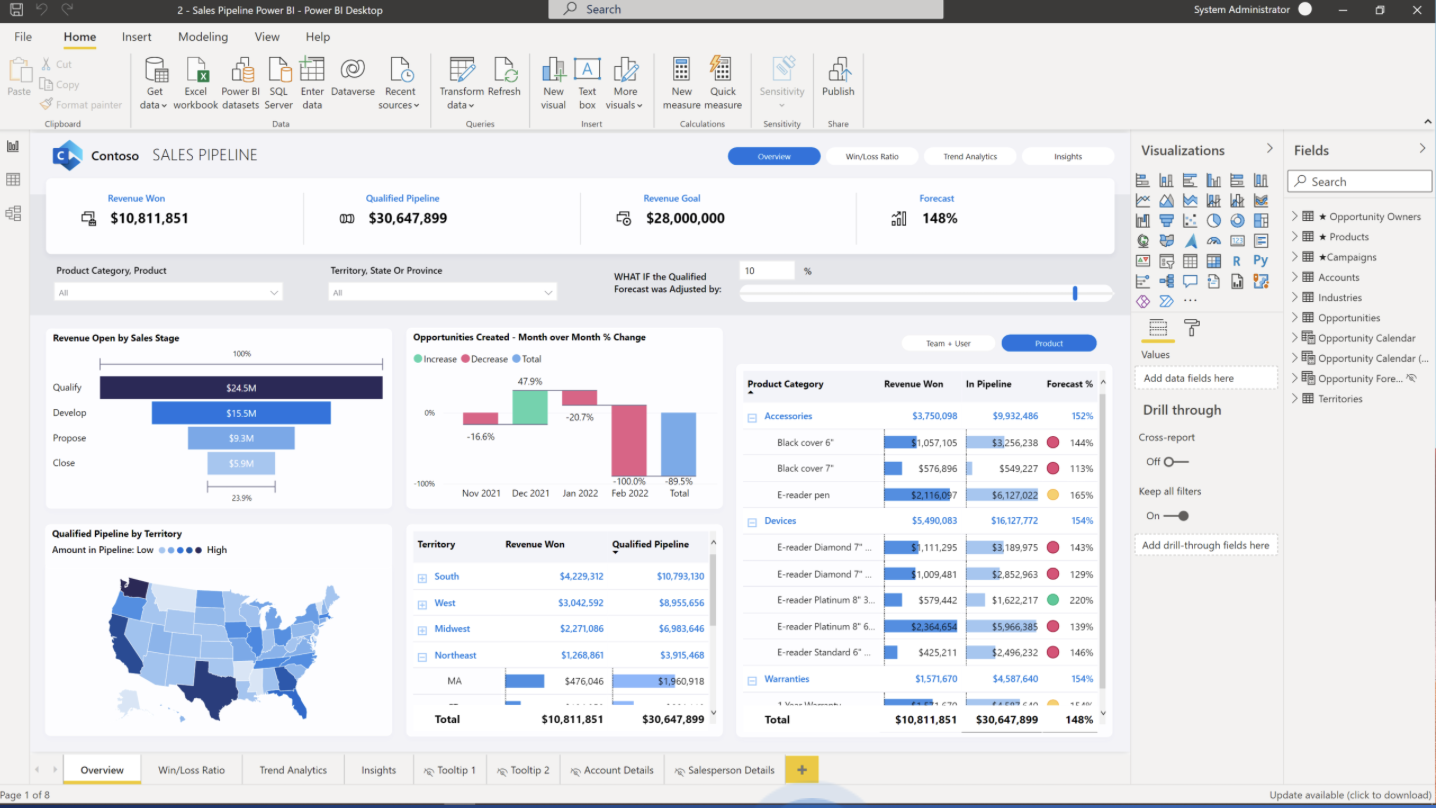
\includegraphics{img/part 2/4-2.png}

}

\caption{그림 19: Power BI의 데시보드 구성 화면}

\end{figure}%

\subsection{Tableau}\label{tableau}

\textbf{Tableau}는 데이터를 시각적으로 분석하고 이해할 수 있게 돕는
비즈니스 인텔리전스(BI) 도구입니다.

Tableau는 고급 데이터 시각화 기능에 강점을 갖고 있어, 히트맵, 트리맵,
버블 차트 등 다양한 고급 시각화 기능을 제공하고, 사용자가 대시보드를
인터렉티브하게 데이터 탐색을 할 수 있으며, 데이터 시각화를 스토리 형태로
구성해 프레젠테이션하고, 지리적 데이터를 시각화하고 분석하는 강력한
기능을 제공합니다. (18)

\href{https://www.tableau.com/ko-kr/products/tableau}{Tableau}

\subsection{주요 서비스}\label{uxc8fcuxc694-uxc11cuxbe44uxc2a4-2}

\begin{itemize}
\tightlist
\item
  \textbf{데이터 통합}: 다양한 소스의 데이터를 통합하여 일관된 분석
  가능합니다.
\item
  \textbf{시각화 도구}: 드래그 앤 드롭 방식으로 손쉽게 고급 시각화
  차트와 대시보드를 생성합니다.
\item
  \textbf{AI 및 ML 통합}: 인공지능과 머신러닝을 통해 예측 분석 및
  인사이트를 제공합니다.
\item
  단점: 고급 기능을 완전히 익히는 데 시간이 필요합니다.
\end{itemize}

\begin{figure}[H]

{\centering 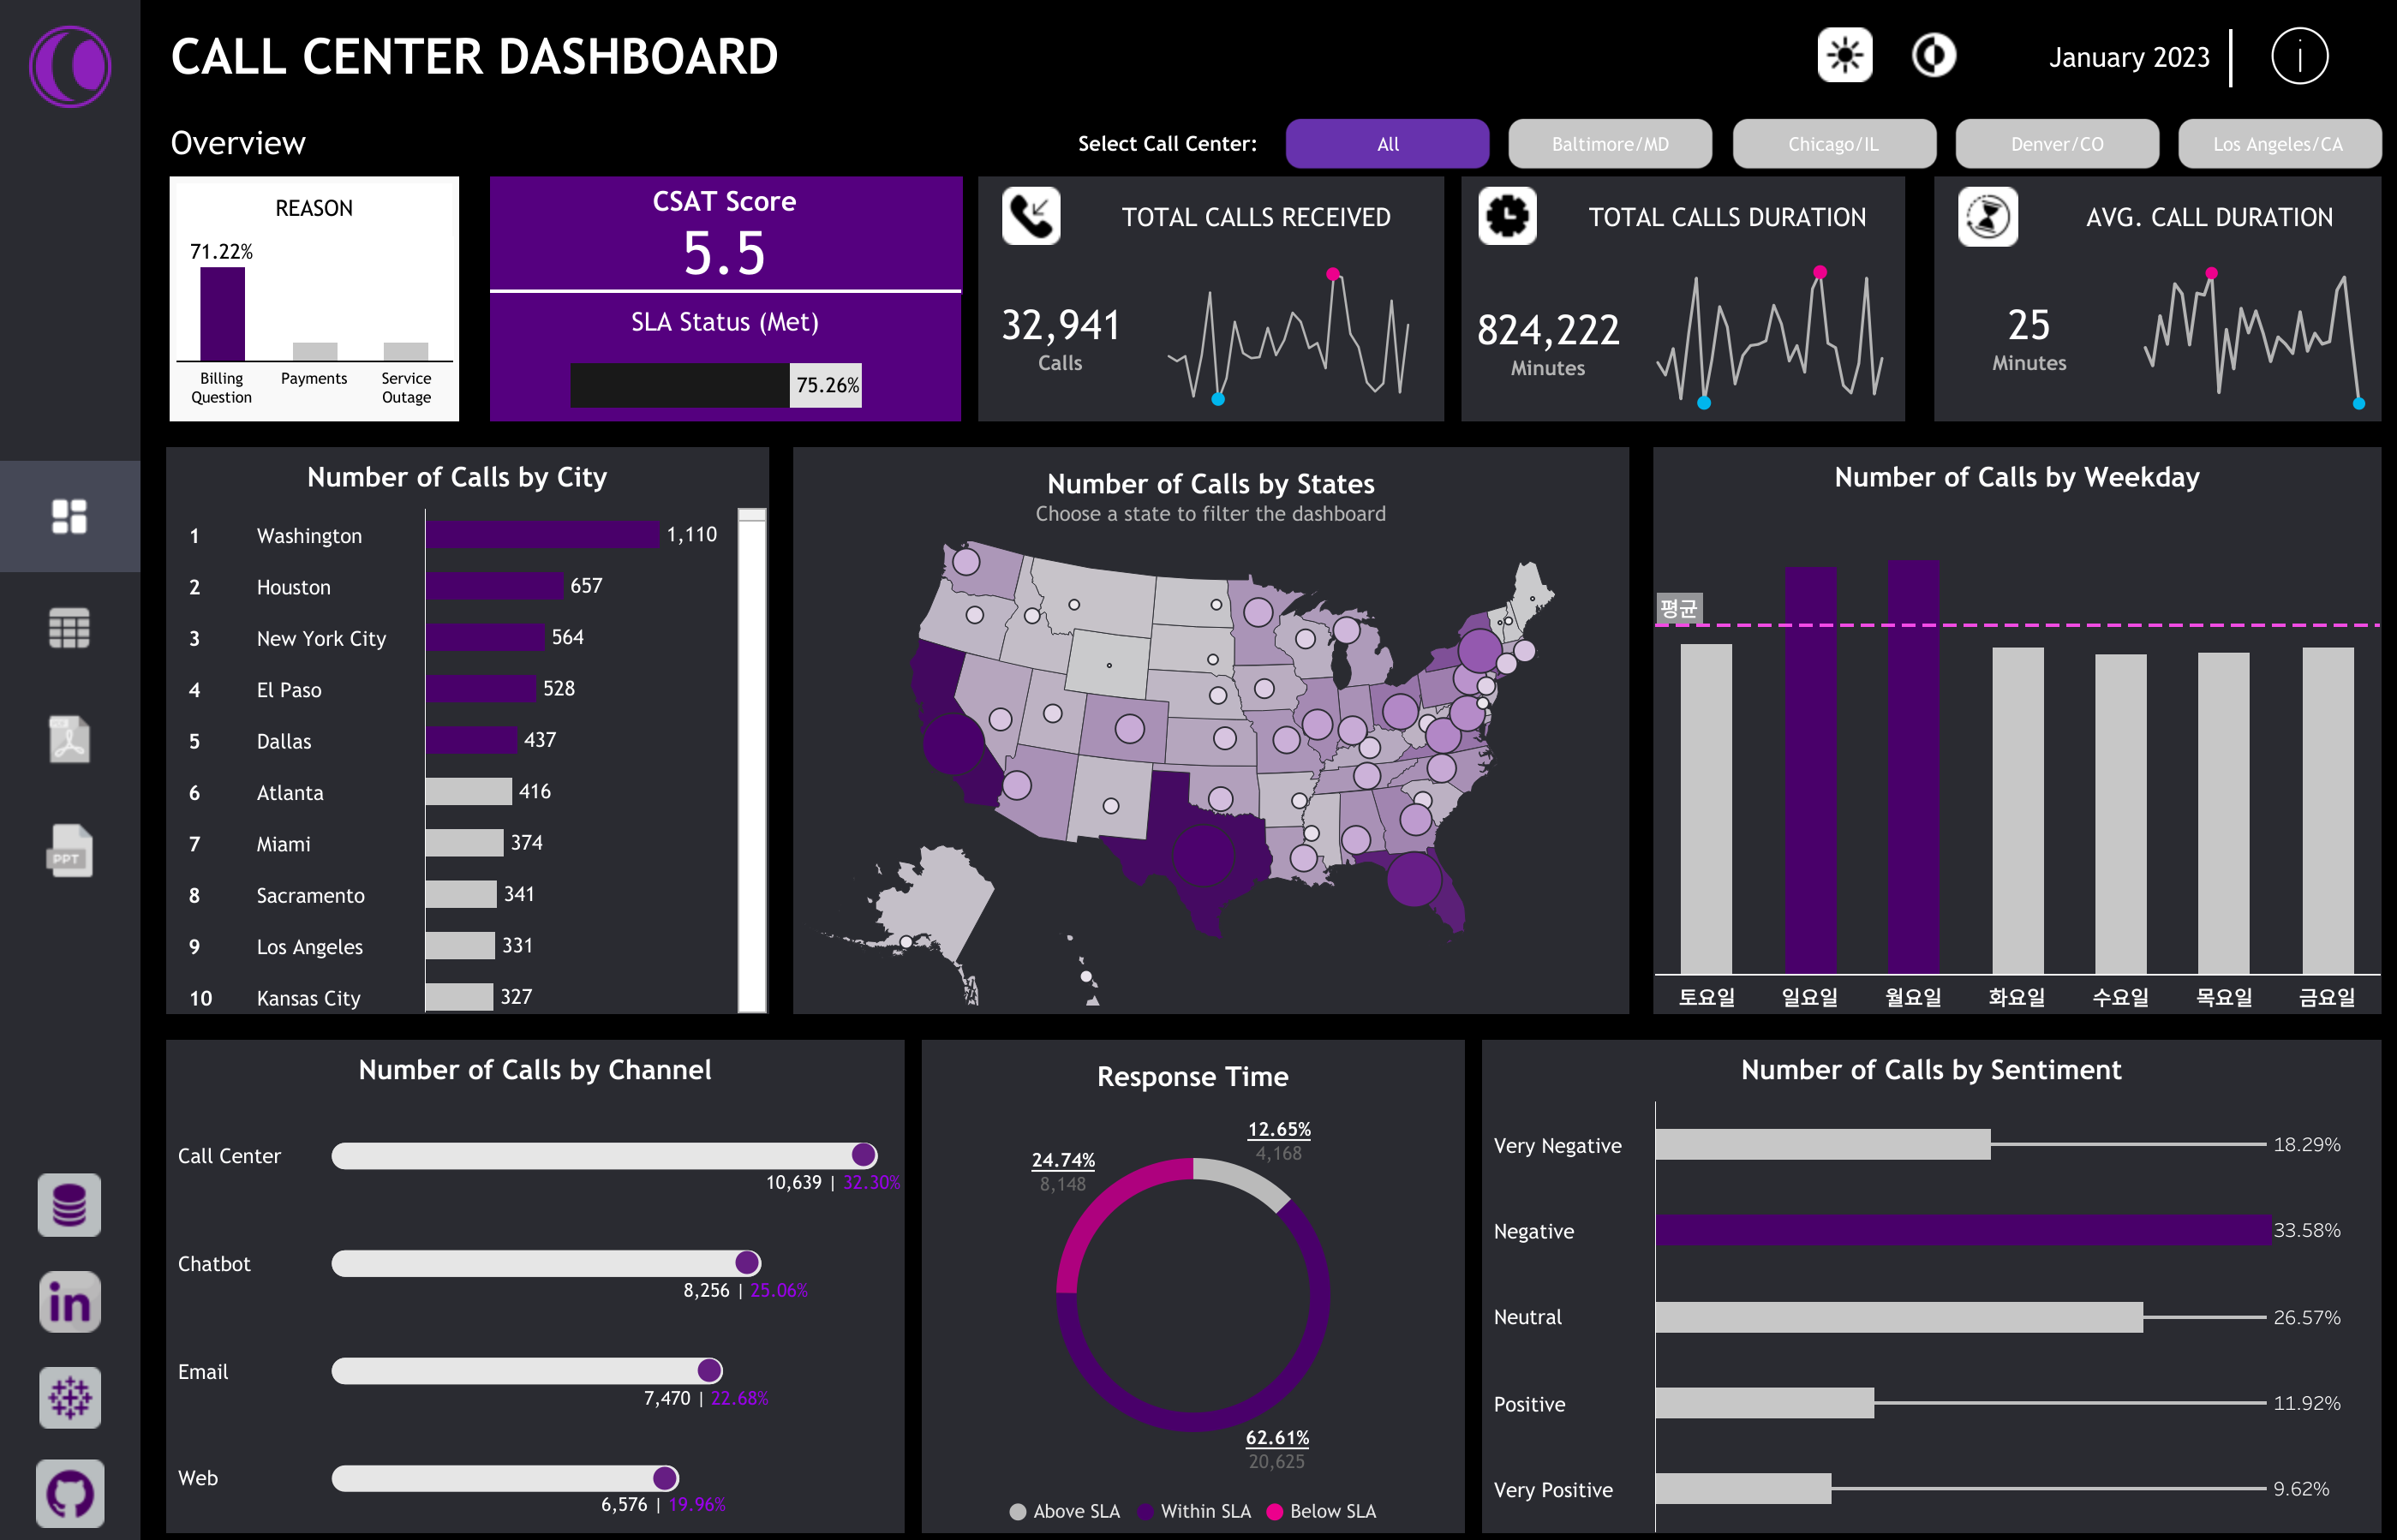
\includegraphics{img/part 2/4-3.png}

}

\caption{그림 20: Tableau를 사용한 인터렉티브 대시보드}

\end{figure}%

이 세가지 서비스는 세계적으로 가장 많이 사용되는 데이터 분석 서비스이고,
최근에는 AI 기술을 사용한 시각화 및 예측 서비스가 강화되는 추세입니다.
Google Analytics는 주로 웹사이트 분석에, Power BI는 비즈니스 인텔리전스
및 데이터 분석에, Tableau는 고급 데이터 시각화에 좀 더 특화되어 있다고
할 수 있습니다.

\subsection{Beusable}\label{beusable}

\textbf{Beusable}은 UX를 위한 데이터 분석에 특화된 국내 서비스로, 사용자
경험을 개선하기 위해 시각화된 데이터 분석 기능을 제공합니다. 주요
기능으로는 Journey Map과 UX Heatmap이 있으며, 이를 통해 고객 여정을
시각적으로 파악하고, 문제 구간을 분석하여 개선안을 도출할 수 있습니다.
설치가 간편하고, 직관적인 UI를 제공합니다. (19)

\href{https://www.beusable.net/ko/}{Beusable}

\subsection{주요 서비스}\label{uxc8fcuxc694-uxc11cuxbe44uxc2a4-3}

\begin{itemize}
\tightlist
\item
  \textbf{Journey Map}: 고객의 전환 과정을 시각화하여 분석합니다.
\item
  \textbf{UX Heatmap}: 페이지 내 사용자 행동을 시각화하여 문제점을
  파악합니다.
\item
  \textbf{간편한 설치}: 한 줄의 코드 설치로 데이터 수집 및 분석이
  가능합니다.
\end{itemize}

\begin{figure}[H]

{\centering 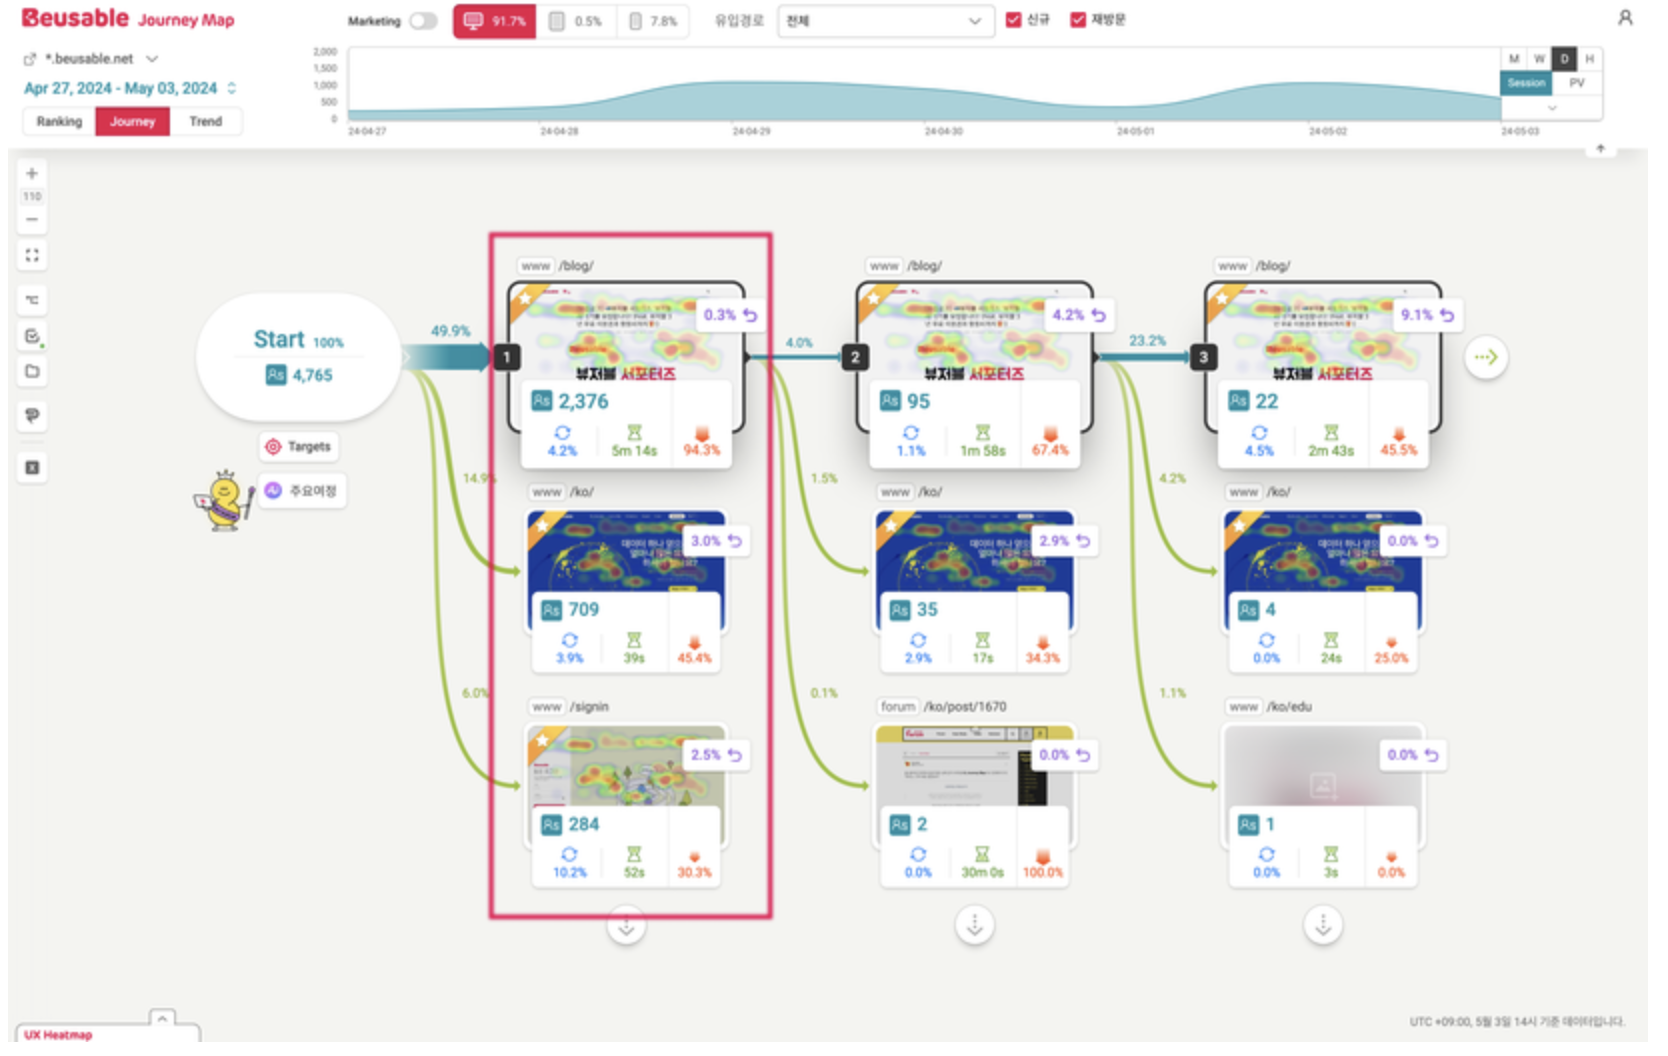
\includegraphics{img/part 2/4-4.png}

}

\caption{그림 21: Beausable의 고객 여정 분석 화면}

\end{figure}%

(문헌 16)Google marketing platform, ``애널리틱스 기능''
\url{https://marketingplatform.google.com/intl/ko/about/analytics/features/}

(문헌 17) Micro Soft, ``Power BI 둘러보기''
\url{https://powerbi.microsoft.com/ko-kr/guidedtour/power-platform/power-bi/2/1}

(문헌 18) Tableau, ``Tableau product''
\url{https://www.tableau.com/ko-kr/products/tableau}

(문헌 19)Beausable, ``Why Beausable'',
\url{https://www.beusable.net/ko/}

\chapter{2-5 Lean UX 프로세스와 데이터 기반
디자인}\label{lean-ux-uxd504uxb85cuxc138uxc2a4uxc640-uxb370uxc774uxd130-uxae30uxbc18-uxb514uxc790uxc778}

\subsection{Lean Design Process의
개념}\label{lean-design-processuxc758-uxac1cuxb150}

목표한 디자인 해결안을 완성하기까지 수행하는 디자인 활동의 내용과 방법,
과정을 정의하는 디자인 프로세스는 디자인의 대상과 사회, 기술적 요구
사항의 변화에 따라 변화하고 있습니다. 현대의 디자인 프로세스는
소프트웨어 기술과의 협업 과정, 비즈니스 방법의 변화에 영향을 받아
애자일(Agile) 디자인 프로세스, 린(Lean)디자인 프로세스라는 특별한 형식의
디자인 프로세스를 적용하는 사례가 많습니다.

`Lean'이라는 단어가 `기대다', `의지하다'라는 의미가 있고 `군살이 없는'
이라는 의미도 있으므로, 린 디자인 프로세스는 편하게 기대어서 하는
디자인, 군살없이 날씬하게 진행하는 디자인 프로세스라는 의미로 생각해볼
수 있습니다. 결국 이 말은 디자인을 하는데, 쓸데 없는 일을 과하게 하지
않고, 시간과 비용의 효율을 추구하는 디자인 방법이라는 뜻입니다. 제품이나
서비스의 생산 주기가 짧고, 소규모 조직으로도 서비스 운영이 가능해진 현대
산업계의 특징을 반영하여 빠른 시간에 적은 인원을 가지고, 꼭 필요한
작업만을 효율적으로 해서 디자인을 수행하는 것이 린 디자인 프로세스의
철학입니다. 이러한 린(Lean) 철학을 UX 디자인 방법론에 가져온 것이 Lean
UX입니다. 그러므로 Lean UX는 UX 디자인의 과정에서 시간과 자원을
효과적으로 사용하여 결과물을 산출하는 방법론이겠죠. UX 디자인 업무가
전통적으로 시간과 조직 역량을 많이 필요로 했던 문제를 해결하고자 한
방법론이라고 하겠습니다. 린 UX는 디자인의 효율화를 추구하는 핵심적인
전략으로 정량 데이터를 적극적으로 활용합니다.

'린 스타트업 실전 UX'라는 책에서 저자(Laura Klein)는 린 UX에 대하여 Lean
비즈니스 환경에 적합한 UX 디자인을 말하는 것으로, 어떤 지표(KPI: Key
Performance Indicator)가 비즈니스를 이끄는지 알아내고, 이러한 지표를
개선하기 위해 해결해야할 고객의 문제가 무엇인지 이해하고(Hypothesis),
고객의 어려움을 개선하는 데 필요한 아이디어를 도출한 다음(MVP: Minimum
Viable Product), 그게 적합한 아이디어인지 검증(A/B testing)하는 것이라고
설명했습니다. (20)

갑자기 낯선 용어들이 많이 나오죠? 괄호 안의 전문 용어들을 빼고 조금 쉽게
서술해 보면 린 UX는 어떤 비즈니스가 잘 되고 있는지를 측정하는 지표 값을
찾고, 이 값을 원하는 목표 값까지 달성하기 위하여 디자인을 수행한 뒤, 그
디자인이 성공했는지를 판단하기 위해 이전 디자인의 지표값과 개선 디자인의
지표값을 비교하여 평가한다는 의미입니다. 내용을 다시 해석해 보면 `지표
값' 이라는 정량 데이터가 있고, 이 데이터를 `목표 값'의 정량 데이터로
변환 시키도록 디자인을 한 뒤, 디자인 개선 후의 `지표 값'이 `목표 값'
수준으로 달성 되었는지를 정량적(통계적)으로 판단한다는 뜻이니,
전체적으로 정량 데이터의 측정과 평가를 중심으로 진행하는 디자인
방법론이네요. 그래서 Lean UX는 결국 데이터에 근거하여 디자인 의사 결정을
수행하는 데이터 기반 디자인 방법론의 하나입니다.

\subsection{Lean UX에 사용하는 주요
용어들}\label{lean-uxuxc5d0-uxc0acuxc6a9uxd558uxb294-uxc8fcuxc694-uxc6a9uxc5b4uxb4e4}

Lean UX를 수행하기 위하여 이해해야하는 KPI, Hypothesis, MVP, A/B
테스팅의 개념을 아래와 같이 정리하였습니다. 각각의 개념은 이후의 실습
프로젝트를 수행하면서 더 명확하게 이해할 수 있을 것입니다.

\begin{itemize}
\item
  KPI(Key Performance Indicator)

  \textbf{KPI}는 조직이나 프로젝트의 목표 달성 정도를 측정하는 데
  사용되는 핵심 성과 지표를 의미합니다. KPI를 통해 프로젝트의 진행
  상황을 모니터링하고, 목표 달성을 위해 필요한 조치를 취할 수 있습니다.
  예를 들어, 새로운 앱의 성공을 측정하기 위한 KPI로 월간 활성 사용자 수,
  사용자 유지율, 평균 세션 시간 등을 KPI로 설정하고, 이 값으로 앱의
  성과를 평가하고 필요한 개선점을 파악할 수 있습니다.

  주요 특징:

  \begin{enumerate}
  \def\labelenumi{\arabic{enumi}.}
  \tightlist
  \item
    \textbf{구체적이고 측정 가능함}: 명확하고 구체적으로 정의되어야
    하며, 수치로 측정 가능해야 합니다.
  \item
    \textbf{목표 지향적}: 조직이나 프로젝트의 목표와 직접적으로 연결되어
    있어야 합니다.
  \item
    \textbf{주기적 평가}: 정기적으로 평가하여 진행 상황을
    모니터링합니다.
  \end{enumerate}
\item
  Hypothesis

  \textbf{가설}은 특정한 질문이나 문제에 대한 예상 답변을 제시하는
  것입니다. 제품이나 기능의 개발 전, 이를 통해 어떤 결과가 나올지를 미리
  예측하고 테스트하는 과정을 의미합니다. Lean UX에서는 가설을 바탕으로
  실험을 진행하고, 그 결과를 통해 제품을 개선합니다. 예를 들어, ``앱의
  새로운 알림 기능을 제공하면 앱을 더 자주 사용할 것이다''라는 가설을
  세우고, 이를 테스트하기 위해 새로운 알림 기능을 출시한 후 사용자
  반응을 분석합니다.

  주요 특징:

  \begin{enumerate}
  \def\labelenumi{\arabic{enumi}.}
  \tightlist
  \item
    \textbf{명확한 진술}: 가설은 구체적이고 명확하게 진술되어야 합니다.
  \item
    \textbf{검증 가능}: 실험을 통해 가설의 진위 여부를 확인할 수 있어야
    합니다.
  \item
    \textbf{피드백 중심}: 사용자 피드백을 통해 가설을 검증하고 개선.
  \end{enumerate}
\item
  MVP(Minimum Viable Product)

  \textbf{MVP}란 제품 개발 과정에서 최소한의 기능만을 갖춘 제품을
  의미합니다. 이 제품은 사용자에게 실질적인 가치를 제공하면서도 개발에
  소요되는 시간과 비용을 최소화하는 것이 목적입니다. MVP를 통해 빠르게
  시장에 제품을 출시하고, 사용자로부터 피드백을 받아 제품을 개선해 나갈
  수 있습니다.

  주요 특징:

  \begin{enumerate}
  \def\labelenumi{\arabic{enumi}.}
  \tightlist
  \item
    \textbf{최소한의 기능}: 제품의 핵심 기능만 포함.
  \item
    \textbf{빠른 출시}: 개발 시간을 줄여 빠르게 시장에 출시.
  \item
    \textbf{사용자 피드백}: 실제 사용자로부터 피드백을 받아 제품을 개선.
  \end{enumerate}
\item
  A/B 테스팅

  A/B 테스트는 디자인의 구현 과정에서 화면이나 기능을 여러 버전으로
  만들어서 서로 다른 사용자 그룹에 각기 다른 것을 보여주고 어떤 버전이
  최선의 지표를 이끌어 내는지 찾아내는 기법입니다. A/B 테스트의 목적은
  통계적으로 의미있는 데이터를 활용해서 사업적 중요성(KPI)을 기준으로
  제품에 관련된 더 나은 의사결정을 하려는 것입니다. 예를 들어,
  웹사이트의 버튼 색상을 A는 파란색, B는 빨간색으로 설정하여 어떤 색상이
  더 많은 클릭을 유도하는지 테스트합니다.

  주요 특징:

  \begin{enumerate}
  \def\labelenumi{\arabic{enumi}.}
  \tightlist
  \item
    \textbf{두 가지 버전}: A 버전과 B 버전, 두 가지 버전으로 나눔.
  \item
    \textbf{실험군과 통제군}: 사용자 그룹을 나눠 각각 다른 버전을
    사용하게 함.
  \item
    \textbf{성과 측정}: 각 버전의 성과를 비교하여 더 나은 쪽을 선택.
  \end{enumerate}
\end{itemize}

\subsection{Lean UX Process Diagram (Learn\textgreater{} Build
\textgreater{} Measure \textgreater{} Learn \textgreater 의
반복)}\label{lean-ux-process-diagram-learn-build-measure-learn-uxc758-uxbc18uxbcf5}

데이터를 중심으로 의사결정을 하는 린 UX의 또 하나의 중요한 특징은
반복적인 수행 과정입니다.

데이터를 통하여 알게된(Learn) 인사이트를 가지고 KPI를 개선하는
아이디어(가설)를 내고, 이것을 MVP로 개발하여(Build) 아이디어가 잘
작동하는지는 검증(Measure)하고, 검증 데이터를 바탕으로(Learn) 다시
개선안을 내고, 이것을 MVP로 개발하여(Build) 아이디어가 잘 작동하는지는
검증(Measure)하는 반복적인 과정을 원하는 수준의 KPI에 도달할 때까지
반복하여 진행합니다. 최종 디자인 목표가 달성될 때까지
Learn\textgreater{} Build \textgreater{} Measure \textgreater{} Learn
\textgreater 의 과정은 반복됩니다. 이 과정을 그림으로 표현하면 {[}그림
22{]}과 같습니다.

애플은 앱 디자인 프로세스를 설명할 때 같은 개념을 Think\textgreater{}
Make\textgreater{} Check\textgreater{} Think의 반복적 프로세스로
설명했습니다.

\begin{figure}[H]

{\centering 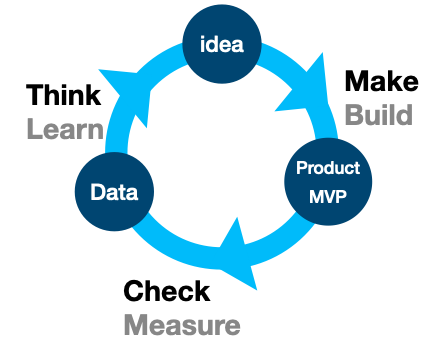
\includegraphics{img/part 2/5-1.png}

}

\caption{그림 22: 순환적이고, 반복적인 Lean UX 디자인 프로세스}

\end{figure}%

\begin{itemize}
\tightlist
\item
  다음은 참고도서의 저자인 Laura Klein이 Lean UX에 대하여 설명하는
  영상입니다.(21)
\end{itemize}

\url{https://www.youtube.com/watch?v=7NkMm5WefBA}

우리는 Lean UX의 디자인 프로세스인 Leran \textgreater{} Build
\textgreater{} Measure \textgreater{} Learn의 단계를 따라서 실습 과제를
수행하게 됩니다. 그럼 다음 장에서는 Lean UX의 과정을 따라서 데이터 기반
디자인 방법을 실습해 볼까요?

(문헌 20) 로라 클라인, (김수영, 박기석 역), 『린 스타트업 실전 UX』,
한빛미디어,(2014)

(문헌 21) Google Developers, ``UXD: What is Lean UX?'',
https://www.youtube.com/watch?v=7NkMm5WefBA

\bookmarksetup{startatroot}

\chapter*{References}\label{references}
\addcontentsline{toc}{chapter}{References}

\markboth{References}{References}


\backmatter
\printbibliography


\printindex


\end{document}
